	\documentclass[12pt,a4paper]{report}
\usepackage{amsmath}
\usepackage{amsfonts}
\usepackage{amssymb}
\usepackage[english]{babel} %type ngerman if you are using a PC of the university
\usepackage{babelbib}
\usepackage[T1]{fontenc}
\usepackage[sc]{mathpazo}
\usepackage[utf8]{inputenc}
\usepackage{graphicx}
\usepackage[width=150mm,top=25mm,bottom=25mm]{geometry}
%\usepackage{units}
\usepackage{fancyhdr}
\pagestyle{fancy}

\renewcommand{\chaptermark}[1]{\markboth{#1}{}}

%Chapter title on even header and section title in odd header
\fancyhf{} % clear the headers
\fancyhead[R]{%
   % We want italics
   \itshape
   % The chapter number only if it's greater than 0
   \ifnum\value{chapter}>0 \chaptername\ \thechapter. \fi
   % The chapter title
   \leftmark}
\fancyfoot[C]{\thepage}

\fancypagestyle{plain}{
  \renewcommand{\headrulewidth}{0pt}
  \fancyhf{}
  \fancyfoot[C]{\thepage}
}

\setlength{\headheight}{14.5pt}
\makeatletter
\setlength{\@fptop}{0pt}
\makeatother
%\usepackage{kantlipsum} % for the mock text
\usepackage{enumerate} % enumerados
\usepackage{float} % here for H placement parameter
\usepackage{colortbl}
\usepackage{xcolor}
\definecolor{mygray}{gray}{0.8}
\usepackage{xfrac}
\usepackage{booktabs} 
\usepackage{colortbl} 
\usepackage{color}   %May be necessary if you want to color links
\usepackage{hyperref}
\usepackage{setspace}
\usepackage{caption}
\usepackage{subcaption}
\usepackage{titlesec}
\usepackage{tikz}
\usepackage{amsmath}
\usetikzlibrary{calc,positioning,shadows.blur,decorations.pathreplacing}
\usepackage{etoolbox}
\usepackage{anyfontsize}
\usepackage[toc,page]{appendix}
%\titleformat{\chapter}{\normalfont\bfseries}{\thechapter}{1em}{\Huge}
\titleformat{\chapter}{\normalfont\bfseries}{\huge\thechapter}{1em}{\Huge}
\usepackage{nicefrac}
\onehalfspacing
\hypersetup{
    colorlinks=false, %set true if you want colored links
    linktoc=all,     %set to all if you want both sections and subsections linked
    linkcolor=blue,  %choose some color if you want links to stand out
	}
\author{Youssef El Mard Bouziani}
\title{Transversalimpulsverteilung geladener Teilchen in Proton-Proton-Kollisionen bei  $\sqrt{s} = 5.02$ TeV in ALICE}
\parindent 0ex



\begin{document}
%NEW COMMANDS
%https://texample.net/media/tikz/examples/PDF/periodic-table-of-chemical-elements.pdf
\newcommand{\Quark}[5]
{
  \begin{minipage}{0.cm}
    %\centering
      %{\scriptsize \text{#1}  \hfill  \footnotesize #2}%
      {\hfill \footnotesize \text{ #3} }
        % {\centering \footnotesize \textbf{#5}\\}
  \end{minipage}
 {\raisebox{40pt}{\makebox[1em][l]{\footnotesize \textbf{#1}}}%
 \hspace{2.3cm} \raisebox{40pt}{\makebox[3em][l]{\footnotesize \textbf{#2} }} \hspace{-3.1cm} 
 \parbox[t][1em]{3em}{\centering{\fontsize{40}{40}\selectfont  #4}	}\hspace*{1em}   %Amb \parbox[t][1em]{2em} es la carga electrica surt del requadre     
    \parbox[c][6em]{0em}{\vspace{1.4cm}\hspace{-2.7cm}\centering \footnotesize \textbf{#5}}   
}
}
  \tikzstyle{QuarkFill} = [fill=blue!15]
  \tikzstyle{LeptonFill} = [fill=red!15]
  \tikzstyle{BosonFill} = [fill=green!15]
  \tikzstyle{quark} = [draw=blue, very thick, rounded corners=2mm, QuarkFill,  minimum height={2.6cm+2pt}, minimum width=2.cm, node distance=2.cm ]
    \tikzstyle{lepton} = [draw=red, very thick, rounded corners=2mm, LeptonFill,  minimum height={2.6cm+2pt}, minimum width=1.5cm, node distance=2.cm ]
    \tikzstyle{boson} = [draw=green, very thick, rounded corners=2mm, BosonFill,  minimum height={2.6cm+2pt}, minimum width=1.5cm, node distance=2.cm ]
   
\newcommand{\pt}{$p_\text{T}$ }
\newcommand{\raa}{$R_\text{AA}$ }
\newcommand{\rled}{$R_\text{PbPb}$ }
\definecolor{headerBlue}{RGB}{104, 104, 255} %blue RICHTIG headerBlue
\definecolor{headerRed}{RGB}{126, 0, 33} %red
\definecolor{bodyBlue}{RGB}{228,232,244} %light blue

\begin{titlepage}
\begin{center}

\vspace*{4cm}  

\huge{\textbf{Nuclear Modification of charged-particles production at $\sqrt{s_\text{NN}} = 5.02$ TeV in ALICE}}\\[2cm]
\vfill
\Large{\textbf{Master thesis}}\\
Institut für Kernphysik Frankfurt\\
\vfill
%presented by\\[1cm]
by \Large{\textbf{Youssef El Mard Bouziani}}\\[1cm]
\vfill
Fachbereich Physik\\
der Goethe-Universität\\
Frankfurt am Main\\
\vspace*{1cm}
April 2021
\end{center}
\end{titlepage}


\vspace*{22cm}
\large{Erstgutachter: Prof. Dr. Henner Büsching}\\
\large{Zweitgutachter: Prof. Dr. Harald Appelshäuser}
\normalsize
\pagenumbering{roman}
\newpage
\tableofcontents
\newpage

\pagenumbering{arabic}
\setcounter{chapter}{-1}
\pagenumbering{arabic} 
\chapter{Abstract}

\chapter{Introduction}
%Show results in the first chapter of the thesis to have a motivation for your thesis
\label{cha:StdModel}
\section{The Structure of Matter}
\label{sec:DasSMT}
Throughout the twentieth century, successive crucial advances in the field of particle physics led to a revolution of the world-view on the structure of matter and the fundamental forces that govern the universe. Following these developments, it became necessary to consolidate the acquired knowledge into a single theory: the Standard Model, which marked by the end of the 1970s the foundation of modern particle physics. This systematization provided from a theoretical point of view subsequently confirmed experimentally a comprehensive description of the nature of elementary particles and the fundamental interactions they mediate: the electromagnetic, the weak and the strong interaction. \\
All matter in the universe is composed of indivisible particles that lack spatial extension and substructure, the so-called elementary particles. The first particles to be proposed as elementary were the atoms. This picture changed in the early 20th century after it was proved that atoms are made up of a nucleus constituted by protons and neutrons, around which electrons orbit. In the subsequent decades, an extensive number of other subatomic particles were discovered, raising the question among physicists of whether all of them were in fact structureless. The Standard Model sorted out this confusion, historically known as particle zoo, describing the existence of a low number of elementary particles subdivided into two types named quarks and leptons that build all known particles, including protons and neutrons. In addition, the Standard Model clarified that the interactions between quarks and leptons occur by means of an exchange of force-carrier particles, also considered elementary. \\
In order to classify the elementary particles, it is required to consider the immutable and distinguishable physical properties each of them possess. In this regard, the most fundamental distinction between the building blocks of matter and the force-carrier particles lies in the intrinsic angular momentum, known generally as spin, all particles carry, whether or not they are elementary. Particles of half-integer spin in units of the Planck's constant $\hbar$ are named fermions and present an antisymmetric wave function, whereas those of integer spin are known as bosons and their wave function describes a symmetric behavior. In this context, quarks and leptons are considered elementary fermions since their spin is equal to $\nicefrac{\pm 1}{2}$, while the force-carriers, which have a spin $1$, are referred to as gauge bosons.\\
The Standard Model states the existence of six quarks and six leptons, summarized in Figure \ref{SM}. Both groups of elementary fermions are arranged according to the mass in three doublets named generations. Each pair of quarks or leptons have a mass one or two orders of magnitude lower than the pair of the next generation. Furthermore, the electrical charge is another feature used to sort elementary fermions. The triplets composed of elementary fermions from different generations have the same electrical charge, namely $\nicefrac{+2}{3}$ and $\nicefrac{-1}{3}$ for the case of the quarks and $0$ and $-1$ for the one of the leptons. The Standard Model predicts also the occurrence in Nature of antiquarks and antileptons, elementary fermions with identical mass as their counterparts but opposite electrical charge and spin.  \\
The six species or flavours of quarks known at the present day are up $u$, down $d$, charm $c$, strange $s$), top $t$ and bottom $b$. At this point, it should be emphasized that quarks could not yet be observed existing on their own, but only building bound states named hadrons. These composite particles, detected for the first time during the era of the particle zoo, come in two types: hadrons built from three different quarks are called baryons, while those constituted of a quark-antiquark pair mesons. For instance, the quark composition of protons and neutrons, respectively \textit{uud} and \textit{udd}, 
allows to identify them as baryons. All known hadrons, excluding the proton, decay after a given period of time. It should be also noted that since the spin is an additive property, baryons are considered fermionic particles and mesons, by contrast, bosonic particles. \\
The quark composition of a hadron determines intrinsic facets of the particle, which are associated with additive quantities named quark quantum numbers: the well-known electrical charge, a parametrization of the number of quarks called baryon number \textit{B} and other parametrization of the second- and third-generation flavours. However, the valence quarks, i.e. the quarks that determine the identity of a hadron, aren't the only components. In fact, a hadron should be understood as a more complex and dynamic structure that contains, aside from the valence quarks, an amalgam of quark-antiquark pairs named sea quarks in a constant process of creation and annihilation as well as a large number of gluons, the force-carrier of the strong interaction, which will be discussed later. This picture is consistent with the fact that the sum of the masses of the valence quarks of a given hadron doesn't coincide with the observed mass of the hadron, being this significantly larger.  \\
\begin{figure}
\begin{center}
\begin{tikzpicture}[font=\sffamily, x=1.5cm, y=2cm, scale = 0.35, every node/.style={scale=0.6}]
\centering 
\node[name=u, quark] {\Quark{3 MeV}{$\nicefrac{1}{2}$}{$\nicefrac{+2}{3}$}{$\boldsymbol u$}{up}};
 \node [name=c, right=0.1cm of u, quark] {\Quark{1.24 MeV}{$\nicefrac{1}{2}$}{$\nicefrac{+2}{3}$}{$\boldsymbol c$}{charm}};
  \node [name=t, right=0.1cm of c, quark] {\Quark{172.5 GeV}{$\nicefrac{1}{2}$}{$\nicefrac{+2}{3}$}{$\boldsymbol t$}{top}};
  \node [name=d, below=0.1cm of u, quark] {\Quark{6\text{ MeV}}{$\nicefrac{1}{2}$}{$\nicefrac{-1}{3}$}{$\boldsymbol d$}{down}};
  \node [name=s, below=0.1cm of c, quark] {\Quark{95\text{ MeV}}{$\nicefrac{1}{2}$}{$\nicefrac{-1}{3}$}{$\boldsymbol s$}{strange}};
   \node [name=b, below=0.1cm of t, quark] {\Quark{4.2\text{ GeV}}{$\nicefrac{1}{2}$}{$\nicefrac{-1}{3}$}{$\boldsymbol b$}{bottom}};
   
  \node [name=elneu,  below=0.2cm of d, lepton] {\Quark{<\text{2.2}\text{ eV}}{$\nicefrac{1}{2}$}{$0$}{$\boldsymbol  \nu_e$}{electron neutrino}};
  \node [name=elmuon, right=0.1cm of elneu, lepton] {\Quark{<\text{0.17}\text{ MeV}}{$\nicefrac{1}{2}$}{$0$}{$\boldsymbol  \nu_\mu$}{muon neutrino}};
    \node [name=eltau, right=0.1cm of elmuon, lepton] {\Quark{<\text{15.5}\text{ eV}}{$\nicefrac{1}{2}$}{$0$}{$\boldsymbol  \nu_\tau$}{tau neutrino}};
    
      \node [name=ele,  below=0.1cm of elneu, lepton] {\Quark{0.511\text{ MeV}}{$\nicefrac{1}{2}$}{$-1$}{$\boldsymbol e$}{electron}};
  \node [name=muon, right=0.1cm of ele, lepton] {\Quark{105.7\text{ MeV}}{$\nicefrac{1}{2}$}{$-1$}{$\boldsymbol \mu$}{muon}};
    \node [name=tau, right=0.1cm of muon, lepton] {\Quark{1.777\text{ GeV}}{$\nicefrac{1}{2}$}{$-1$}{$\boldsymbol\tau$}{tau}};
   
 \node [name=gluon,  right=0.2cm of t, boson] {\Quark{$0$}{$1$}{$0$}{$\boldsymbol  g$}{gluon}};
 \node [name=photon,  right=0.2cm of b, boson] {\Quark{$0$}{$1$}{$0$}{$\boldsymbol  \gamma$}{photon}};
 \node [name=gluon,  right=0.2cm of eltau, boson] {\Quark{91.19 GeV}{$1$}{$0$}{$\boldsymbol  Z$}{\textit{Z} boson}};
 \node [name=gluon,  right=0.2cm of tau, boson] {\Quark{80.39 GeV}{$1$}{$\pm$1}{$\boldsymbol  W$}{\textit{W} boson}};
\end{tikzpicture}
 \caption{(Das Bild ist nicht fertig!) Elementary particles of the Standard Model.}
 \label{SM}
\end{center}
\end{figure}
\hspace{-0.53cm} As already mentioned, six flavours of leptons are known at this time: three electrically charged leptons, the electron $e$, the muon $\mu$ and the tau $\tau$, and the corresponding electrically neutral leptons that complete each generation, the electron neutrino $\upsilon_{e}$, the muon neutrino $\upsilon_{\mu}$ and the tau neutrino $\upsilon_{\tau}$. In contrast to quarks, leptons don't arrange themselves to form composite particles, with the big exception of the electron shell of an atom, and can exist on their own. \\
According to our actual understanding, all observed phenomenon at subatomic level, such as the formation of composite particles or the particle decays, manifest themselves by means of the existence of three fundamental interactions: the electromagnetic, the weak and the strong interaction. In modern particle physics, each of these interactions is explained as an exchange of quanta of elementary bosons between the elementary particles that exert the force. In order to experience a given fundamental force, an elementary particle must carry the corresponding charge. Particles are charged in different magnitudes, which determines the intensity with they create or undergo the force. \\
The force-carrier particle of the electromagnetic interaction is named photon $\gamma$, a massless boson that mediates the attraction and repulsion forces between all electrically charged particles. In the case of the weak interaction, which all elementary fermions can experience, there are three massive mediators: one electrically neutral, namely the $Z$ boson, and two electrically charged, the $W^{\pm}$ bosons. Finally, the strong interaction is mediated by the already introduced gluon $g$. The charge of the strong interaction is called color, but it should not be mistaken for the concept generally known and described by the optical physics. Quarks are the only elementary fermions that have color charge and therefore gluons can couple to them. In addition to quarks, gluons carry also color what allows them to couple to themselves, a particularity only present in the strong interaction. The basic processes of the strong interaction are described by a theory named quantum chromodynamics (QCD). Since some of these processes represent a key knowledge for the understanding of this thesis, this theory will be treated in the coming section more exhaustive.

\section{Quantum Chromodynamics}
\section{Phase diagram and Quark-Gluon-Plasma}
\section{Physics of particle collisions (pp, A-A col.)}
%https://arxiv.org/pdf/1110.5530.pdf
\section{(charged particle) \pt spectra and nuclear modification factor}
In order to understand $R_{AA}$ 
explain pseudorapidity
\section{Monte Carlo simulations}
Comparison of spectra with HIJING models

\chapter{The ALICE Experiment at CERN}
%https://arxiv.org/pdf/1402.4476.pdf Performance of the ALICE Experiment at the CERN LHC

\section{The LHC}
\section{ALICE}
\subsection{ITS}
\subsection{TPC}
%https://www.uni-frankfurt.de/46491136/Generic_46491136.pdf
explain clusters
\subsection{Track reconstruction}
Explain track variables  %https://cds.cern.ch/record/2045797/files/Report.pdf
\subsection{V0 detectors}
\subsubsection{Centrality determination}

\chapter{Analysis}
Since its theoretical proposal forty years ago, the quark-gluon plasma has been a subject of huge interest in the field of high-energy physics, given that it could offer answers to fundamental questions about the structure of matter. The ALICE experiment at the LHC is dedicated to the study of this exotic state of matter that is believed to form in ultra-relativistic particle collisions. \\
As discussed in the first chapter of this work, the physics of strongly interacting matter can be investigated by means of the nuclear modification factor $R_\text{AA}$ which compares the yield of inclusive charged particles in AA collisions and a corresponding reference measurement in pp collisions. In this chapter, an analysis of transverse momentum distributions in Pb-Pb and in pp collisions at a center-of-mass energy $\sqrt{s_\text{NN}}= 5.02$ TeV measured with ALICE is presented. First, the selected data samples are detailed. Then, the procedures to correct for detector effects that have an impact on the \pt distributions are described. With these corrected \pt distributions the nuclear modification factors are calculated and the results discussed and compared to previous ALICE measurements (cite paper here).
\section{Data sample}
\begin{table}[tb!]
\centering
\renewcommand{\arraystretch}{1.5}
\begin{tabular}{c|c|c|c}
\toprule
\rowcolor{headerBlue} \textbf{System} & \textbf{statistics}  \textbf{(M)} & \textbf{MC generator} &  \textbf{MC statistics } \\
\midrule
             & 560 (FAST) & & \\
\textbf{pp}	 &	 &   PYTHIA + GEANT3  & 25\%  	 \\
 &  318 (CENT)   &  	\\
\hline
\textbf{Pb-Pb} & 110 &  HIJING + GEANT3  & 2\% \\
				 &	   & 		 \\
\bottomrule
%pp FAST und PbPb values token from: https://twiki.cern.ch/twiki/bin/view/ALICE/AliDPGReconstructedDataTakingPeriodsSummary
%pp CENT token from Run Condition Table https://alimonitor.cern.ch/configuration/index.jsp?partition=LHC17p&pass=1&raw_run=&filling_scheme=&filling_config=&fillno=&energy=&intensity_per_bunch=&mu=&interacting_bunches=&noninteracting_bunches_beam_1=&noninteracting_bunches_beam_2=&interaction_trigger=&rate=&beam_empty_trigger=&empty_empty_trigger=&muon_trigger=&high_multiplicity_trigger=&emcal_trigger=&calibration_trigger=&quality=&muon_quality=&physics_selection_status=&comment=&field=&det_aco=&det_ad0=&det_emc=&det_fmd=&det_hlt=&det_hmp=&det_mch=&det_mtr=&det_phs=&det_pmd=&det_spd=&det_sdd=&det_ssd=&det_tof=&det_tpc=&det_trd=&det_t00=&det_v00=&det_zdc=&hlt_mode=&changedon=
\end{tabular}
\caption{Overview of the used data periods, the approximate number of events contained in them and the MC productions they are associated with including the percentage of simulated statistics.}
\label{tab:Periods}
\end{table} 
This thesis will make use of pp and Pb-Pb collisions at $\sqrt{s_\text{NN}}= 5.02$ TeV recorded by ALICE in the years 2017 and 2018 respectively. For the pp data takings, the interaction rate was 50 kHz, while in Pb-Pb it was 7.5 kHz. Furthermore, for each data period there is at least one MC production anchored to it, which simulates the exact same conditions and technical specifications of the detector at the time of data taking. The particle collisions for the MC productions were generated by PYTHIA (cite here) in the case of pp collisions and by HIJING (cite here) for the Pb-Pb collisions, while the corresponding detector response was simulated by GEANT3 (cite here). The limited computing time available for these simulations allows to cover only a percentage of the total statistics present in data. An overview of the number of events contained in each data set is summarized in Table \ref{tab:Periods}. The number of events was measured after the event selection depicted in the following section of this chapter.\\
The examined pp data taking contains two separated data subsets that differ according to the readout configuration: the first data subset corresponds to collisions measured excluding the detector signal of the SDD layers, which in this thesis will be referred to as \textit{FAST} in accordance with ALICE convention. This happens whenever the SDD is inoperable due to its dead time. In contrast, the collisions in the second data subset were reconstructed including the information of the SDD layers. These collisions are labeled as \textit{CENT}. Furthermore, the events of the \textit{CENT} subset were reconstructed also without the SDD information allowing to study the impact of the absence of the SDD layers during the tracking. To this purpose, any observable extracted from \textit{CENT} with SDD and from \textit{CENT} without SDD data can be compared. \\
As shown in Table \ref{tab:Periods}, the \textit{FAST} subset contains almost three times as many events as \textit{CENT}. In this work, these two data takings are combined in order to dispose of all measured pp collisions.  In the big picture, this increase of the statistics should lead to an improvement of the precision of the charged-particle \pt spectra in pp collisions, specially in the high \pt region, which in turn could also enhance the precision of the \raa measurements. 
%https://arxiv.org/pdf/1402.4476.pdf Performance of the ALICE Experiment at the CERN LHC
\section{Trigger and event selection}
\subsection{Trigger}
During the data taking, a trigger decides in real time whether a collision candidate is worth to be stored or not. The ALICE experiment focuses its research activities on the investigation of strongly interacting matter and therefore inelastic collisions are of particular interest. The trigger decision is also motivated by the large detector readout time and a limited data storage capacity which represent obstacles that prevent the recording of all events that take place. Moreover, the trigger is also designed to reject undesired interactions with the beam-gas. \\
The trigger configuration which imposes the smallest bias and thus accepts the majority of the overall inelastic cross section is called minimum bias (MB) trigger. For the data sets used in this thesis, a MB trigger that requires signals both in the V0A and V0C detectors in coincidence with the bunch crossing (MB$_\text{and}$) (cite "Performance of ALICE", s. 22).
\subsection{Selection of events}
\begin{figure}[tb!]
\centering
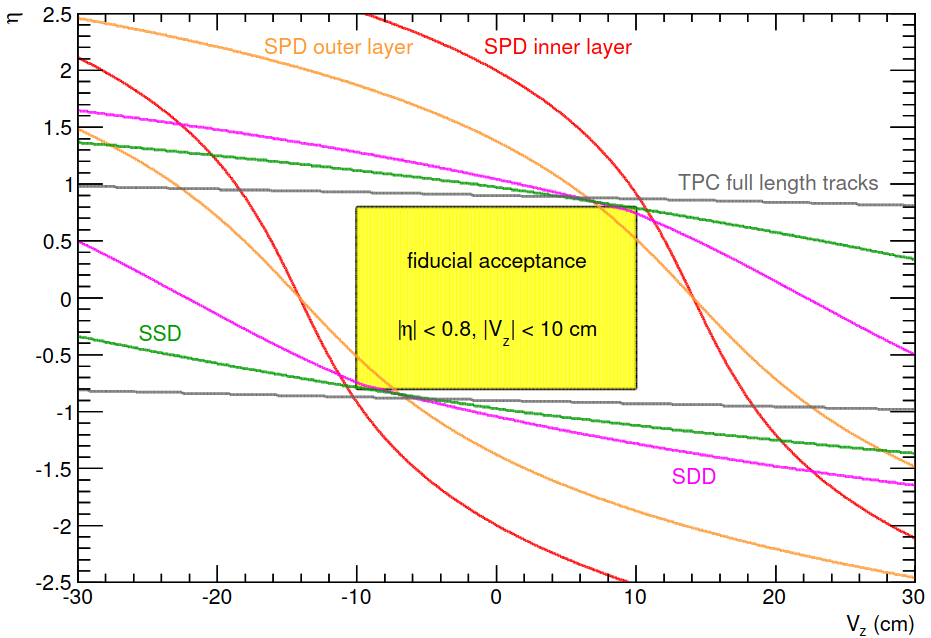
\includegraphics[width=12cm]{Plots/fiducialAcc.png}  
\caption{Pseudorapidity acceptance of the SPD, the SDD, the SSD and the TPC shown as function of the position of the primary vertex along the $z$-axis. The fiducial acceptance represents the region where most tracks can be reconstructed (cite mknichel).}
\label{fiducialAcc}
\end{figure}
In an offline stage of the event selection, collision candidates that satisfy the trigger condition undergo a selection process in order to reduce the contamination with poor quality events. A part of this contamination corresponds to background events, which are caused by the interaction between the LHC beams and the detector material. The beam background is discriminated mainly by means of the signal arrival time of the events in the V0 modules. The arrival time of background events is shorter than the one of a collision produced in the nominal interaction point. This difference is exploited to exclude background events from the data sample. Another source of contamination are the so-called pile-up events, which are multiple collisions occurring within the same bunch crossing. In addition, events produced in a bunch crossing different from the one that triggered the data recording are also considered pile-up. An event is identified as pile-up and removed from the data sample when multiple primary vertices are reconstructed using the information from the SPD in a single triggered event.\\
The pseudorapidity acceptance of the ALICE tracking detectors depends on the position of the primary vertex $\text{V}_z$ along the beam axis $z$ as illustrated in Figure \ref{fiducialAcc} for the ITS subdetectors and the TPC. To ensure a symmetric pseudorapidity  coverage of $|\eta| < 0.8$, the vertex position was restricted to $|V_z| < 10$ cm.$|V_z| < 10$ 
%https://arxiv.org/pdf/1402.4476.pdf
%https://arxiv.org/pdf/1110.5530.pdf
%https://indico.cern.ch/event/752367/contributions/3116617/attachments/1704565/2858687/DPG_AnalysisTutorial_20181129.pdf
\section{Track selection}
\label{TrackSelection}
\begin{table}[tb!]
\renewcommand{\arraystretch}{1.5}
%\rowcolor{bodyBlue}
\centering
\begin{tabular}{l c}
\toprule
\rowcolor{headerBlue}  \textbf{Track variable} &  \textbf{Track cut} \\
\midrule
\multicolumn{2}{c}{\textbf{Selection of primaries}} \\
\midrule
$\text{DCA}_{z}$ & $\leq 2 $ cm\\
$\text{DCA}_{xy}$ & $\leq 7\sigma$ \\
\midrule
\multicolumn{2}{c}{\textbf{ITS selection}} \\
\midrule
at least one hit in the SPD & required \\
ITS refit &  required\\
$\chi^2$ per ITS cluster  & $< 36$ \\
\midrule
\multicolumn{2}{c}{\textbf{TPC selection}} \\
\midrule
TPC refit &  required\\
$\chi^2$ per TPC cluster (pp collisions) & $< 4$ \\
$\chi^2$ per TPC cluster (Pb-Pb collisions) & $< 2.5$ \\
fraction of shared  TPC clusters&  $<  0.4$\\
ratio of crossed rows over findable clusters  & $> 0.8$ \\
geometric length (dead TPC area) & $3$ cm  \\
geometric length (track length) & $130$ cm \\
\midrule
\multicolumn{2}{c}{\textbf{TPC-ITS selection}} \\
\midrule
$\chi^2$ TPC constrained track vs. global track  & $\leq 36$ \\
\bottomrule
\end{tabular}
\caption{Standard track selection criteria used for analysis of primary charged particles in ALICE.}
\label{tab:Cuts}
\end{table}
Primary charged particles traverse the TPC-ITS detector system and follows a trajectory or track that can be reconstructed by means of the procedure described in (cite section). These tracks must fulfil several requirements which aim to select good resolution tracks and reduce the contamination from secondary particles present in the data sample. To this purpose, track selection criteria or track cuts are used in the analysis. They correspond to parameters of track variables related to the quality of the tracks. In addition, the cuts on the $\text{DCA}$ are implemented to eliminate the contamination by secondary particles.\\
Over the years, several analyses on the charged-particle production in ALICE, such as (cite theses), have refined the variations and, as result, the standard track selection listed in Table \ref{tab:Cuts} was established. The track cuts are implemented in both collision systems pp and Pb-Pb for tracks measured in the kinematic range $p_\text{T} > 0.15\text{ GeV}/c$ and $|\eta| < 0.8$, in data and in the corresponding MC productions. 
\iffalse
\subsection{Selection of primaries}
\label{sec:SelOfPrim}
The distance-of-closest approach (DCA) of a track to the primary vertex, introduced in section (cite section), becomes a valuable variable in the supression of secondary particles, which by definition tend to have much larger values than primary particles. For this reason, secondary particles can be removed by setting boundaries to the DCA. In this regard, the standard track selection limits the DCA in beam direction to $2$ cm.\\
With a more aggressive cut, the DCA is also restricted in radial direction by requiring seven standard deviations of the impact parameter resolution, which represents the uncertainty on the DCA to the beam line: %https://indico.cern.ch/event/96989/contributions/2124495/attachments/1114189/1589705/WellsTracking.pdf https://s3.cern.ch/inspire-prod-files-6/6d5c8f5045f30cb63ff7d99fe1a0c79f
\begin{align}
\begin{split}
\text{DCA}_{xy} &\leq 7 \cdot \left(26 + \dfrac{50}{(p_{T}[\text{GeV}/c])^{1.01}}\right) \mu \text{m} \\
& = 7\cdot \sigma
\end{split}
\end{align}
Here, it can be observed that the DCA$_{\text{xy}}$ cut gets more limited the larger the transverse momentum. 
\subsection{ITS selection}
Both mentioned DCA cuts and therefore the selection of primaries are accomplished by virtue of the good DCA resolution achieved by imposing that particles must hit at least one time in the SPD, the innermost layers of the ITS, in order to be selected. Additionally, the ITS refit criterion provides that at least one hit more takes place in one of the ITS layers. \\
A part from that, the ITS track selection has to take also into account the statistical deviation between the reconstructed global track and the fit resulting from reference points from the ITS. This deviation points out that some clusters are assigned to the track incorrectly, which causes a  deterioration of the \pt resolution at high $p_\text{T}$. To prevent that, a statistical variable that evaluates the extent of the deviation named, chi-square, will be limited to $\chi^2$/cluster $< 36$.
\subsection{TPC selection}
Track requirements regarding a refit and a $\chi^2$/cluster cut are also applied in the TPC selection. The TPC refit is implemented using the track reconstruction algorithm twice: from the inside out and in reverse. Further, the $\chi^2$ per TPC cluster is required to stay below a threshold of $4$. \\
The TPC selection focuses also on the detection of fake tracks and tracks that are unintentionally reconstructed multiple times by studying the number of clusters shared by apparently more than one track. These contaminated tracks are excluded adjusting a maximum value for the ratio of shared clusters to all clusters to $0.4$.\\
As already discussed, the clusterization allows the track reconstruction. Since some rows are unable to detect a track due to detector efficiency effects, the number of crossed rows differs frequently from the number of clusters. To correct that, the number of crossed rows includes also those pad rows whose adjacent sides do detect it. Moreover, pad rows that are classified as possible clusters on the basis of the geometry of the track are called findable clusters, a variable more comprehensive than the number of clusters. In this analysis, the ratio of crossed rows over findable clusters must exceed a value of $0.8$. \\
The TPC selection makes a requirement also in relation to the geometric length of the track $L(p_\text{T})$ which is given expressed in cm by:
\begin{equation}
L(p_\text{T}) \geq A - p_\text{T}^{-b}
\end{equation}
where $A=130 \text{ cm}$ corresponds to the minimum length in the active volume of the TPC, $p_\text{T}$ the transverse momentum of the track given in units of $\text{GeV}/c$ and $b=-1.5$ the slope dependency. This calculation excludes the pads situated approximately $3\text{ cm}$ from the sector edges. Furthermore, the geometric track length provides the requirements for the minimum number of crossed rows and of clusters, respectively $0.85\cdot L(p_\text{T})$ rows and $0.7\cdot L(p_\text{T})$ clusters.
\subsection{TPC-ITS selection}
It has been observed that ITS clusters are assigned on occasions improperly to tracks. In further, some tracks can scatter with detector material between the ITS and the TPC. These two effects can result in distortions of the yield	at high $p_\text{T}$. This is prevented through a statistical evaluation between the global track and the constrained track resulting from the TPC information and the primary vertex. The inclusion of the primary vertex can also contribute to a mitigation of the contamination by secondary particles. The statistical evaluation is conducted by means of the $\chi^2_\text{TPC-ITS}$ obtained from the track parameters and their respective uncertainties. Thereby, tracks that exhibit $\chi^2_\text{TPC-ITS}>36$ are rejected.
\fi
\section{Corrections}
\begin{figure}[tb!]
\centering
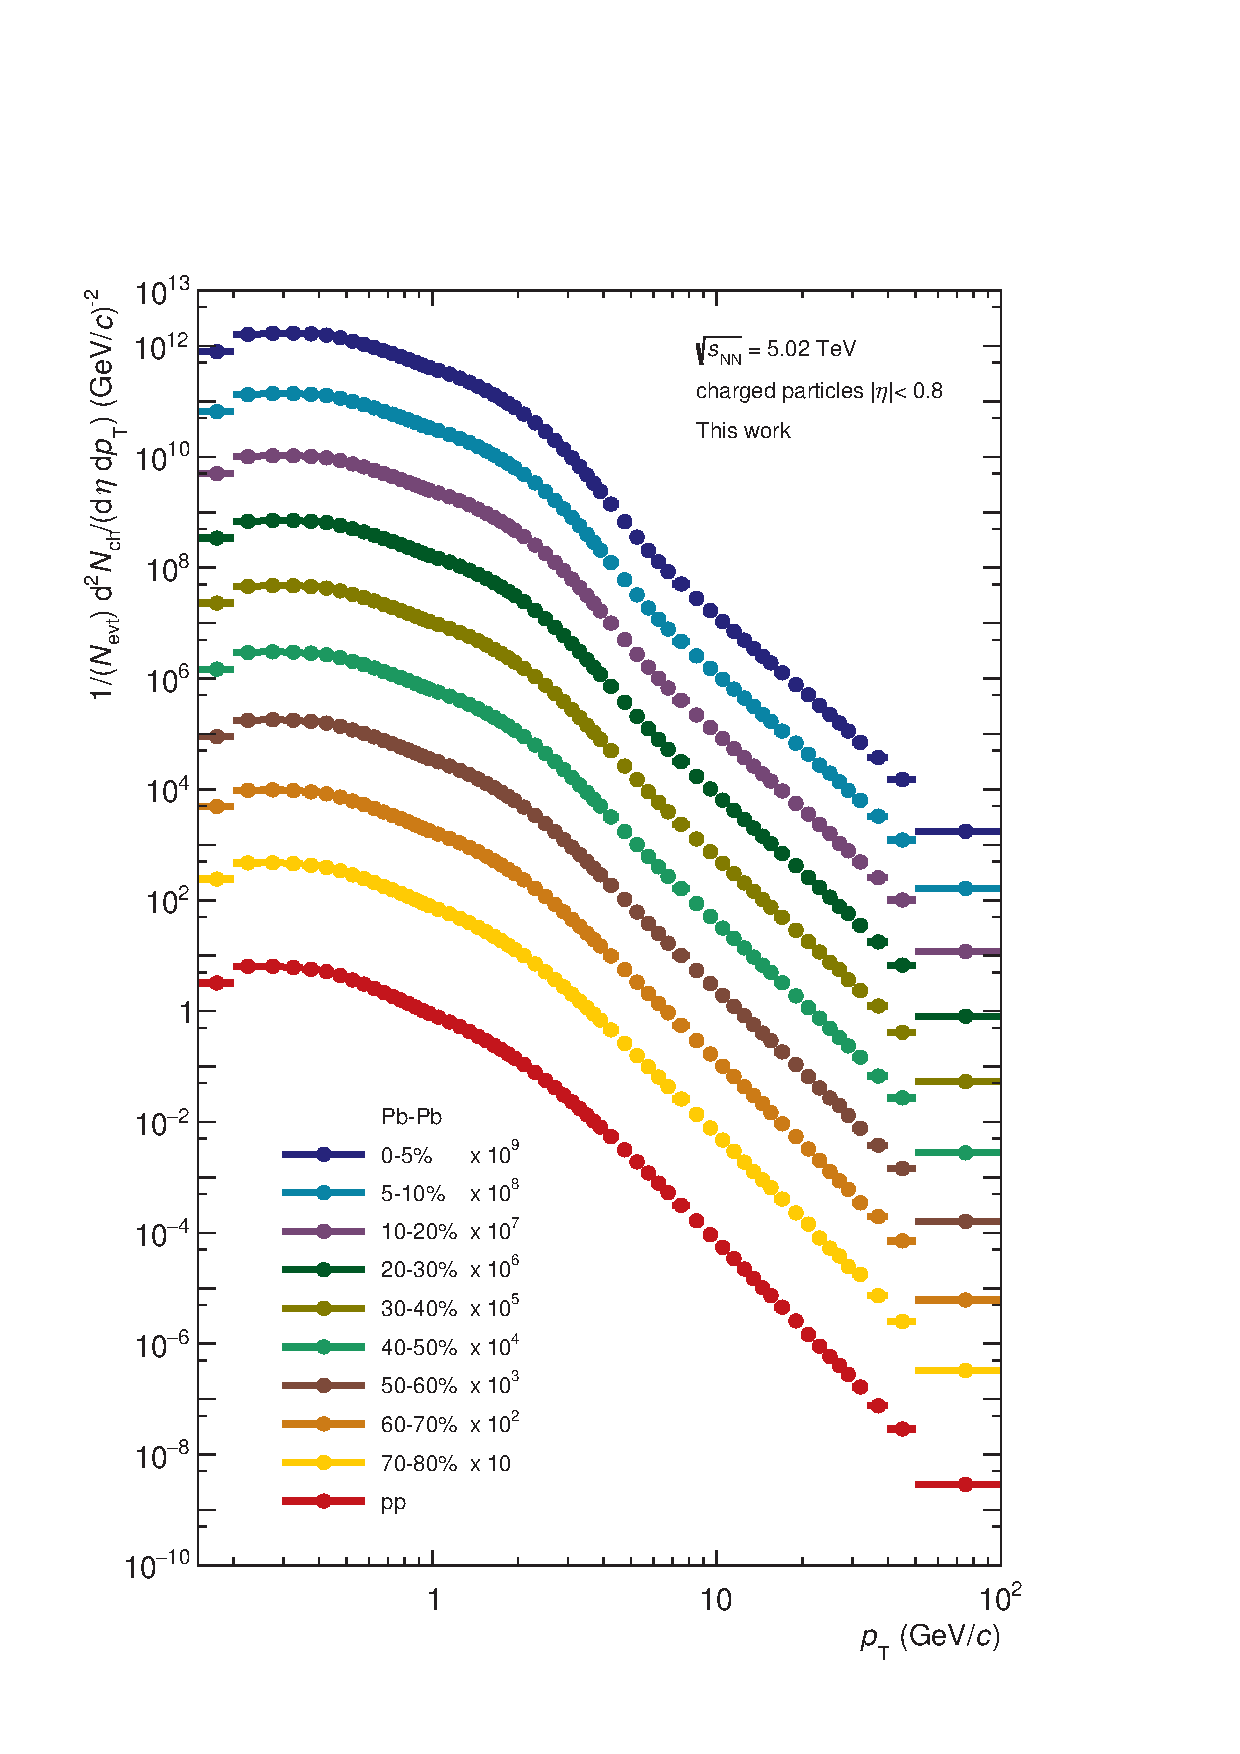
\includegraphics[width=10cm]{Plots/uncorrectedSpectra.pdf}  
\caption{Uncorrected transverse momentum distributions of primary charged particles produced in pp and Pb-Pb collisions at $\sqrt{s_\text{NN}} = 5.02$ TeV. The latter are divided into nine centrality classes. The \pt spectra of Pb-Pb collisions are scaled for a better visibility. }
\label{uncorrSpec}
\end{figure}
In Figure \ref{uncorrSpec}, the uncorrected \pt dependent distributions of the produced charged particles in pp and Pb-Pb are shown after implementing the event and track selection. In the case of heavy-ion collisions, the \pt distributions are divided into nine centrality classes. The vertical error bars represent the statistical uncertainties.\\
These \pt distributions are affected by several detector effects that must be corrected. To this end, most of the corrections are implemented using information provided by MC simulations. In addition, data-driven approaches are used to correct for imperfections of these simulations. \\
Two groups of corrections can be defined according to the level at which they operate: 
\begin{itemize}
\item corrections which operate at event-level and, as a result, influence the shift of the spectrum.
\item corrections which affect the tracks and, therefore, are \pt dependent. This group consequently conditions the shape of the spectrum.
\end{itemize}
In the following sections, the corrections applied to the \pt spectra and the analysis strategies used for their implementation will be discussed.
\subsection{Overall normalization}
\label{Norm}
\begin{table}[H]
\centering
\renewcommand{\arraystretch}{1.5}
\begin{tabular}{|c|c|}
\toprule
\rowcolor{headerBlue}  \textbf{Trigger} $\boldsymbol \epsilon_\text{Trig}$ &  \textbf{Vertex reconstruction} $\boldsymbol \epsilon_\text{Vz}$\\
\hline
75.25\%	&	98.48\%		 \\
\bottomrule
\end{tabular}
\caption{Trigger and event vertex reconstruction efficiencies for pp collisions at $\sqrt{s} = 5.02$ TeV recorded with ALICE in 2017.}
\label{tab:effs}
\end{table} 
The number events of $N_\text{ev}^\text{rec}$ that passed the selection criteria and which is used for the normalization of the \pt distributions does not include some inelastic events that were not triggered or reconstructed. These two phenomena are corrected by means of the so-called trigger efficiency $\epsilon_\text{Trig}$ and the vertex reconstruction $\epsilon_\text{Vz}$ efficiency:
\begin{equation}
N_\text{ev}^\text{rec} = N_\text{INEL}\cdot \epsilon_\text{Trig} \cdot \epsilon_\text{Vz}
\end{equation}
where $N_\text{INEL}$ represents the true number of inelastic events. In heavy-ion collisions, both trigger and vertex reconstruction efficiency have been observed to be unity in the studied centrality interval 0-80\% (cite mknichel/Pb-Pb papers). However, the bias is particularly notable in pp collisions. The determination of the respective efficiencies in pp collisions, described below, is therefore required.
\subsubsection{Trigger efficiency}
%cite ALICE 2017 luminosity determination for pp collisions at
%cite vdM:http://cds.cern.ch/record/296752/files/196800064.pdf
%cite value vis. cross section: https://twiki.cern.ch/twiki/bin/viewauth/ALICE/EventNormalization
%cite MC glauber predictions: https://arxiv.org/pdf/1710.07098.pdf
The MB condition of the ALICE trigger system is able to measure a significant percentage of the total inelastic cross section, yet this measurement is limited due to the efficiency of the trigger $\epsilon_\text{Trig}$. This efficiency connects the visible and the total inelastic cross section as follows:
\begin{equation}
\epsilon_\text{Trig}  =  \dfrac{\sigma_\text{vis}}{\sigma_\text{INEL}} 
\label{effTrig}
\end{equation}
For each data taking period, the visible cross section is measured by determining the luminosity of the experiment, a quantity that evaluates the number of particle collisions and which is measured in events per time per area. To this purpose, a technique called van-der-Meer scan is used, in which the two particle beams are displaced with respect to each other in the transverse directions and the rate of interactions is monitored as a function of this displacement. The ratio of the head-on rate to the luminosity corresponds then to the desired visible cross section (cite S. vdM). In the studied pp collisions collected in 2017 at $\sqrt{s} = 5.02$ TeV, the visible cross section amounts to $\sigma_\text{vis} = 50.87 \pm 1.07$ mb (cite value). \\
The total inelastic cross section $\sigma_\text{INEL}$ has not been measured in pp collisions at $\sqrt{s} = 5.02$ TeV. However, a Monte Carlo Glauber model is able to predict by means of a data-driven parametrization the value of $\sigma_\text{INEL}$ as function of the center-of-mass energy 	(cite MC Glauber paper). Here, experimental values from several collaborations are utilized as input. According to the prediction, the total inelastic cross section at $\sqrt{s} = 5.02$ TeV is $\sigma_\text{INEL} = 67.6 \pm 0.6$ mb (cite value). The resulting trigger efficiency is shown in Table \ref{tab:effs}.
\subsubsection{Vertex reconstruction efficiency}
The vertex reconstruction efficiency $\epsilon_\text{Vz}$ can be defined as follows:
\begin{equation}
\epsilon_\text{Vz} = \dfrac{N_\text{Vtx}}{N_\text{Trig}} 
\end{equation}
where $N_\text{Vtx}$ is the number of events for which a vertex was reconstructed and $N_\text{Trig}$ is the total number of triggered events. Both values were determined before the event selection. The resulting efficiency can be found once again in Table \ref{tab:effs}.
\subsubsection{Signal loss correction}
\begin{figure}[tb!]
\centering
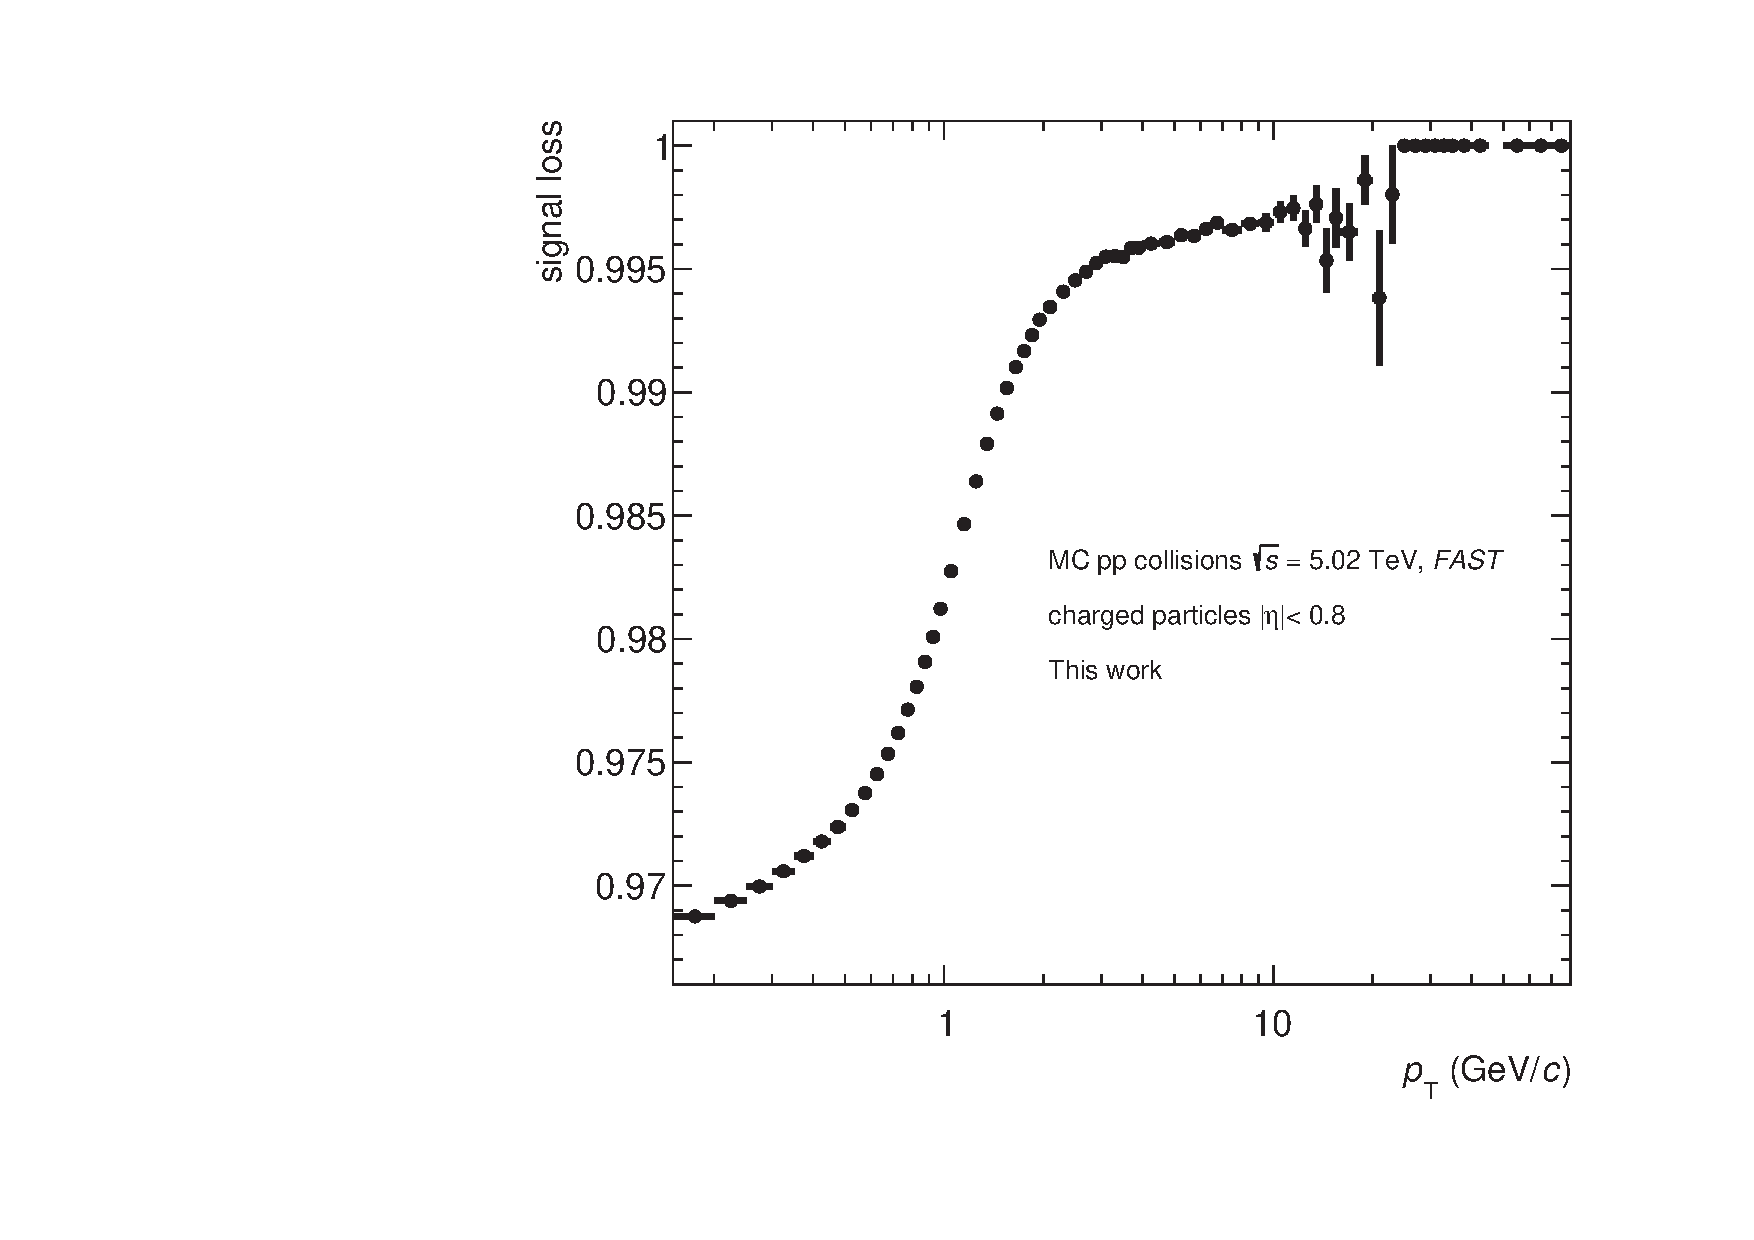
\includegraphics[width=12cm]{Plots/signalLossFAST.pdf}  
\caption{Signal loss for pp collisions.}
\label{sigLoss}
\end{figure}
%find reference
A fraction of the inelastic events is missing due to the trigger and the vertex reconstruction efficiency and it must be thus restored. However, this correction has to be combined with a complementary correction at track-level in order to regain the tracks from missing events. This is achieved using the MC production to compare the distribution of primary tracks generated from inelastic events within the vertex cut $|V_z| < 10$ cm before and after they undergo the event selection:
\begin{equation}
\chi_\text{sig loss}(p_\text{T}) = \dfrac{(\text{d}N/\text{d}p_\text{T})_\text{Generated}^\text{After event selection}}{(\text{d}N/\text{d}p_\text{T})_\text{Generated}^\text{True INEL>0, |Vz|<10 cm}}
\end{equation}
As result, the \pt dependent distribution of the signal loss $\chi(p_\text{T})$ is shown in Figure \ref{sigLoss}. The effect is more pronounced at low $p_\text{T}$, where it amounts to about 3\%. The signal loss decreases, becoming negligible above 10 GeV/$c$. The required correction is implemented by scaling the \pt spectrum in each \pt interval with the inverse of the corresponding value of the signal loss.
\subsection{Tracking efficiency and acceptance}
\begin{figure}[tb!]
\centering
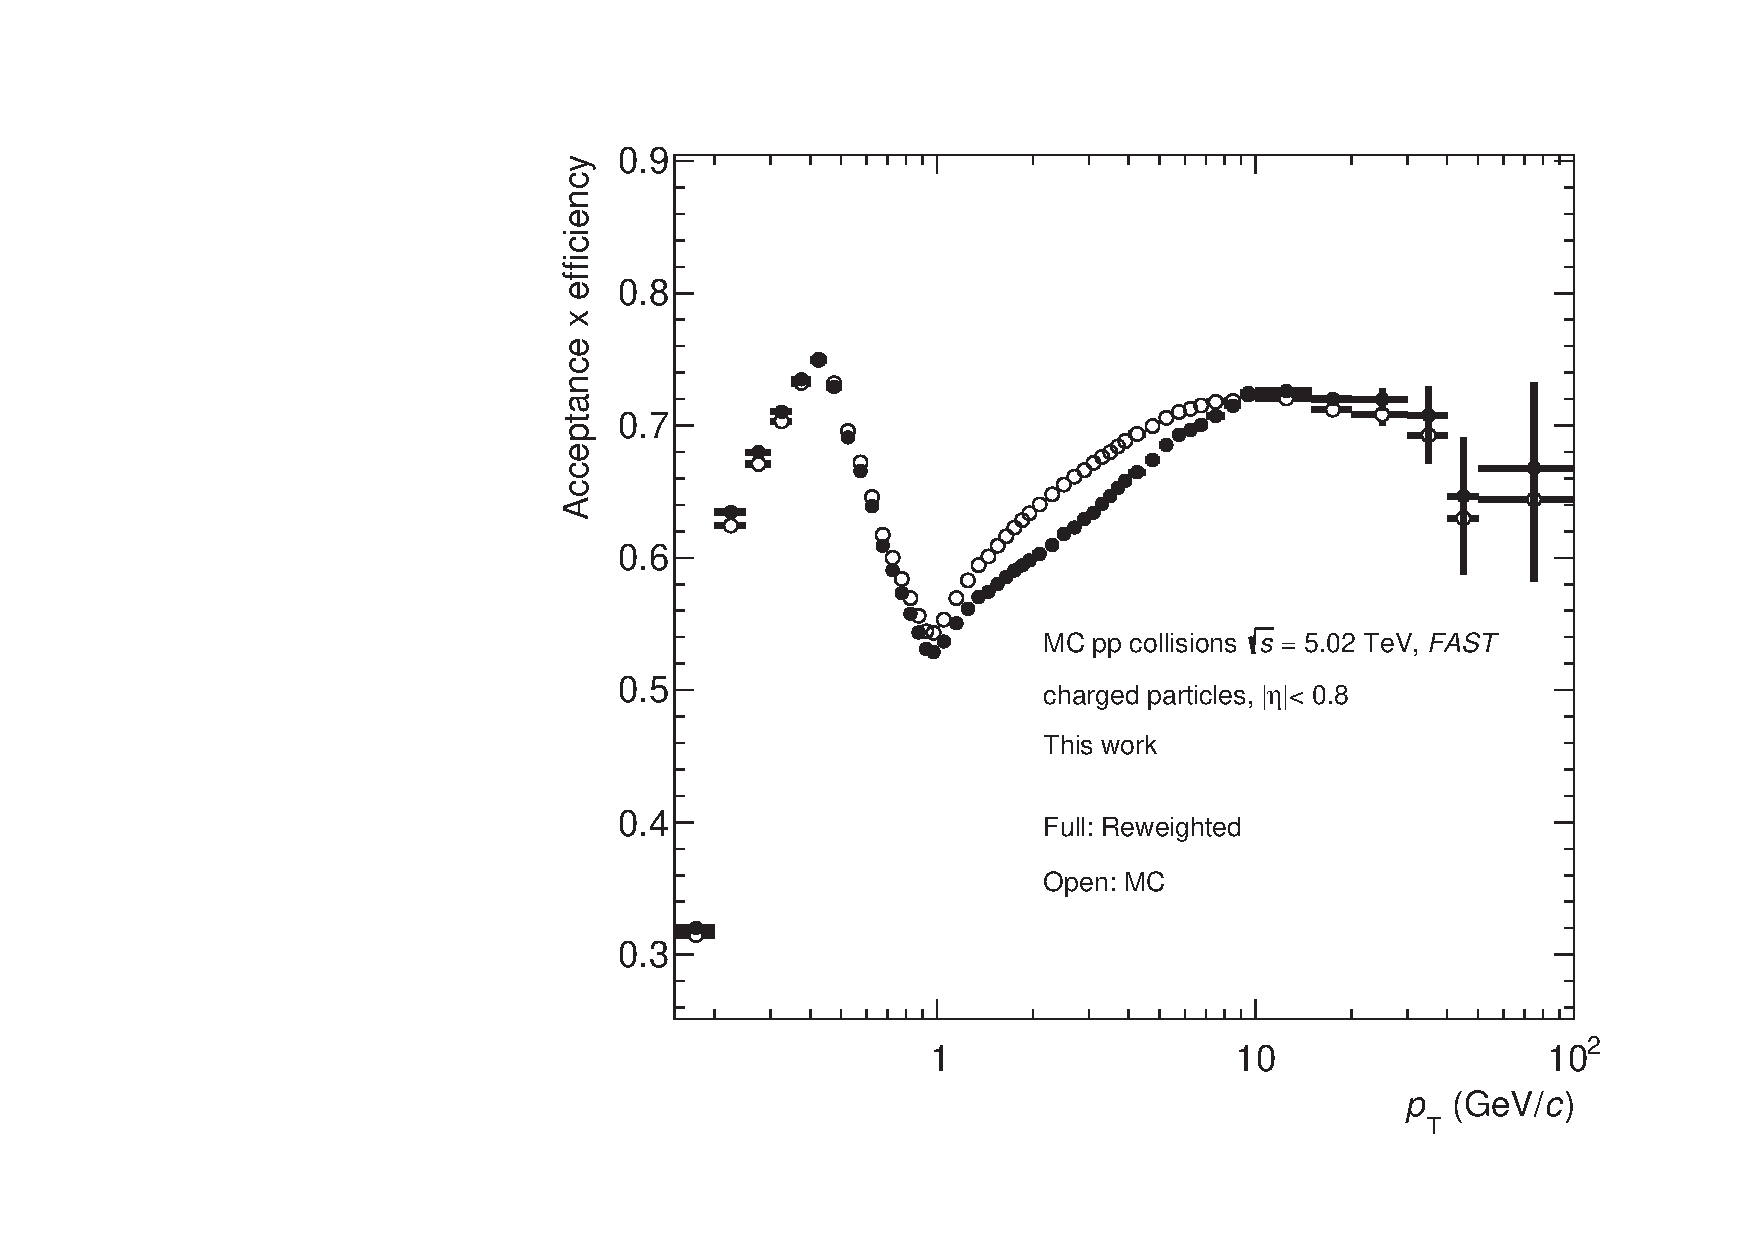
\includegraphics[width=12cm]{Plots/trckEffpp.pdf}  
\caption{Acceptance and tracking efficiency as function of the transverse momentum for pp collisions obtained from MC simulations.}
\label{trckEffpp}
\end{figure}
The TPC-ITS detector system is able to measure most of the tracks that cross the detector volume. However, the reconstruction algorithm is sometimes unable to detect a track or to reconstruct it correctly which then causes it to be discarded by the track selection. In fact, tracks are measured with a probability. Moreover, the acceptance coverage of the detector, defined by the kinematic range of $0 \leq \phi \leq 2\pi$, $|\eta| < 0.8$ and \pt $> 0.15$ GeV/$c$, affects also the measurement of charged particles. \\
The tracking efficiency and acceptance can be summarized in an overall detection efficiency $\epsilon$ for the reconstruction of tracks which depends on transverse momentum \pt. The implementation of the corresponding correction will thus affect the shape of the \pt distributions. The \pt dependent efficiency is calculated using the MC simulations as the ratio of reconstructed primary tracks that survive the track selection $N_\text{rec}^\text{MC}$ to generated primary charged-particles $N_\text{gen}^\text{MC}$: 
\begin{equation}
\epsilon(p_\text{T}) = \dfrac{N_\text{prim,rec}^\text{MC}(p_\text{T})}{N_\text{prim,gen}^\text{MC}(p_\text{T})} 
\label{trckEffEq}
\end{equation}
For the correction, the inverse of the overall efficiency is applied as a multiplicative factor on the \pt spectra.\\
The overall efficiency also depends on the type of particle measured. This requires the implementation of a complementary correction, explained later on, which scales the overall efficiency by means of the relative abundance of each particle type (cite Patricks thesis).\\
\begin{figure}[tb!]
\centering
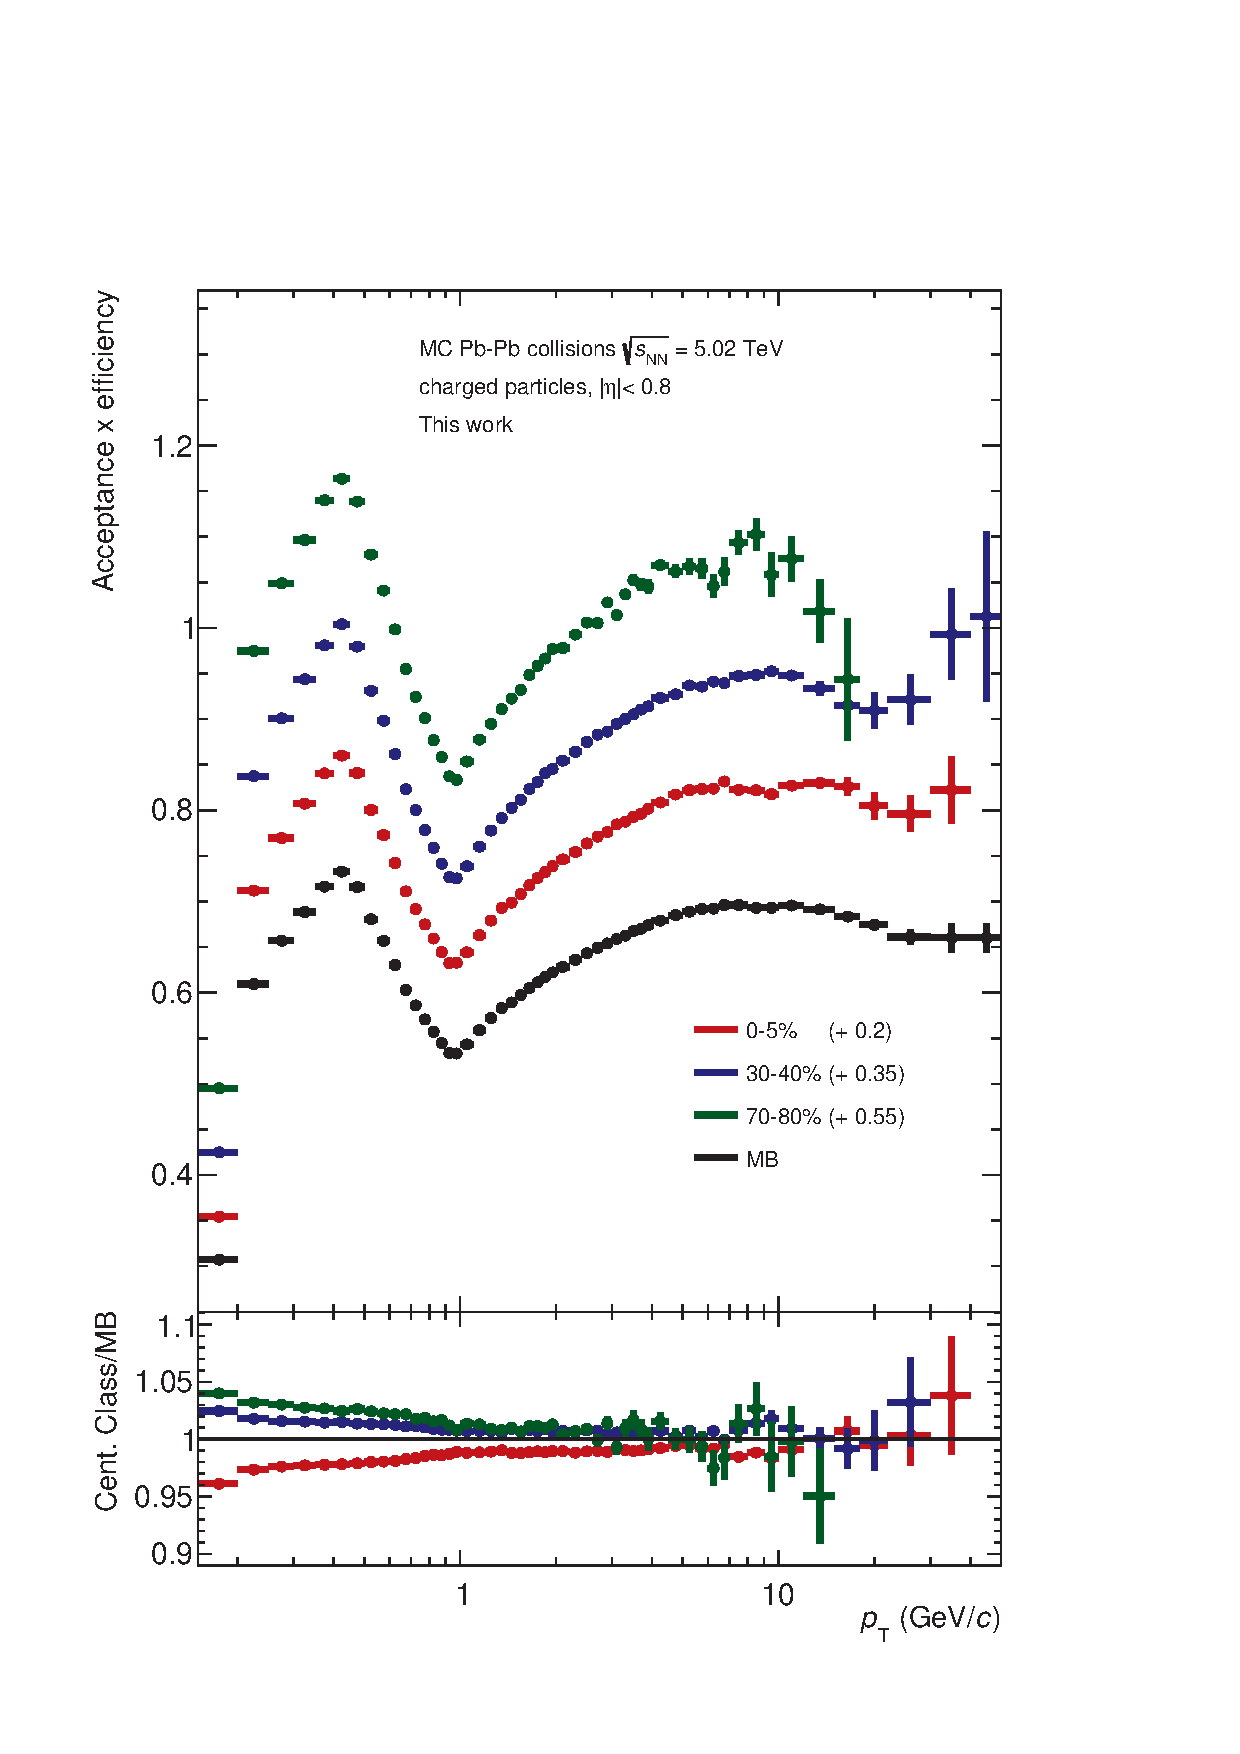
\includegraphics[width=12cm]{Plots/trckEffPbPb1.pdf}  
\caption{Tracking efficiency as function of the transverse momentum for MB, central, semi-central and peripheral Pb-Pb collisions obtained from MC simulations. An offset value is added to the efficiencies for a better visibility. In the bottom panel, the ratio of the individual efficiencies to the MB efficiency is shown. Data points with very large statistical deviations are excluded.}
\label{trckEffPbPb1}
\end{figure}
\begin{table}[tb!]
\centering
\renewcommand{\arraystretch}{1.5}
\begin{tabular}{|c|c|}
\toprule
\rowcolor{headerBlue} \textbf{Centrality class} &  \textbf{Scaling factor}\\
\midrule
0-5\%	&	0.980	 \\
5-10\%	&	0.995	 \\
10-20\%	&	1.000	 \\
20-30\%	&	1.004	 \\
30-40\%	&	1.007	 \\
40-50\%	&	1.009	 \\
50-60\%	&	1.010	 \\
60-70\%	&	1.011	 \\
70-80\%	&	1.010	 \\
\bottomrule
\end{tabular}
\caption{Scaling factors obtained from the parametrization of the ratios in Figure \ref{trckEffPbPb1}.}
\label{tab:ScalingFactors}
\end{table} 
\hspace{-0.3cm} In Figure \ref{trckEffpp}, the overall efficiency as function of \pt is shown for pp collisions. Here, the efficiency amounts to a value between 54\% and 75\% over the entire \pt range. At low $p_\text{T}$, below 0.4 GeV/$c$, there is a rapid growth of the efficiency which can be explained by the increasing radii of the particle trajectories making it more likely for the track to fulfil the strict selection criteria. After reaching the maximum, the curve drops quickly and hits its minimum around 1 GeV/$c$. This slump is caused mainly by the track length cut listed in Table \ref{tab:Cuts} which aims for a selection of tracks that fulfil a minimal geometric length within the fiducial detector volume. The tracks in the $p_\text{T}$-range of the slump tend to cross the TPC boundaries so that they are less likely to be selected. Following this, the distribution increases asymptotically due to the acceptance restrictions of the detector up to reaching a plateau (cite paper). The overall efficiency is assumed to be constant for $p_\text{T} \geq 40$ GeV/$c$ in order to reduce statistical fluctuations. \\
\begin{figure}[tb!]
\centering
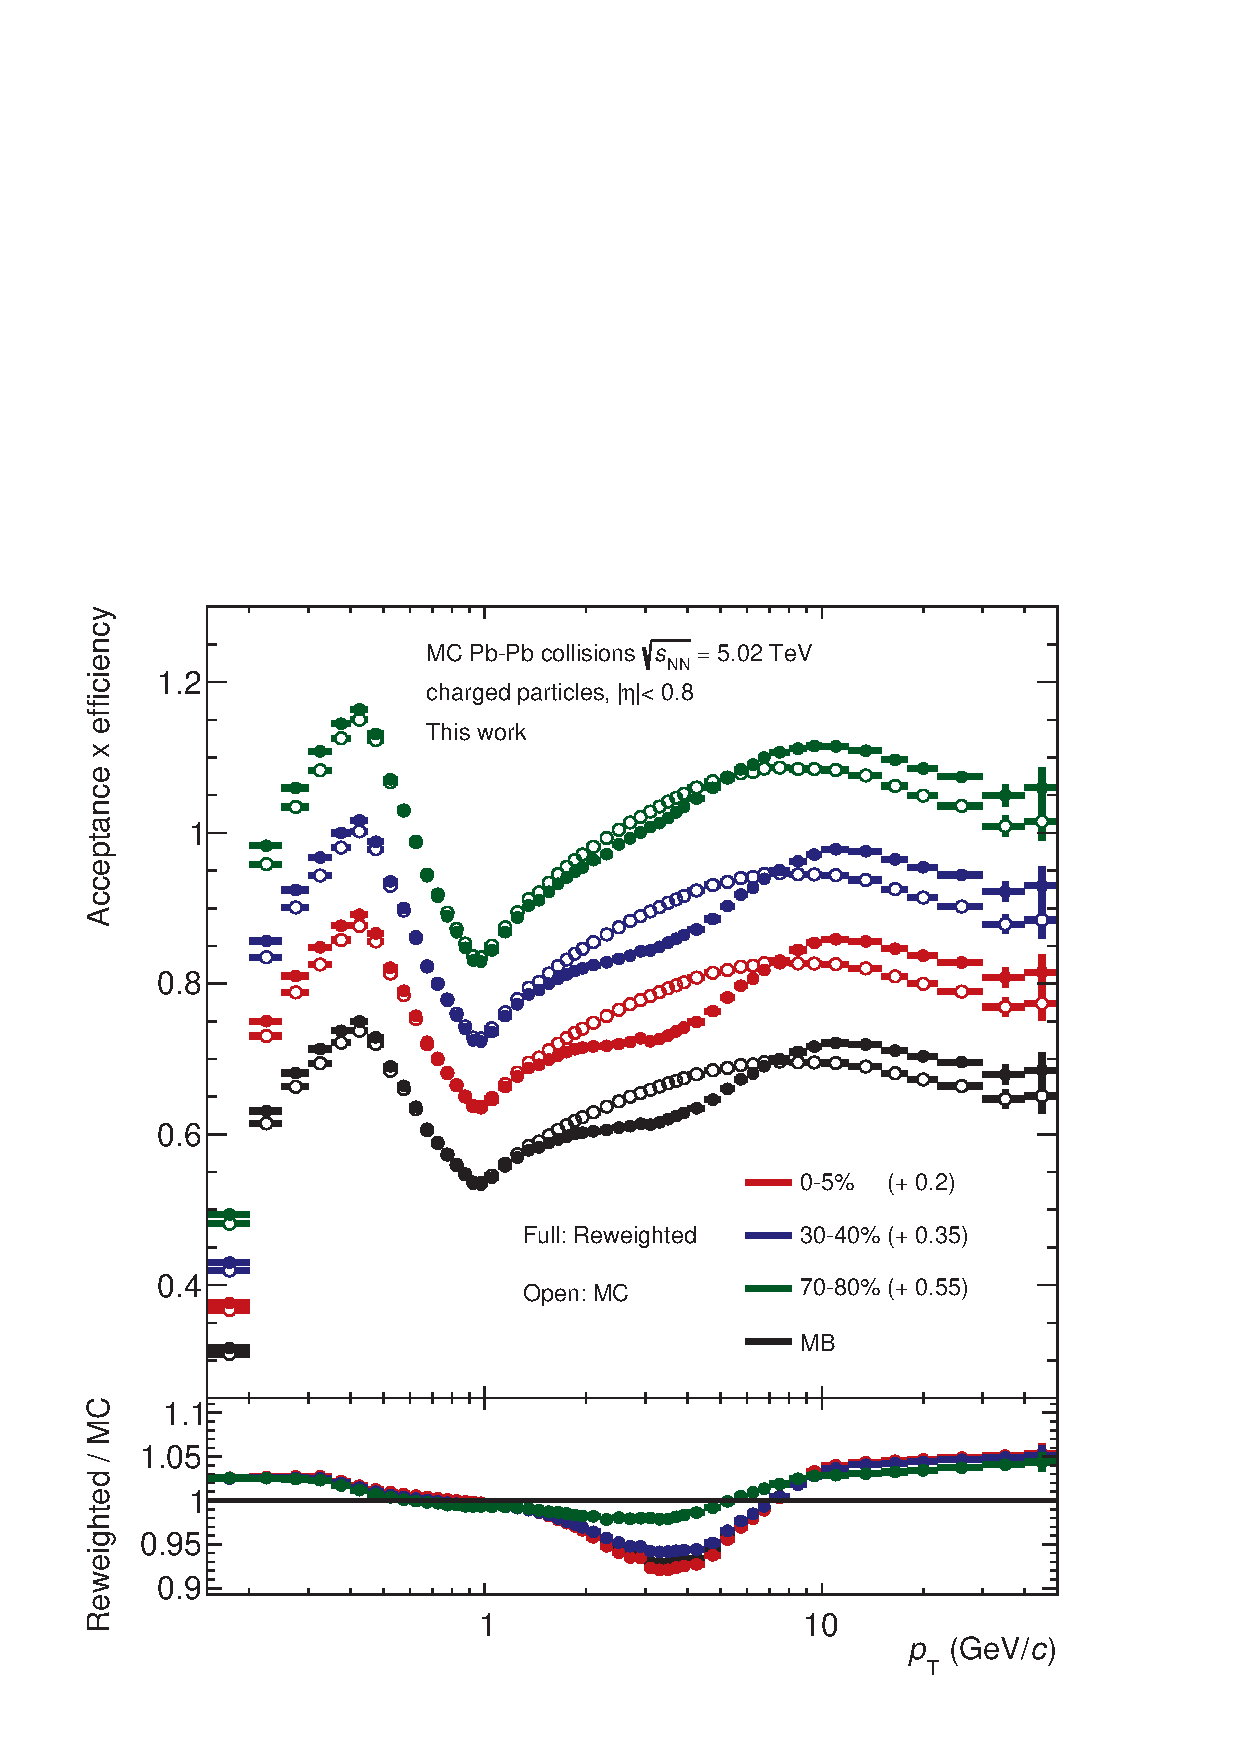
\includegraphics[width=12cm]{Plots/trckEffPbPb2.pdf}  
\caption{Tracking efficiency as function of the transverse momentum for MB, central, semi-central and peripheral Pb-Pb collisions obtained from the scaling of the distributions in Figure \ref{trckEffPbPb1} using the values listed in Table \ref{tab:ScalingFactors}.  An offset value is added to the efficiencies for a better visibility.}
\label{trckEffPbPb2}
\end{figure}
\hspace{-0.3cm} This same behavior is also observed in Pb-Pb collisions analysed in this thesis as illustrated in Figure \ref{trckEffPbPb1}, which shows the overall efficiency as function of \pt for MB, central ($0-5$\%), semi-central ($30-40$\%) and peripheral ($70-80$\%) collisions. The tracking efficiency decreases with this centrality. As also observed in this figure, the high \pt range of the centrality-dependent efficiencies is dominated by very large statistical fluctuations. To avoid subsequent distortions in the \pt distributions, the ratios of the individual efficiencies to the MB efficiency, illustrated in the bottom panel, are parametrized from a \pt of 1.5 GeV/$c$ with a constant function. The obtained factors, summarized in Table \ref{tab:ScalingFactors}, are used to scale the MB tracking efficiency for \pt > 1.5 GeV/$c$, while the original efficiencies are used below this range. As result,  the distributions obtained using this approach are represented in \ref{trckEffPbPb2} with open marks. 
\subsubsection{Particle composition correction}
%https://pdg.lbl.gov/2020/citation.html
\begin{figure}[tb!]
\centering
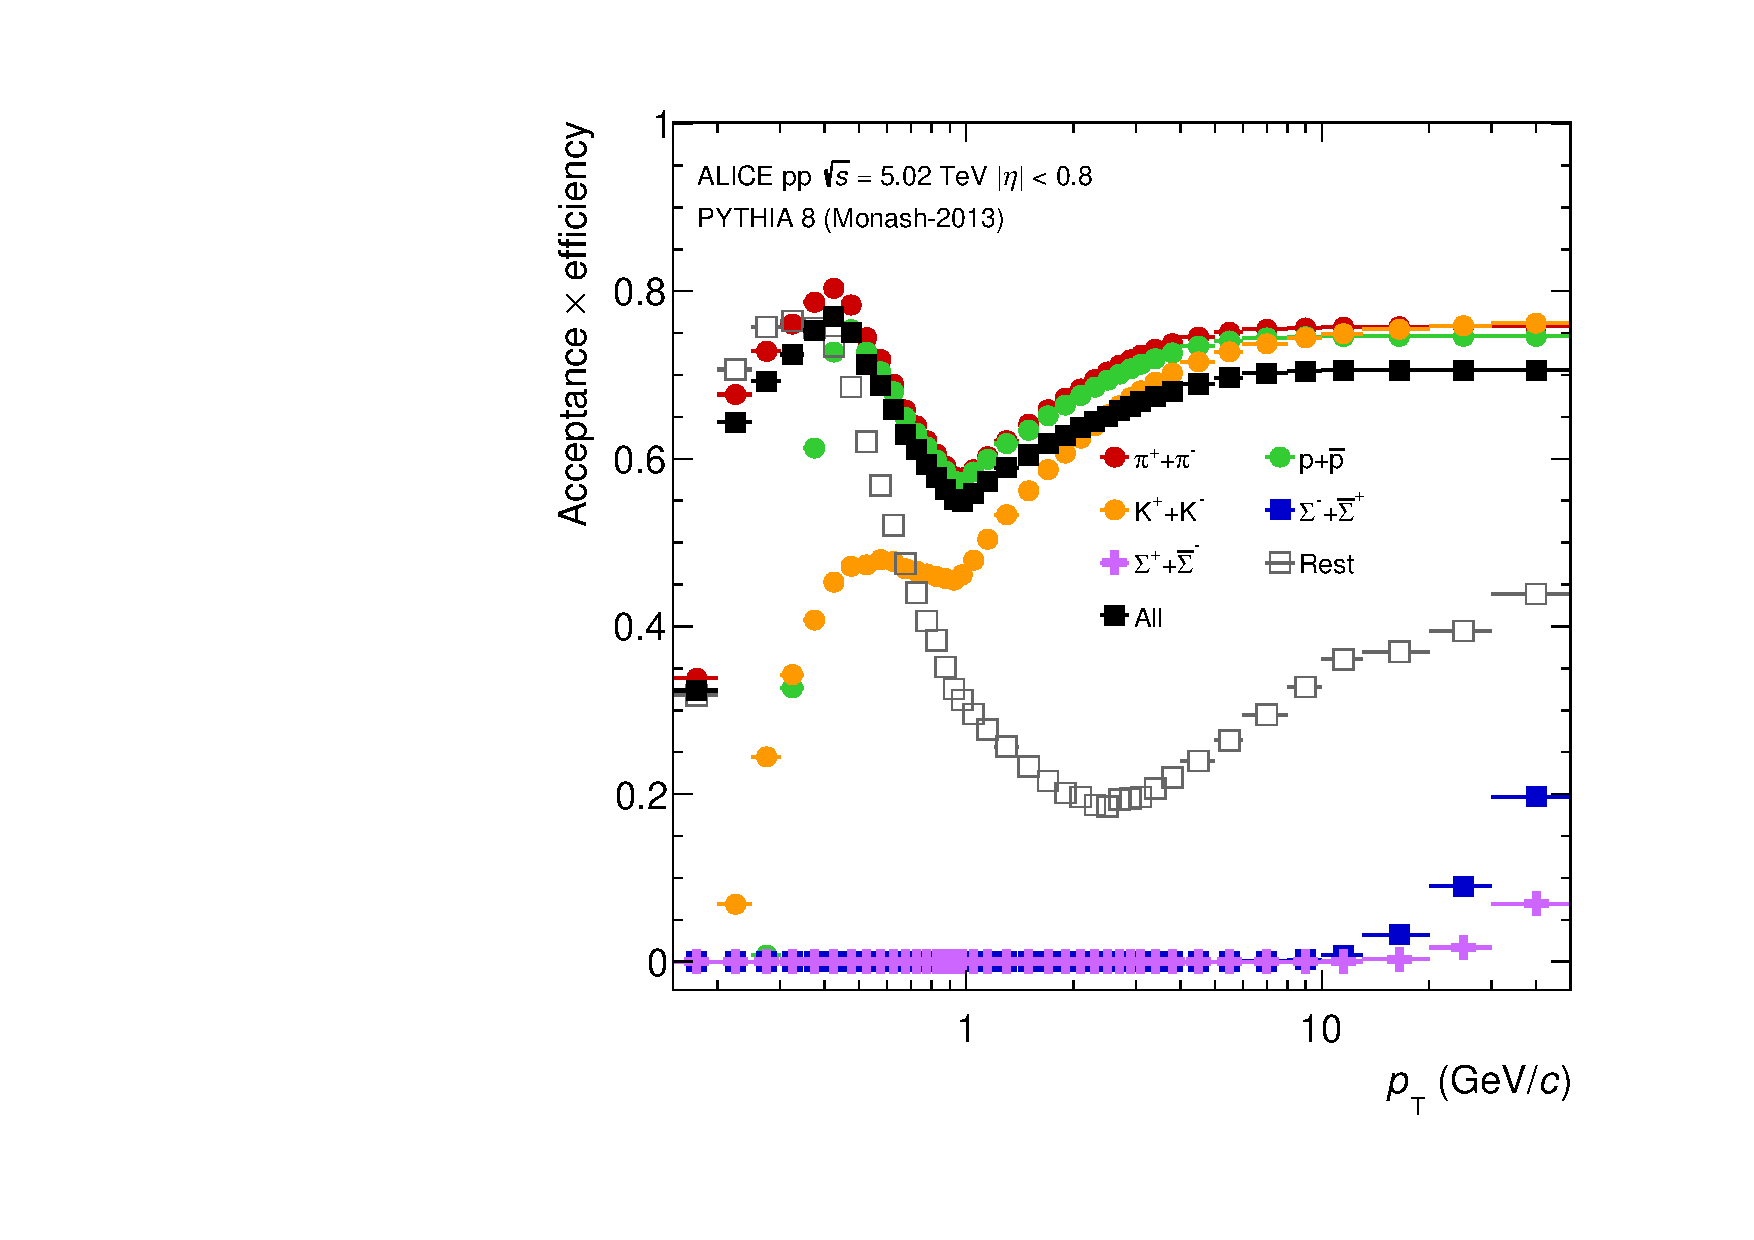
\includegraphics[width=0.495\textwidth]{Plots/5TeVMonash13_TrkEff_without-91972.pdf}  
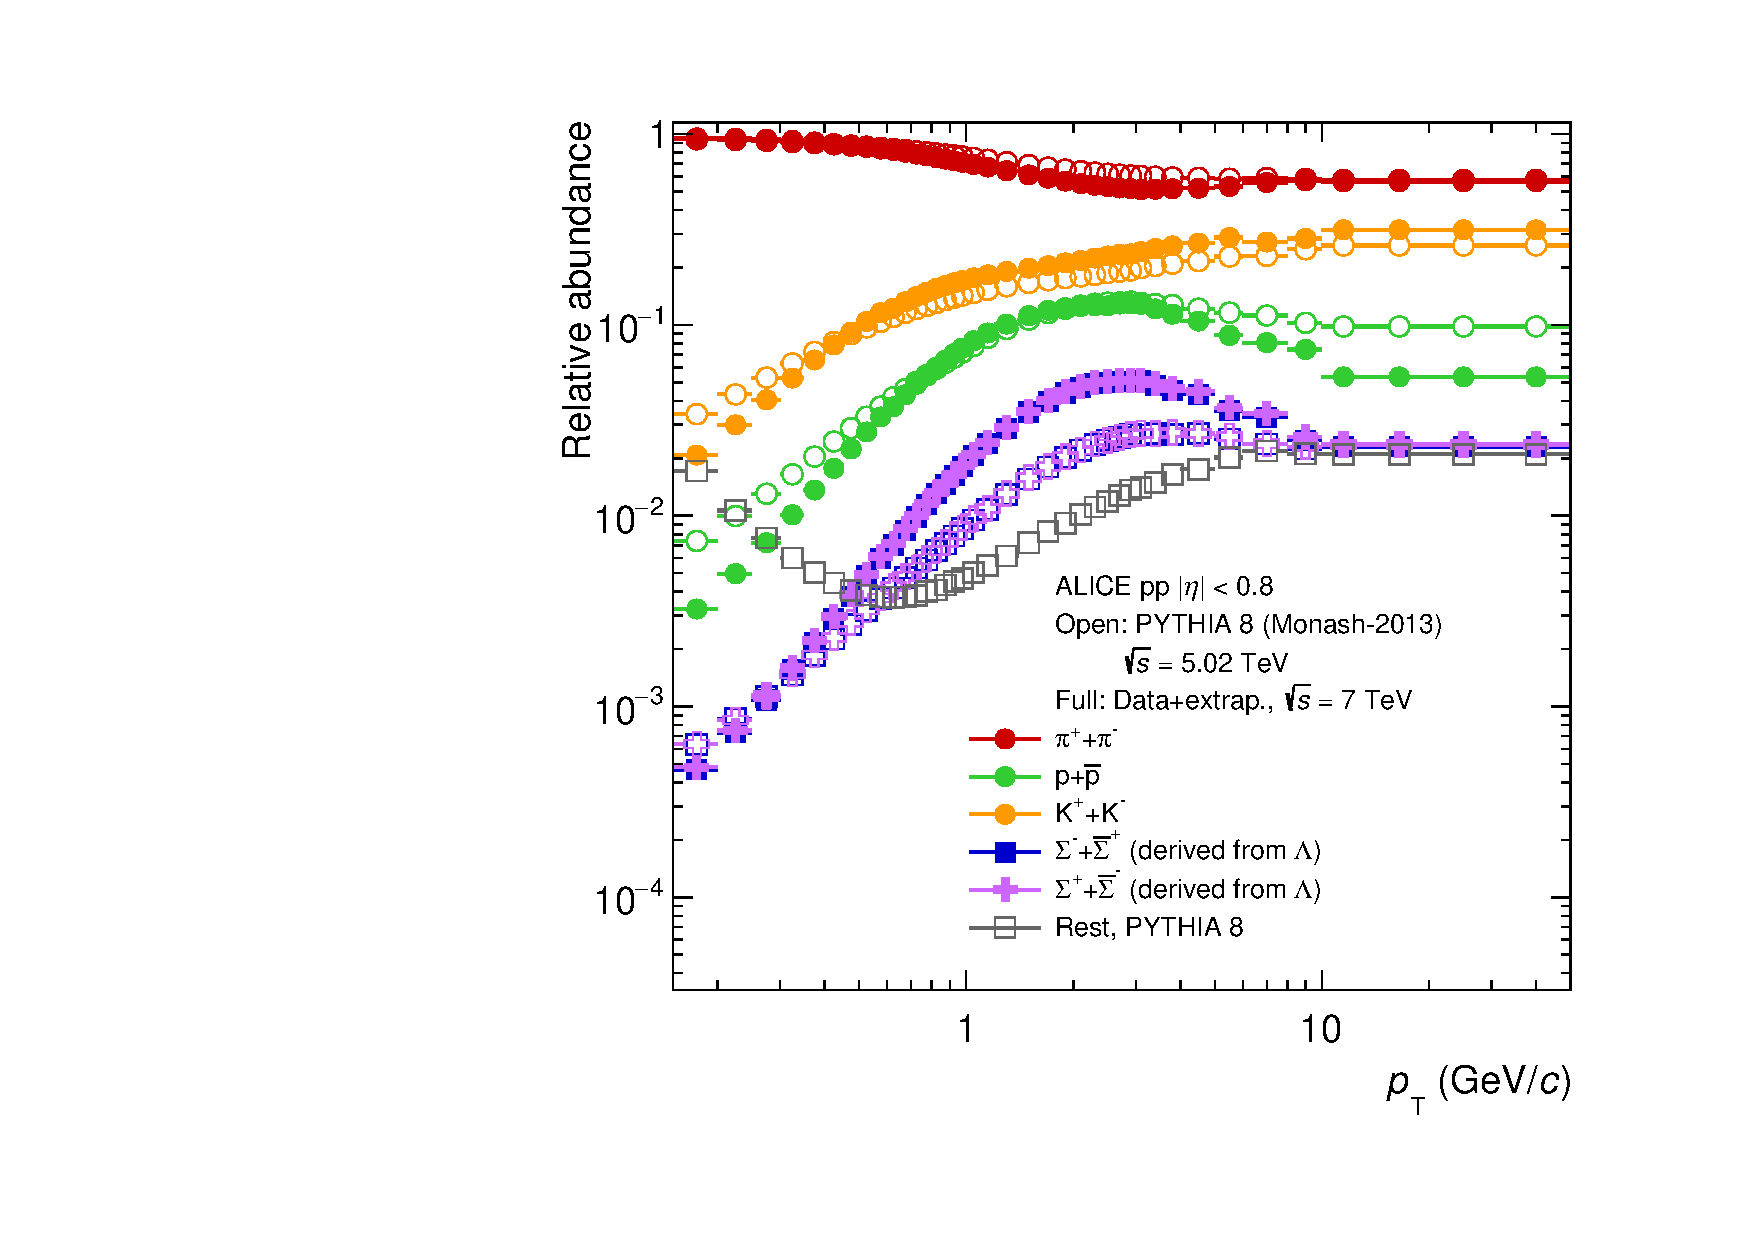
\includegraphics[width=0.495\textwidth]{Plots/5TeVMonash13_Abundances-91973.pdf}  
\caption{\textbf{Left: }Tracking efficiencies as function of the transverse momentum for different particle species obtained with a PYTHIA (Monash 13) simulation of pp collisions at $\sqrt{s} = 5.02$ TeV. \textbf{Right:} Relative particle abundances as function of the transverse momentum in data (full symbols,  $\sqrt{s} = 7$ TeV) and in MC (open symbols,  $\sqrt{s} = 5.02$ TeV) (cite paper).}
\label{trckEffParticles}
\end{figure}
Among the primary charged particles that compound the studied sample, a disparity in terms of the lifetime is observed. For instance, the pions ($\pi^{\pm}$), the most frequent particle type produced in particle collisions, can travel in average $7.8\text{ m}$ within their lifetime, whereas the sigma baryons ($\Sigma^{\pm}$) have a decay length of only $2.4\text{ cm}$ (cite pdg booklet). As consequence, some particles are more likely to be rejected by the track length requirement than others, which results in the tracking efficiency depending on the particle type. \\
The usage of MC event generators, such as PYTHIA or HIJING, allows to obtain the tracking efficiencies for different particle species as shown in the left panel of Figure \ref{trckEffParticles}. Here, results from  an analysis of the particle dependent efficiency for pp collisions at $\sqrt{s} = 5.02$ TeV are presented (cite paper). As shown in the Figure, the dependence sof the efficiency on the particle type is strong, especially below $1$ GeV/$c$. In Pb-Pb collisions, similar effects are observed as can be seen in Appendix \ref{TrkEffApp}. Because of these similarities, the correction procedure is only shown for pp collisions, although an analogous procedure is also implemented for Pb-Pb collisions.\\
Considering the particle type dependence of the efficiency, the abundance of each particle plays an important role and must therefore be reflected in the correction. However, MC event generators have limitations in the description of the particle production, especially regarding strange particles (cite 38,39 paper). As consequence, the efficiency is considerably affected by this underestimation and a correction by means of a re-weighting of the efficiency with the relative abundance of each particle type is implemented. The right plot of Figure \ref{trckEffParticles} shows the relative abundances measured in pp collisions recorded by ALICE at $\sqrt{s} = 7$ TeV. This center-of-mass energy will be used since no significant energy dependence has been observed experimentally and because of the lack of experimental data at the energy studied in this work (cite Patrick). The distributions used in this thesis were calculated by the cited analysis using a data-driven procedure and correspond to he same distributions used in the previous ALICE measurement of nuclear modification factors (cite paper).\\
In summary, the overall efficiency for inclusive particles should be understood as a weighted superposition of the individual efficiencies for each particle type with the relative particle abundances. After applying this reweighting on the distributions represented in Figures \ref{trckEffpp} and \ref{trckEffPbPb2} with open symbols, the corrected tracking efficiencies for inclusive particle are obtained and shown in these same figures with full markers. These distributions are utilized ultimately to correct the \pt distributions. 
\subsection{Contamination by secondary particles}
The selection procedure described in Section \ref{TrackSelection} aims to reduce the contamination of the measured track sample with secondary particles. Nevertheless, a small amount of these particles persists in it. This remnant originates from weak decays of kaons, $\Lambda$ baryons and muons as well as from interactions with the detector material. The remaining fraction of secondary particles has to be subtracted from the raw \pt distributions to ensure purity of the data.\\
The estimation of contamination by secondaries is carried out using the MC productions anchored to the analysed data periods. In Figure \ref{SecCont}, the result of these estimations can be seen with open markers for pp collisions as well as for MB, central ($0-5$\%), semi-central ($30-40$\%) and peripheral ($70-80$\%) Pb-Pb collisions. In general, a contamination of around  $10\%$ at low \pt can be observed. The distributions then fall monotonously with increasing \pt below $1\%$ in the high \pt region. These observations are consistent with the assumption that secondaries are inclined to carry small momenta since they correspond essentially to fractions of the momenta of the mother particles. In Pb-Pb collisions, the contamination depends on the centrality. At low $p_\text{T}$, the contamination in central collisions ($0-5$\%) amounts to almost twice as much as the contamination in the most peripheral ($70-80$\%) collisions. This is a result of an enhancement of the yield of strange particles observed in systems with high energy densities (cite here). The dependence on the centrality reduces in the high $p_\text{T}$ range.
\begin{figure}[tb!]
\centering
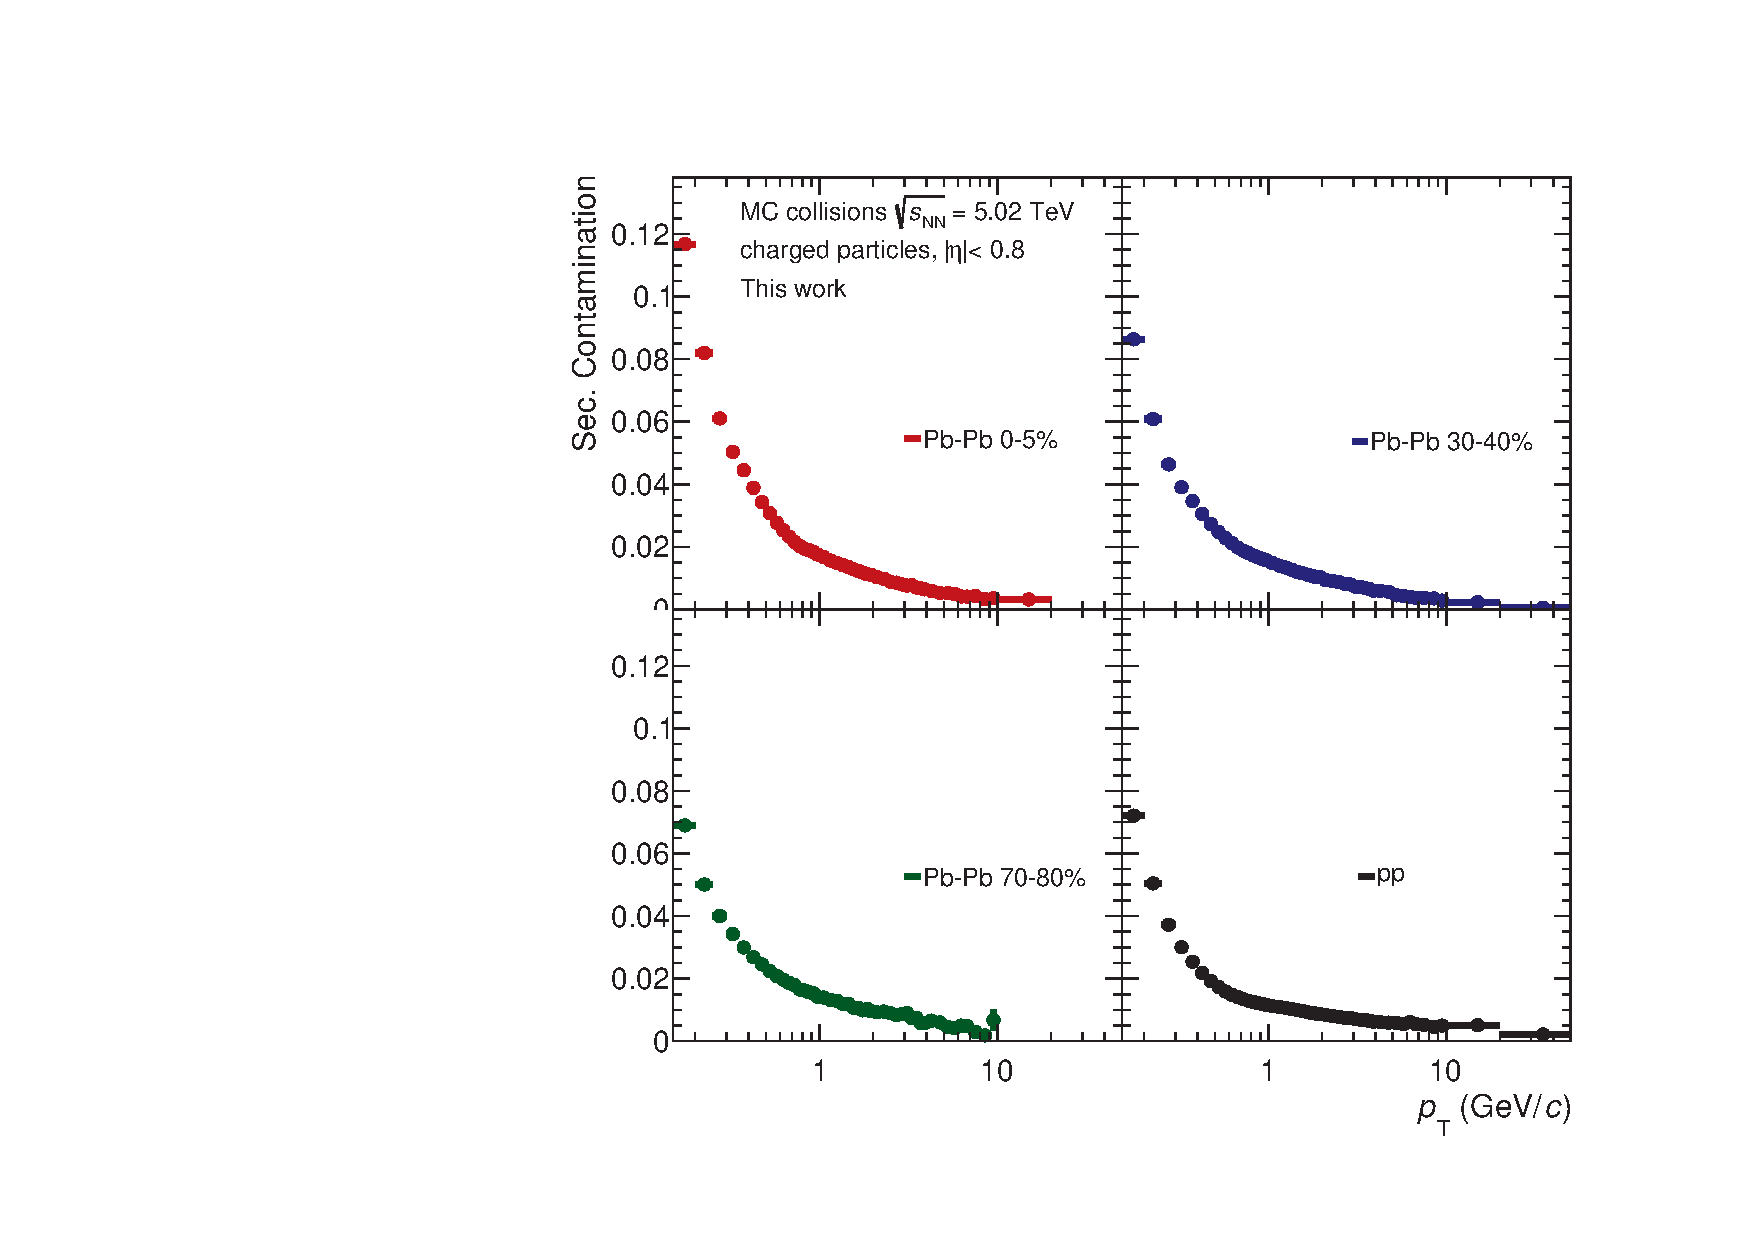
\includegraphics[width=12cm]{Plots/secCont.pdf}  
\caption{Contamination with secondary particles as function of the transverse momentum obtained from MC simulations for pp collisions as well as central, semi-central and peripheral Pb-Pb collisions. Open markers represent the secondary contamination obtained from pure MC, while the full ones correspond to the  corrected contamination.}
\label{SecCont}
\end{figure}
\subsubsection{Secondary scaling}
%cite TFractionFitter A la HMCMLL, see R. Barlow and C. Beeston, Comp. Phys. Comm. 77 (1993) 219-228, and http://www.hep.man.ac.uk/~roger/hfrac.f
\begin{figure}[tb!]
\centering
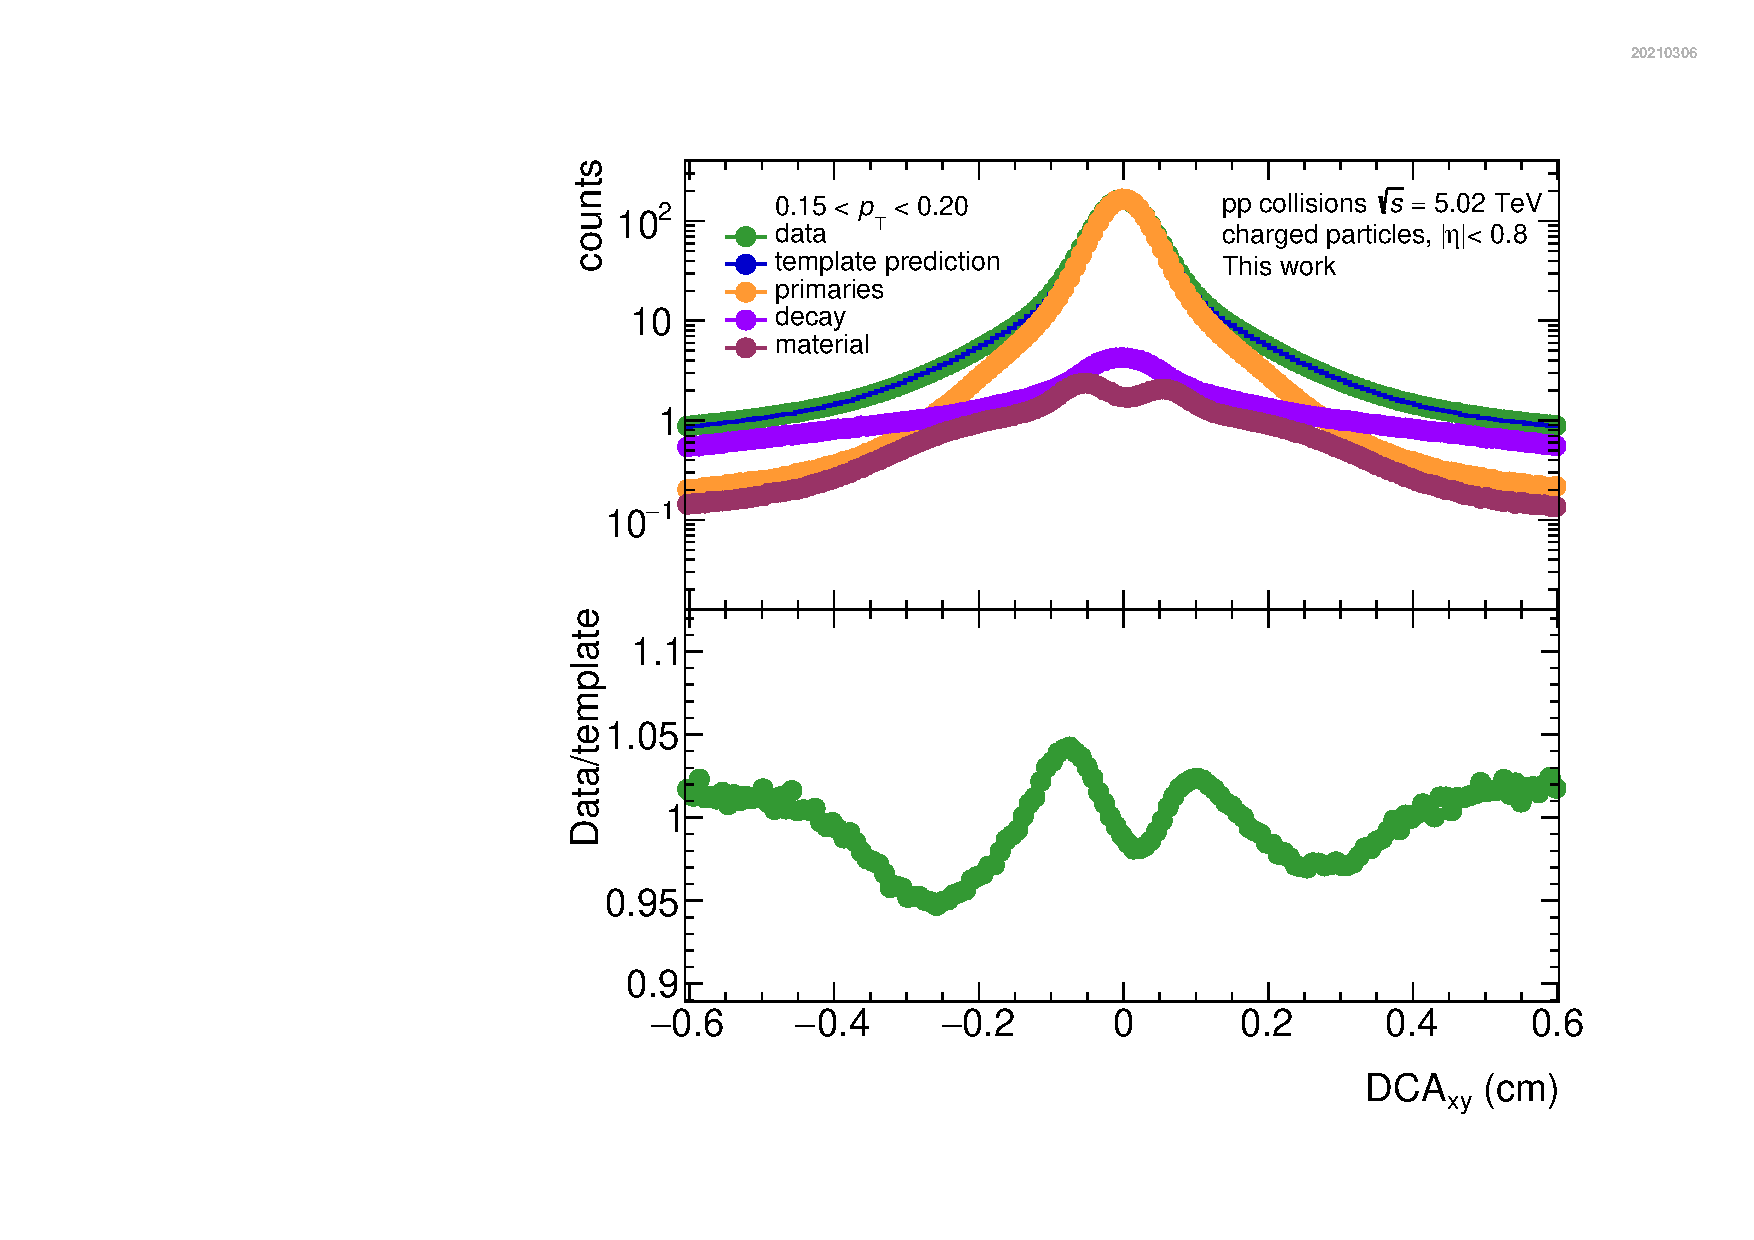
\includegraphics[width=12cm]{Plots/DCAdistributions.pdf}  
\caption{DCA$_\text{xy}$ distributions for data and MC simulations for pp collisions at $\sqrt{s} = 5.02$ TeV for the \pt range $0.15 \leq $ \pt $< 0.19$ GeV/$c$. The MC predictions correspond to primaries, secondaries from decay and secondaries from interactions in the detector material. In the bottom panel, the ratio of distribution for data to the fit resulting from the MC templates is shown.}
\label{secScaling}
\end{figure}
As stated in the previous section, MC productions underestimate the yield of strange particles. This limitation distorts the true contamination by secondaries. For this reason, the relative abundances of primary and secondary charged particles in data must be determined in order to scale the contamination correspondingly.\\
This approach must therefore be based on a property which distinguishes between primaries and secondaries. In this regard, the distance of closest approach (DCA) offers the possibility for a clear discrimination between these two groups, given that the respective DCA$_{\text{xy}}$ distributions should have distinct shapes. The differences should arise particularly in the region of the tails, where the largest DCA$_{\text{xy}}$ values are located. In this regard, the track selection must be modified in order to obtain a statistically significant result. In particular, the new track selection dispenses with the cuts on the DCA$_\text{xy}$ and on the  $\chi^2_\text{TPC-ITS}$, both of which suppress the yield of secondaries. This modification of the track selection allows to measure an amount of secondaries sufficiently large to extract scaling factors for a few intervals at low $p_\text{T}$ in the range $0.15 \leq p_\text{T} < 1.5 $ GeV/$c$.\\
In the upper panel of Figure \ref{secScaling}, the DCA$_{\text{xy}}$ distribution for pp collisions recorded by ALICE is illustrated for the \pt interval $0.15 \leq p_\text{T} < 0.2 $ GeV/$c$. In the same figure, the corresponding MC predictions of the DCA$_{\text{xy}}$ in pp collisions for primaries, secondaries from decays and secondaries originated from interactions in the detector material are represented. Primaries present a shape with a prominent peak at $0$ cm that far exceeds the small peak that characterize both distributions for secondaries. Differences are also noticeable in the tails of the distributions, where secondaries, as expected, show much broader curves. The data distribution clearly resembles the shape for primary particles since these dominate the particle production. These observations can be extended for the rest of $p_\text{T}$ intervals and also for the case of Pb-Pb collisions as it can be seen in the corresponding Figures in the Appendix (cite sec. in App.). \\
In order to correct the underestimation of strangeness, a data-driven approach that fits the data distribution with a linear combination of the MC templates is used. This method takes into consideration both data and MC statistical uncertainties for a more accurate template prediction (cite TFractionFitter). The goal of the template fit is to predict the fraction of primaries and secondaries in the data sample for each $p_\text{T}$ interval. The lower panel of Figure \ref{secScaling} shows the ratio of the distribution for data to the result of the template fit. The template fits determine the fraction of secondaries in data $\rho_\text{Data}$ which can be used to calculate the factor $c_\text{sec}$ that scales the contamination in the given $p_\text{T}$ interval with:
\begin{equation}
c_\text{sec} = \dfrac{\rho_\text{Data}}{\rho_\text{MC}}
\end{equation}
where $\rho_\text{MC}$ represents the fraction of secondaries in the MC sample. 
\begin{figure}[tb!]
\centering
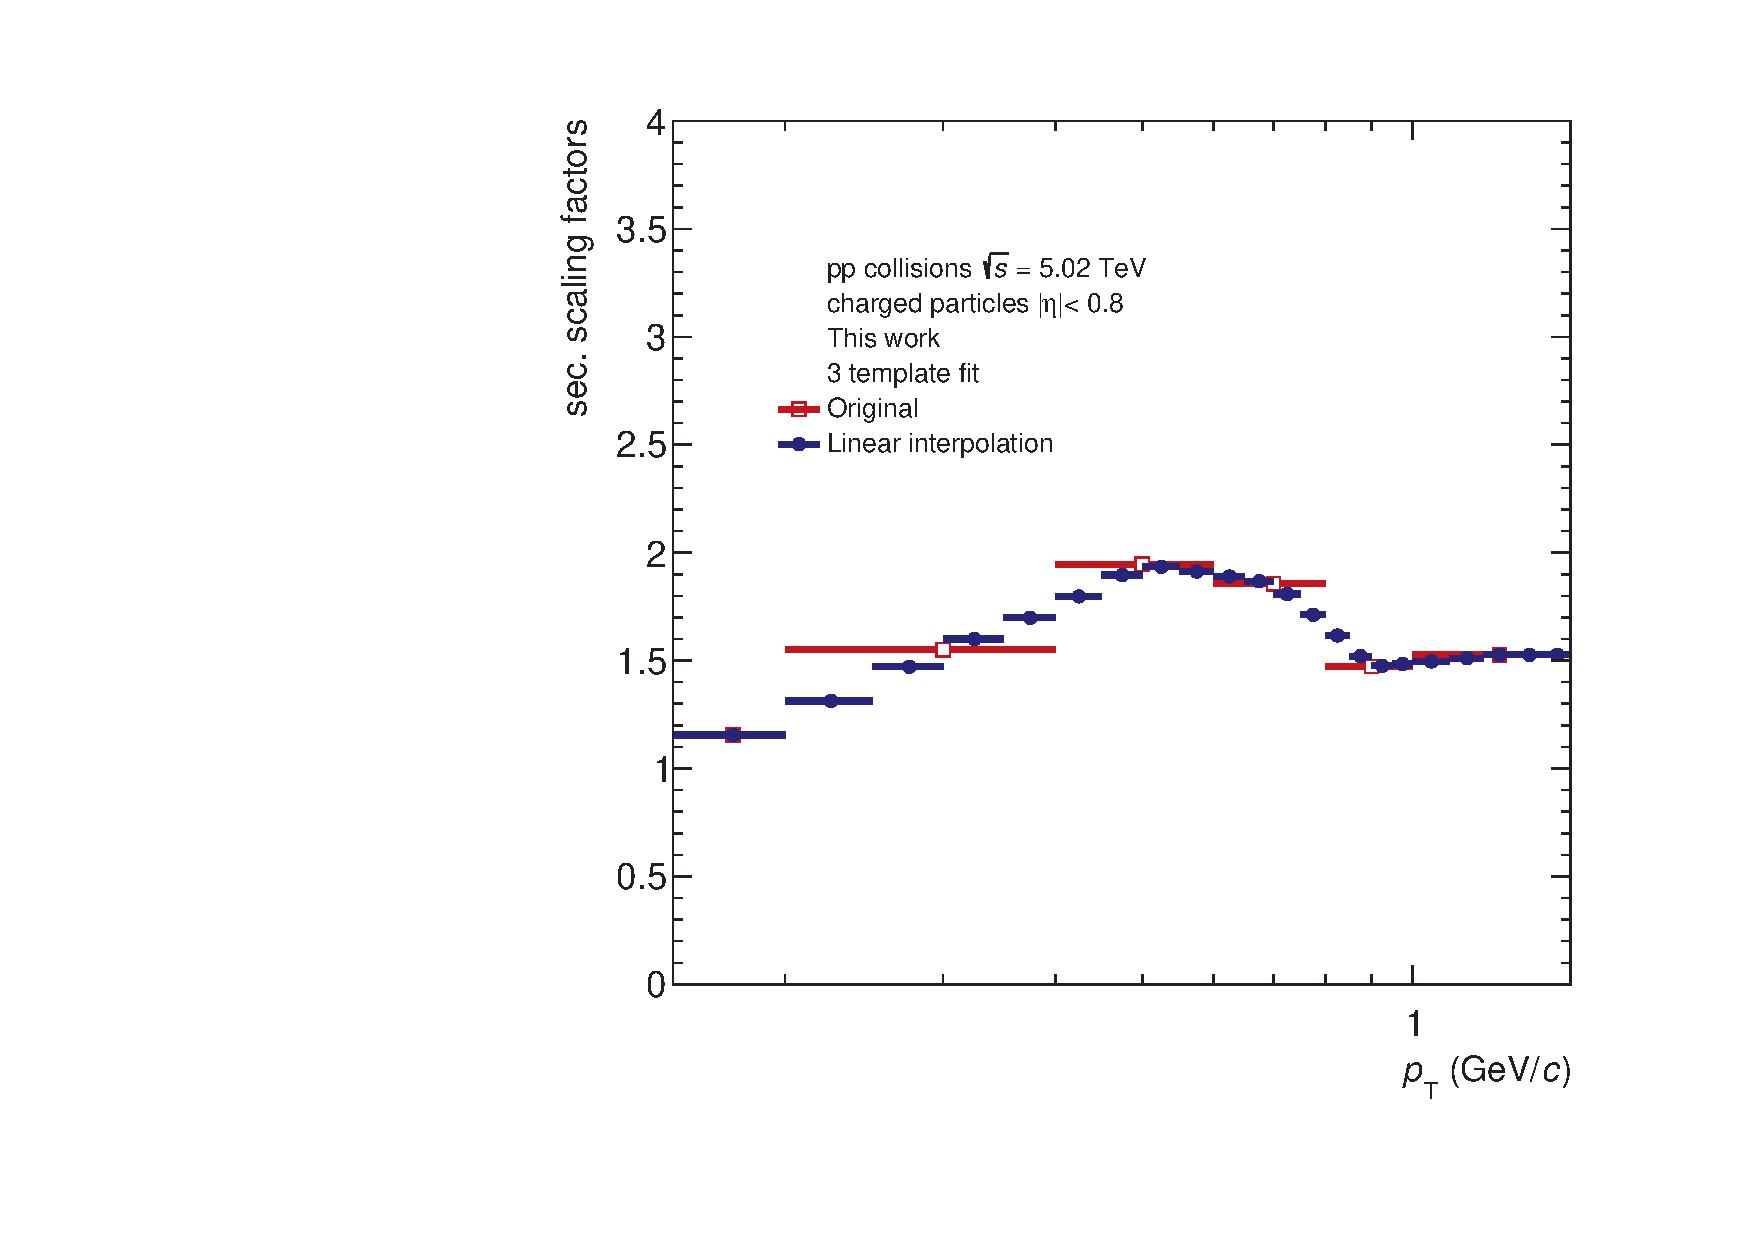
\includegraphics[width=11cm]{Plots/secscalingfactors.pdf}  
\caption{Scaling factors used in pp collisions for the correction of the secondary contamination before and after a linear interpolation.}
\label{scalefactors} 
\end{figure}
In Figure \ref{scalefactors}, the resulting scaling factors in pp collisions are shown as an example. To be able to scale the secondary contamination in all \pt intervals, the missing scaling factors are constructed by a linear interpolation as shown in this same figure. For \pt $> 1.5$ GeV/$c$, the scale factor of the last considered \pt interval is used since the amount of secondaries barely varies beyond this range. The corrected contamination by secondaries is shown in Figure \ref{SecCont} with full markers.\\
Moreover, the intervals of the DCA$_{\text{xy}}$ distributions as well as the \pt intervals for which the fit is performed are adjusted by optimizing the deviation of the data points from the fit as function of the DCA$_{\text{xy}}$ as shown in Figure \ref{Pulls}. Here, it can be seen that the template prediction is in good agreement with the the data points in the tails, the region of interest in this approach.\\
To ensure the goodness of the fit, a Pearson's chi-squared test was performed with a significance level of $0.05$ (cite Karl Pearson paper). In this approach, the test statistic ratio $\chi^2$ is computed as follows:
\begin{equation}
\chi^2 = \sum_{\text{i}} \dfrac{(\text{DCA}_\text{data,i} - \text{DCA}_\text{fit,i})^2}{\text{DCA}_\text{fit,i}}
\end{equation}
Following this, the critical $\chi^2$ value is calculated by means of the chi-squared probability distribution function determined by the the number of degrees of freedom in the fit and the significance level. According to the chi-squared test, the evaluated fit is rejected whenever the test statistic $\chi^2$ exceeds the critical $\chi^2$ value. All fits used for the calculation of the scaling factors are statistically significant according to this test. 
\begin{figure}[tb!]
\centering
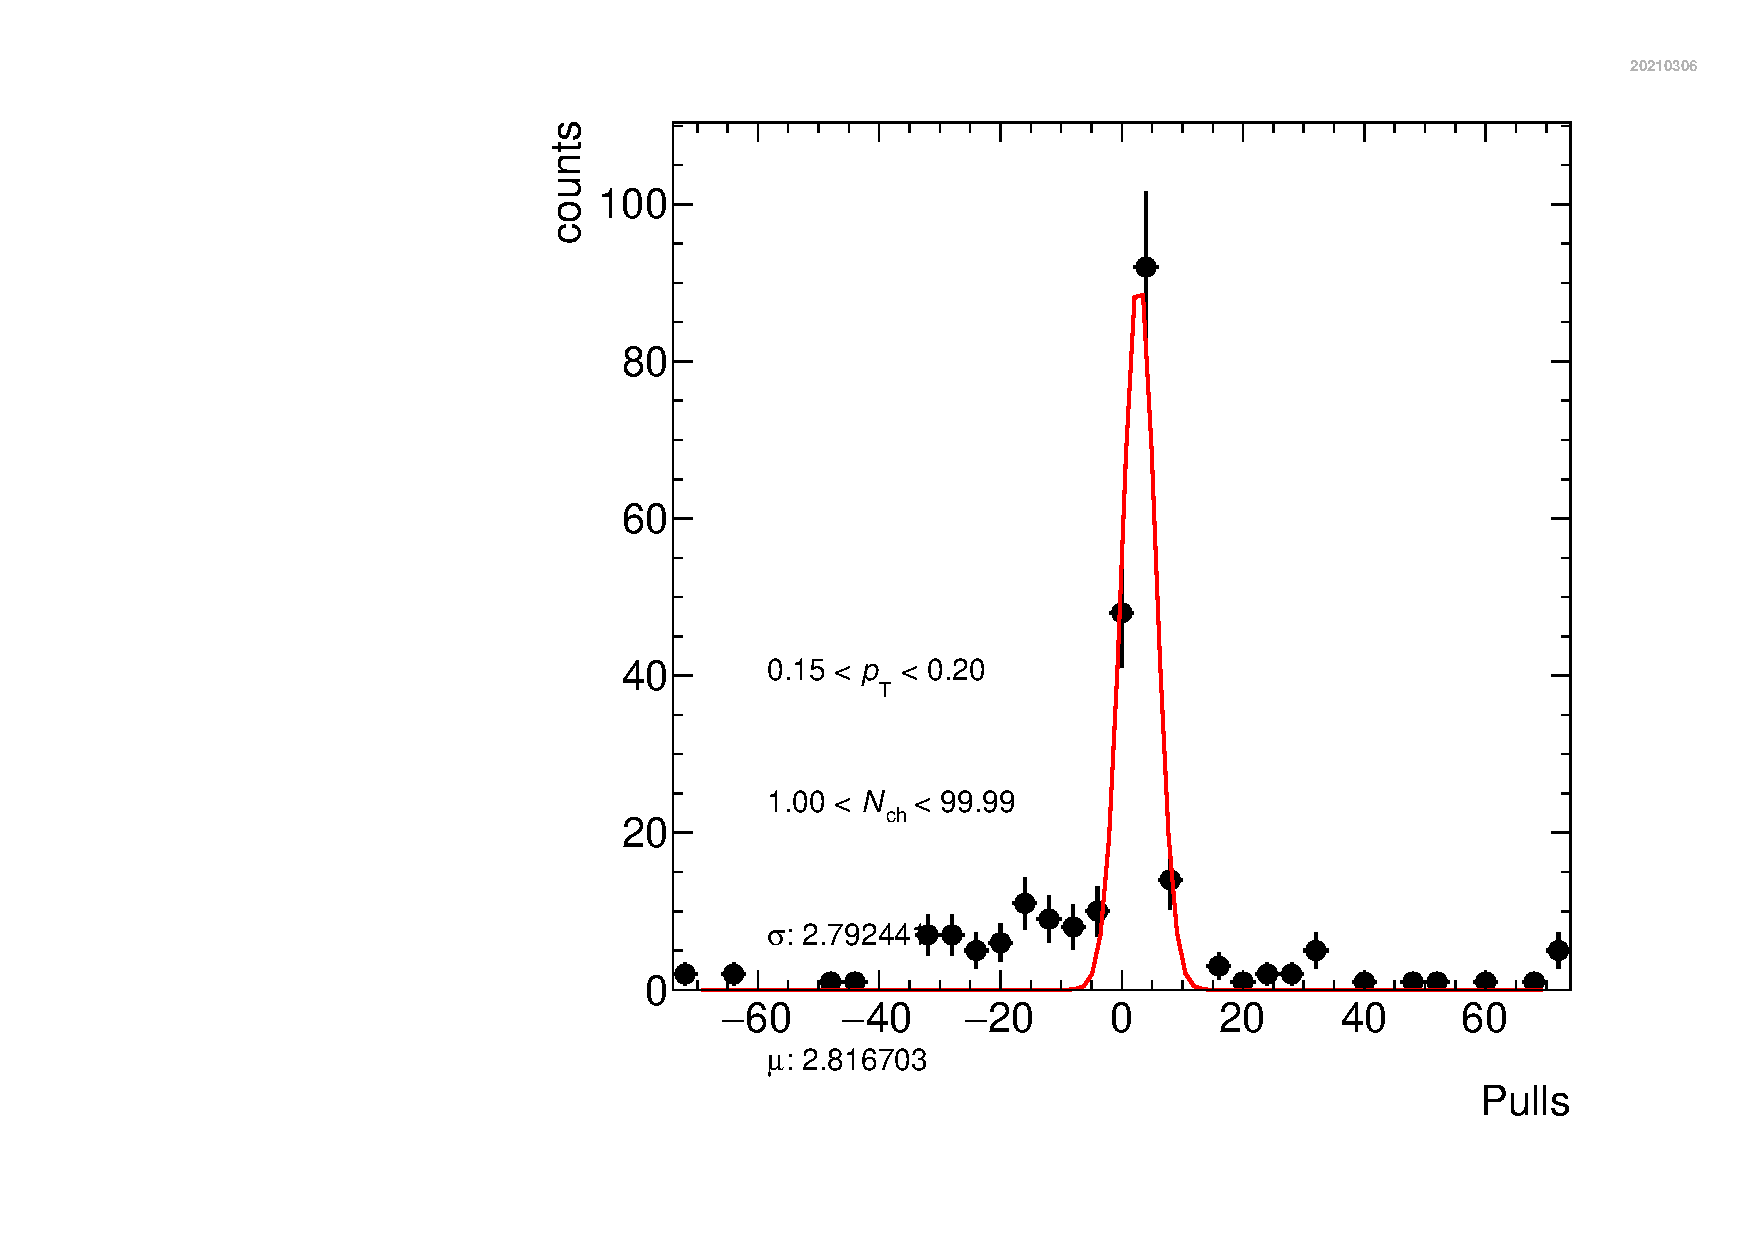
\includegraphics[width=11cm]{Plots/Pulls_Pt0_Mult0.pdf}  
\caption{Deviation of the template prediction from the data points as function of the DCA in pp collisions for the \pt interval $0.15 \leq$ \pt $0.19$ GeV/$c$.}
\label{Pulls}
\end{figure}
\subsection{Transverse momentum resolution}
%cite https://www.physi.uni-heidelberg.de/~fschney/detektoren/detector6.pdf
As discussed in Section (cite section), the trajectory of a charged particle traveling through the TPC is characterized by a helical form caused by the prevailing magnetic field. This phenomenon is conditioned by the Lorentz force which connects the radius $r$ of the track curvature with the transverse momentum \pt of the particle:
\begin{equation}
r = \dfrac{p_\text{T}}{e\cdot B}
\label{radius}
\end{equation}
where $B$ is the magnetic flux density perpendicular to the particle of charge $e$. In practice, the measurement of this radius is demanding since even particles with low transverse momenta present radii that far exceed the outer radius of the TPC. For this reason, the radius is substituted by another quantity which parametrizes the track curvature and which can be measured within the detector volume. This is the so-called sagitta (see Figure \ref{Sagitta}), an arc parameter which turns inverse proportional to the radius of the track for the extreme case of a chord $L<<r$ spanning the base of the arc (cite here):
\begin{equation}
s = \dfrac{l^2}{8r}
\end{equation}
Therefore, we obtain for $B$ given in T, $L$ in m and \pt in GeV/$c$
\begin{equation}
s = \dfrac{0.3e \cdot B \cdot l^2}{8p_\text{T}}
\end{equation}
\begin{figure}[tb!]
\centering
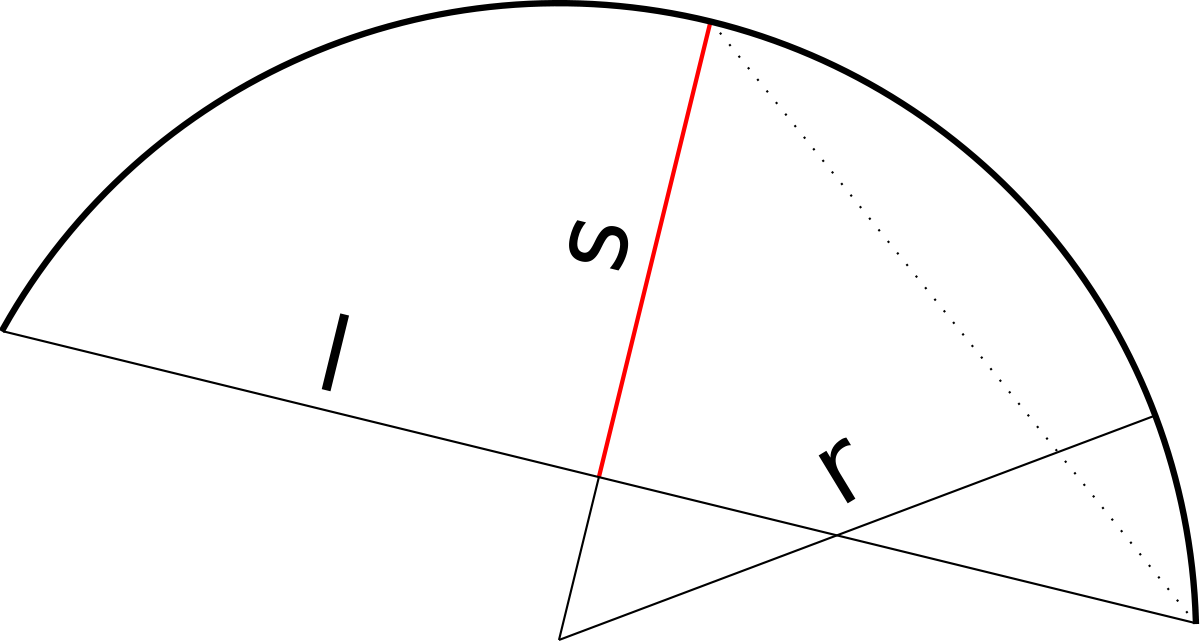
\includegraphics[width=7cm]{Plots/Sagitta.png}  
\caption{Visualization of the radius $r$, the sagitta $s$ and the chord $l$ of a circular arc (cite wikipedia).}
\label{Sagitta}
\end{figure}
\hspace{-0.25cm} The sagitta is measured with an uncertainty due to the spatial resolution of the detectors which in turn implies that the resulting inverse of the transverse momentum is affected by an uncertainty $\sigma(1/p_\text{T})$. It can be then shown that the relative transverse momentum resolution $\sigma(p_\text{T})/p_\text{T}$ can be approximated by (cite knichel):
\begin{equation}
\dfrac{\sigma(p_\text{T})}{p_\text{T}} \approx p_\text{T} \cdot \sigma(1/p_\text{T})
\end{equation}
\begin{figure}[tb!]
\centering
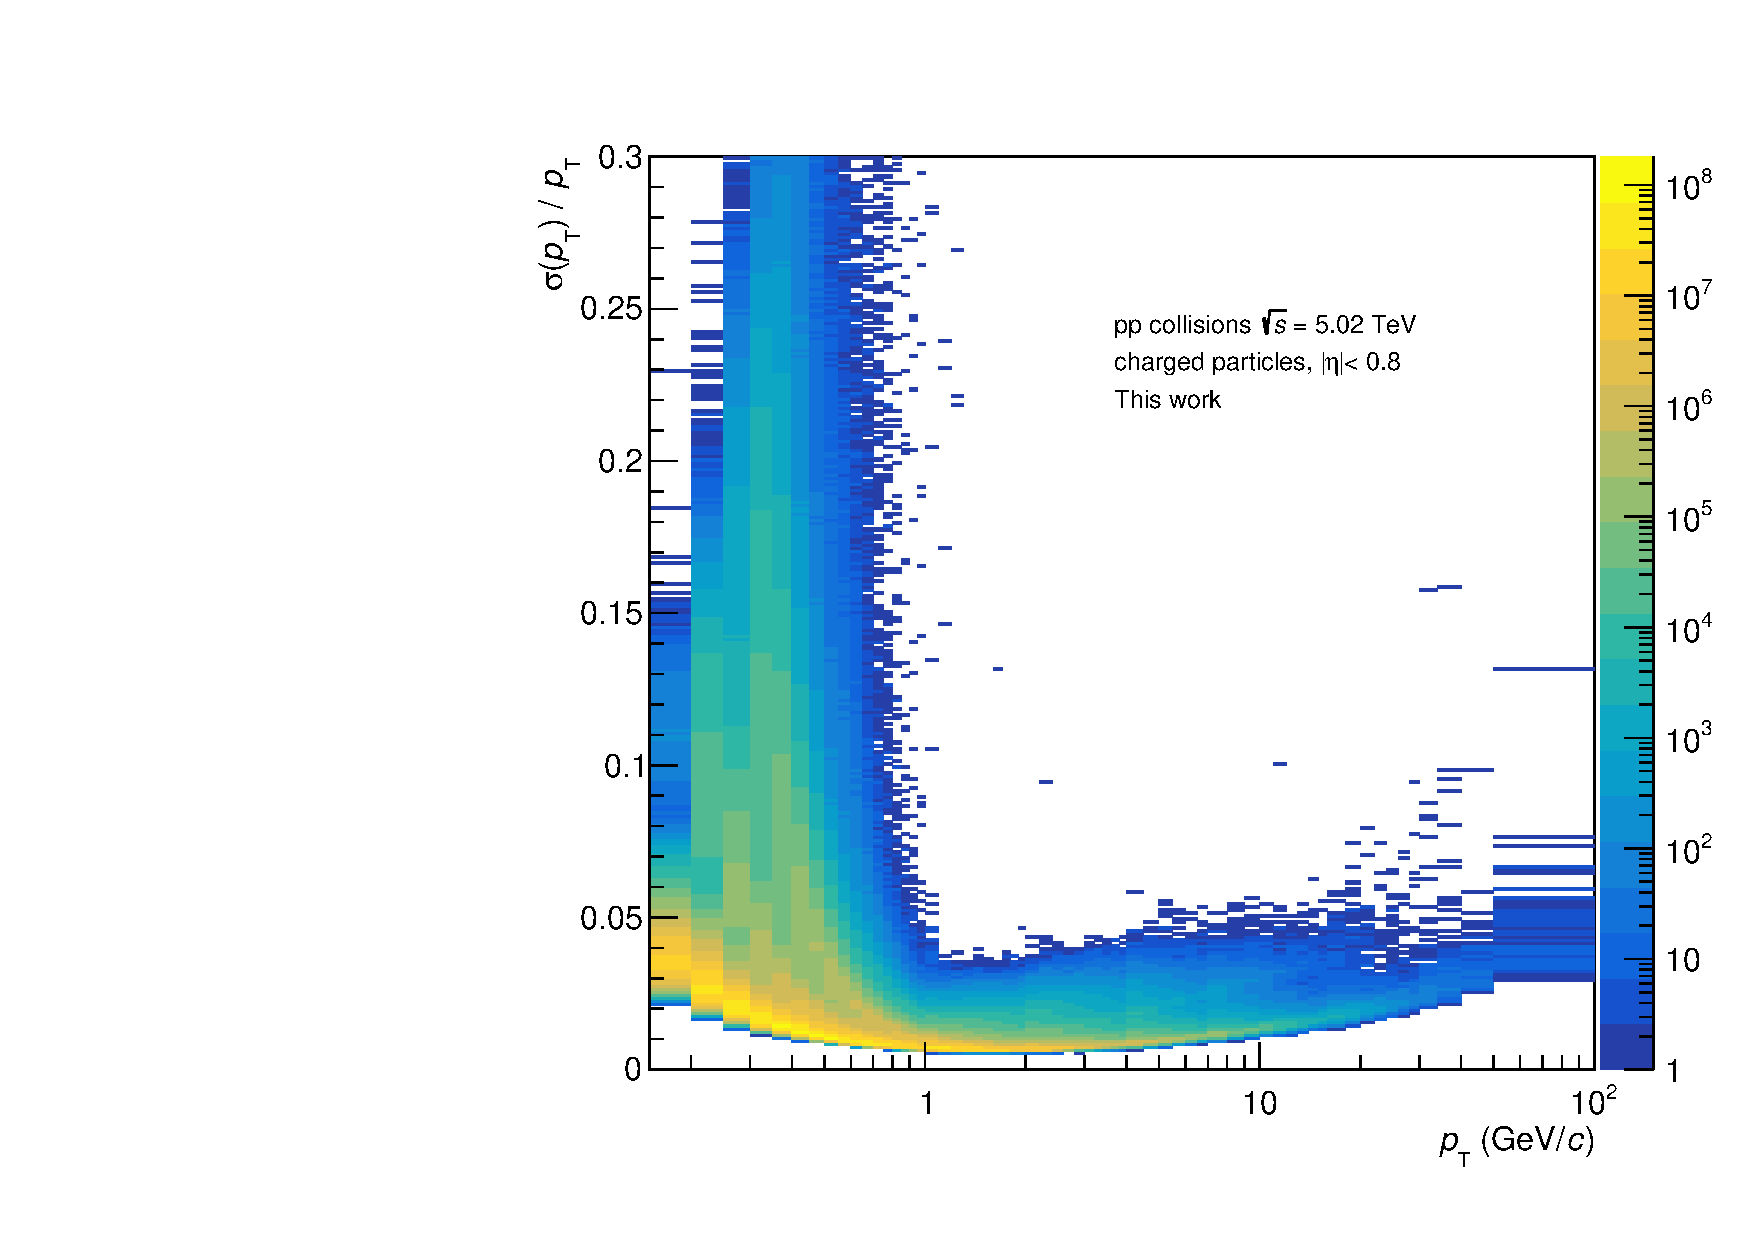
\includegraphics[width=12cm]{Plots/ptReso2D.pdf}  
\caption{Transverse momentum resolution as function of the transverse momentum for pp collisions at $\sqrt{s} = 5.02$ TeV recorded in ALICE in 2017.}
\label{ptReso2D}
\end{figure}
\begin{figure}[tb!]
\centering
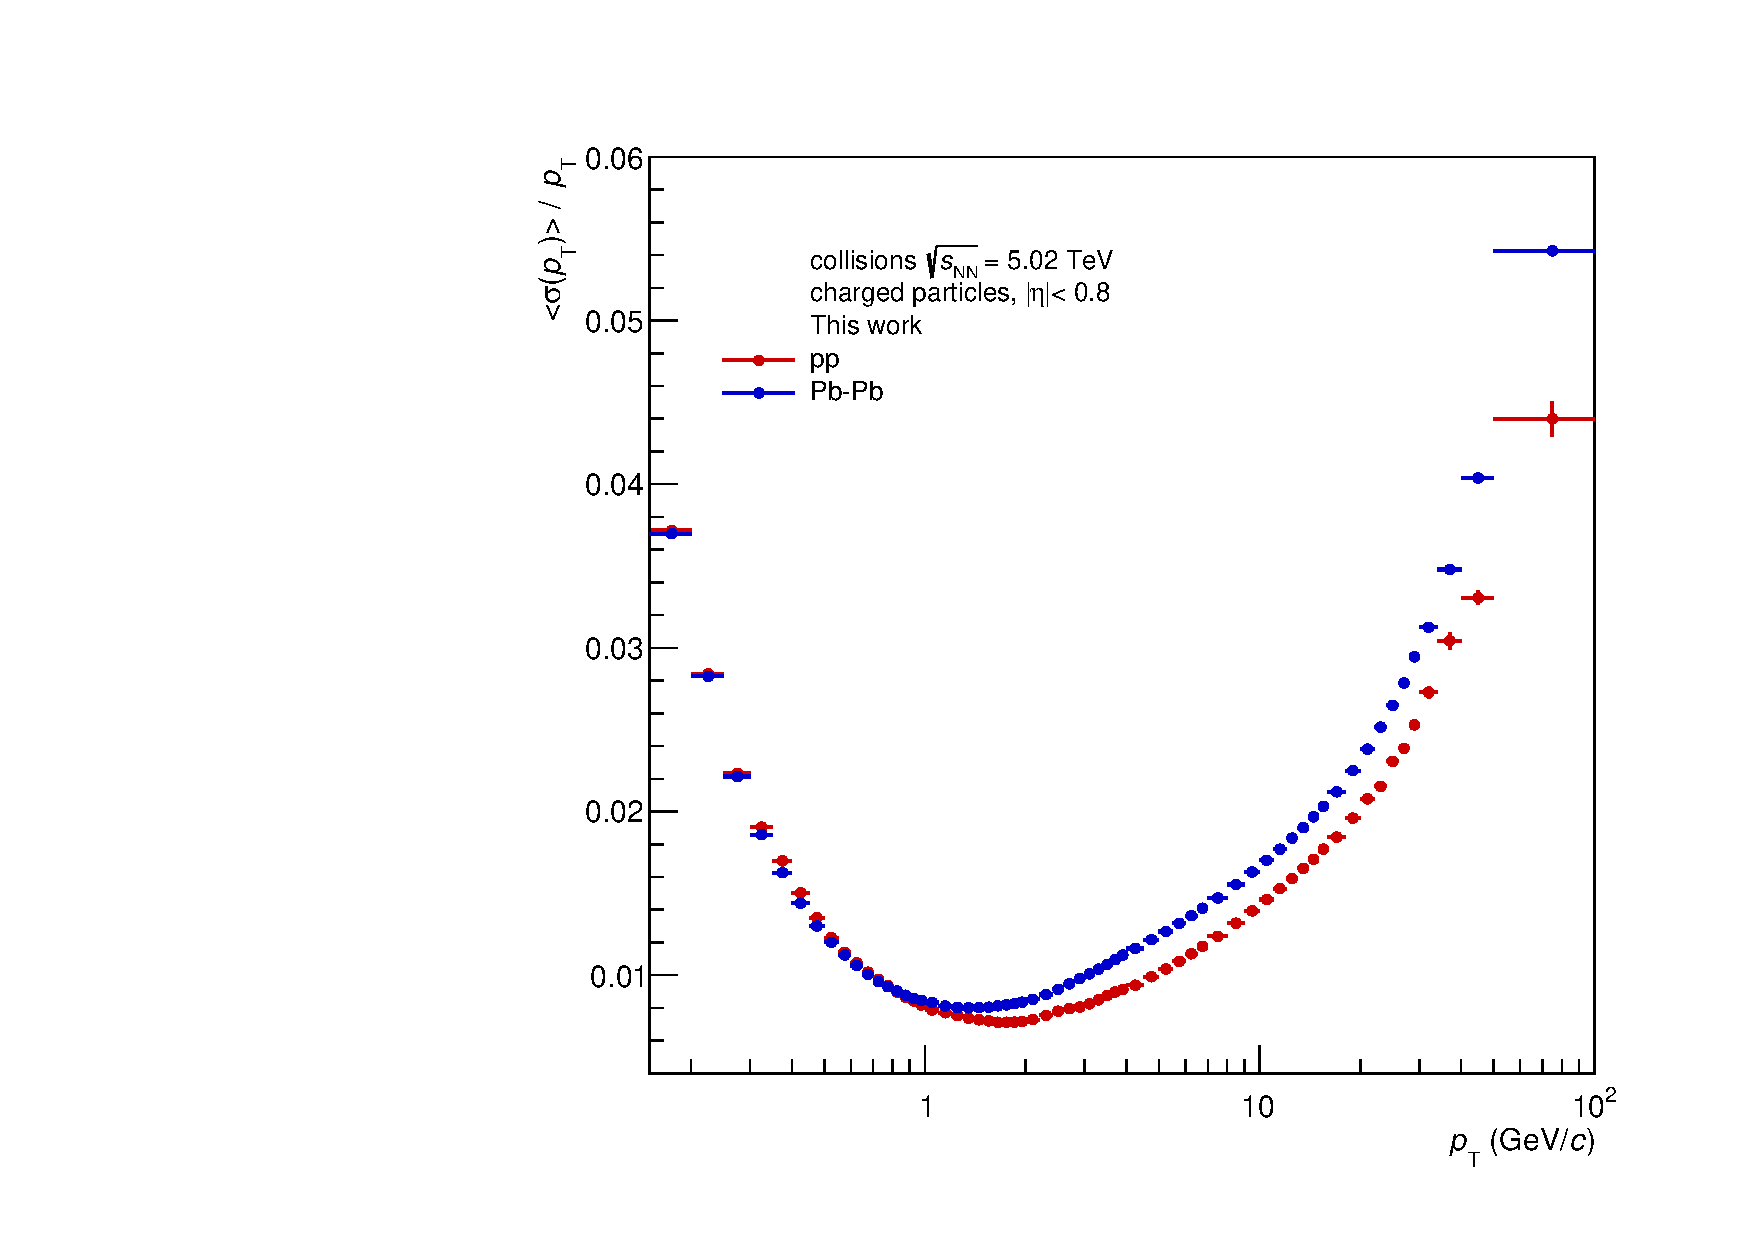
\includegraphics[width=12cm]{Plots/ptReso1D.pdf}  
\caption{The mean relative transverse momentum resolutions are obtained as function of the transverse momentum for pp and MB Pb-Pb collisions.}
\label{ptReso1D}
\end{figure}
\hspace{-0.3cm} In Figure \ref{ptReso2D}, the distribution of $\sigma(p_\text{T})/p_\text{T}$ is shown as function of \pt for the analysed pp collisions. The three visible structures at low \pt can be explained by the interaction of charged particles with the detector material of the ITS. When a particle crosses the detector, it undergoes multiple scattering and its trajectory is consequently deflected by small angles affecting thereby the track parameters determination. Such an effect is dependent on the particle mass and the observed distinct trends of the resolution correspond, in decreasing order of uncertainty, to protons, kaons and pions. For a more clear representation, the mean value $\langle\sigma(p_\text{T})/p_\text{T}\rangle$ is calculated in each \pt interval of this distribution as well as for its analogous in MB Pb-Pb collisions. As result, the mean relative \pt resolution as function of $p_\text{T}$ is obtained as shown in Figure \ref{ptReso1D}. At low $p_\text{T}$, the relative $p_\text{T}$-resolutions are influenced mainly by the multiple scattering of the charged particles in the detector material. In this region, the results in pp and Pb-Pb as well as among the different centrality classes resemble each other. At $p_\text{T} = 0.15$ GeV/$c$, the resolution is on average around 3.7\%.\\
The effect of the multiple scattering dissipates gradually until the distribution hits the minimum around 1.5 GeV/$c$ with a \pt resolution of approximately 0.7\% in pp and 0.8\% in Pb-Pb. At high $p_\text{T}$, charged particles experience a less pronounced curvature according to Equation \ref{radius}, which causes a deterioration of the spatial resolution. As consequence, the uncertainty grows linearly reaching values of 4.4\% in pp and 5.4\% in Pb-Pb.\\
Since the measurement of \pt is smeared due to the resolution, the \pt spectra must be accordingly corrected. While the smearing has a minor effect on the \pt spectra at low \pt given the smooth slope of the distributions, it becomes more pronounced in the high \pt region, where the \pt spectra present a steeply falling shape. The corresponding correction is thus applied in the range $7 \leq p_\text{T} \leq 100$ GeV/$c$ by means of a $p_\text{T}$-dependent factor $c_\text{res}$ calculated as follows: 
\begin{equation}
c_\text{res}(p_\text{T}) = \dfrac{(\text{d}N/\text{d}p_\text{T})_\text{smeared}}{(\text{d}N/\text{d}p_\text{T})_\text{true}}
\end{equation}
where the numerator corresponds to the measured \pt distribution, while the denominator is a \pt distribution free of smearing. As starting point, the \pt distributions from the previous ALICE publication, depicted in Section (cite theo. section), are used  given that they offer a good approximation of the true \pt distributions. As consequence, correction factors are calculated for pp collisions and for each centrality class in Pb-Pb. For the calculation of $c_\text{res}(p_\text{T})$, these \pt distributions are smeared in such a way as to emulate the effect of the \pt resolution. The details of the used approach are outlined in the following.
\subsubsection{Calculation of the correction factor}
\begin{figure}[tb!]
\centering
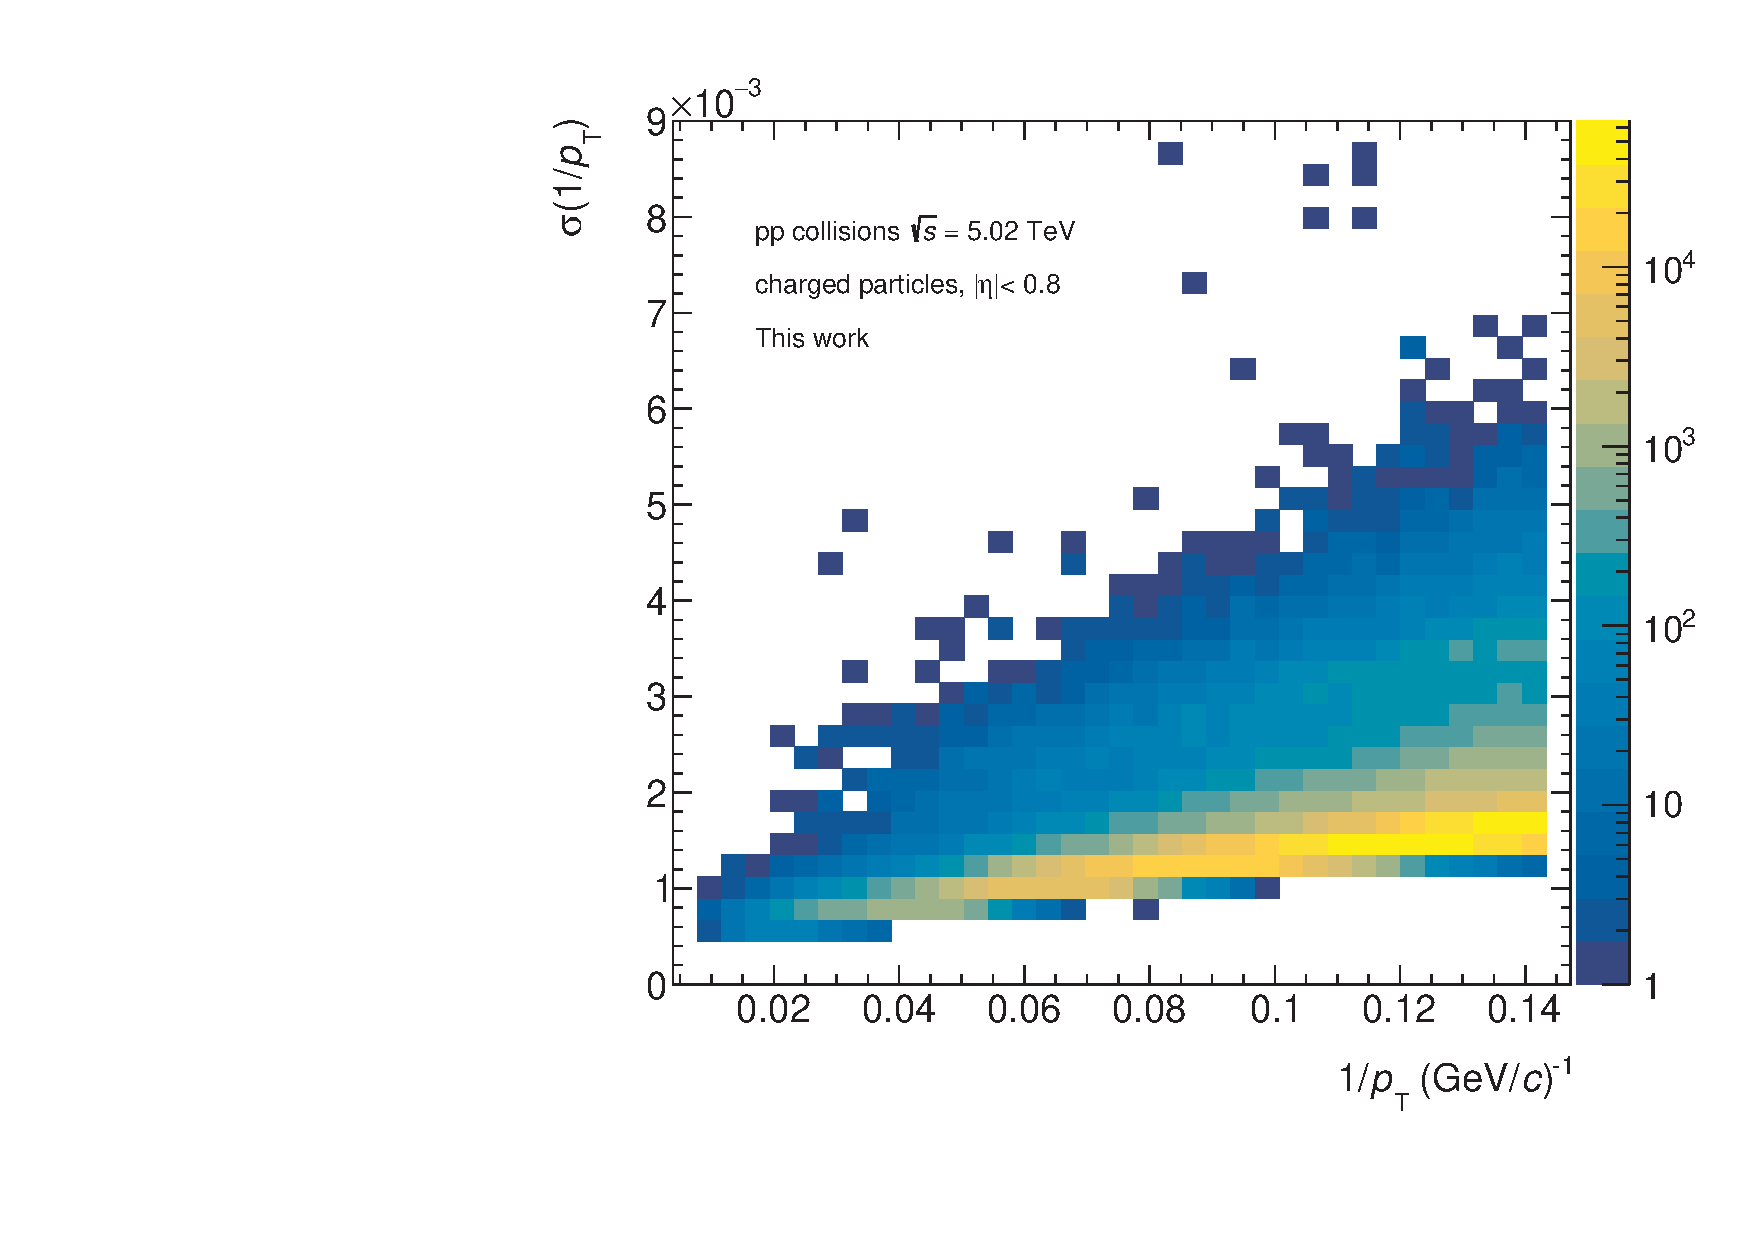
\includegraphics[width=0.495\textwidth]{Plots/reso2dim.pdf}  
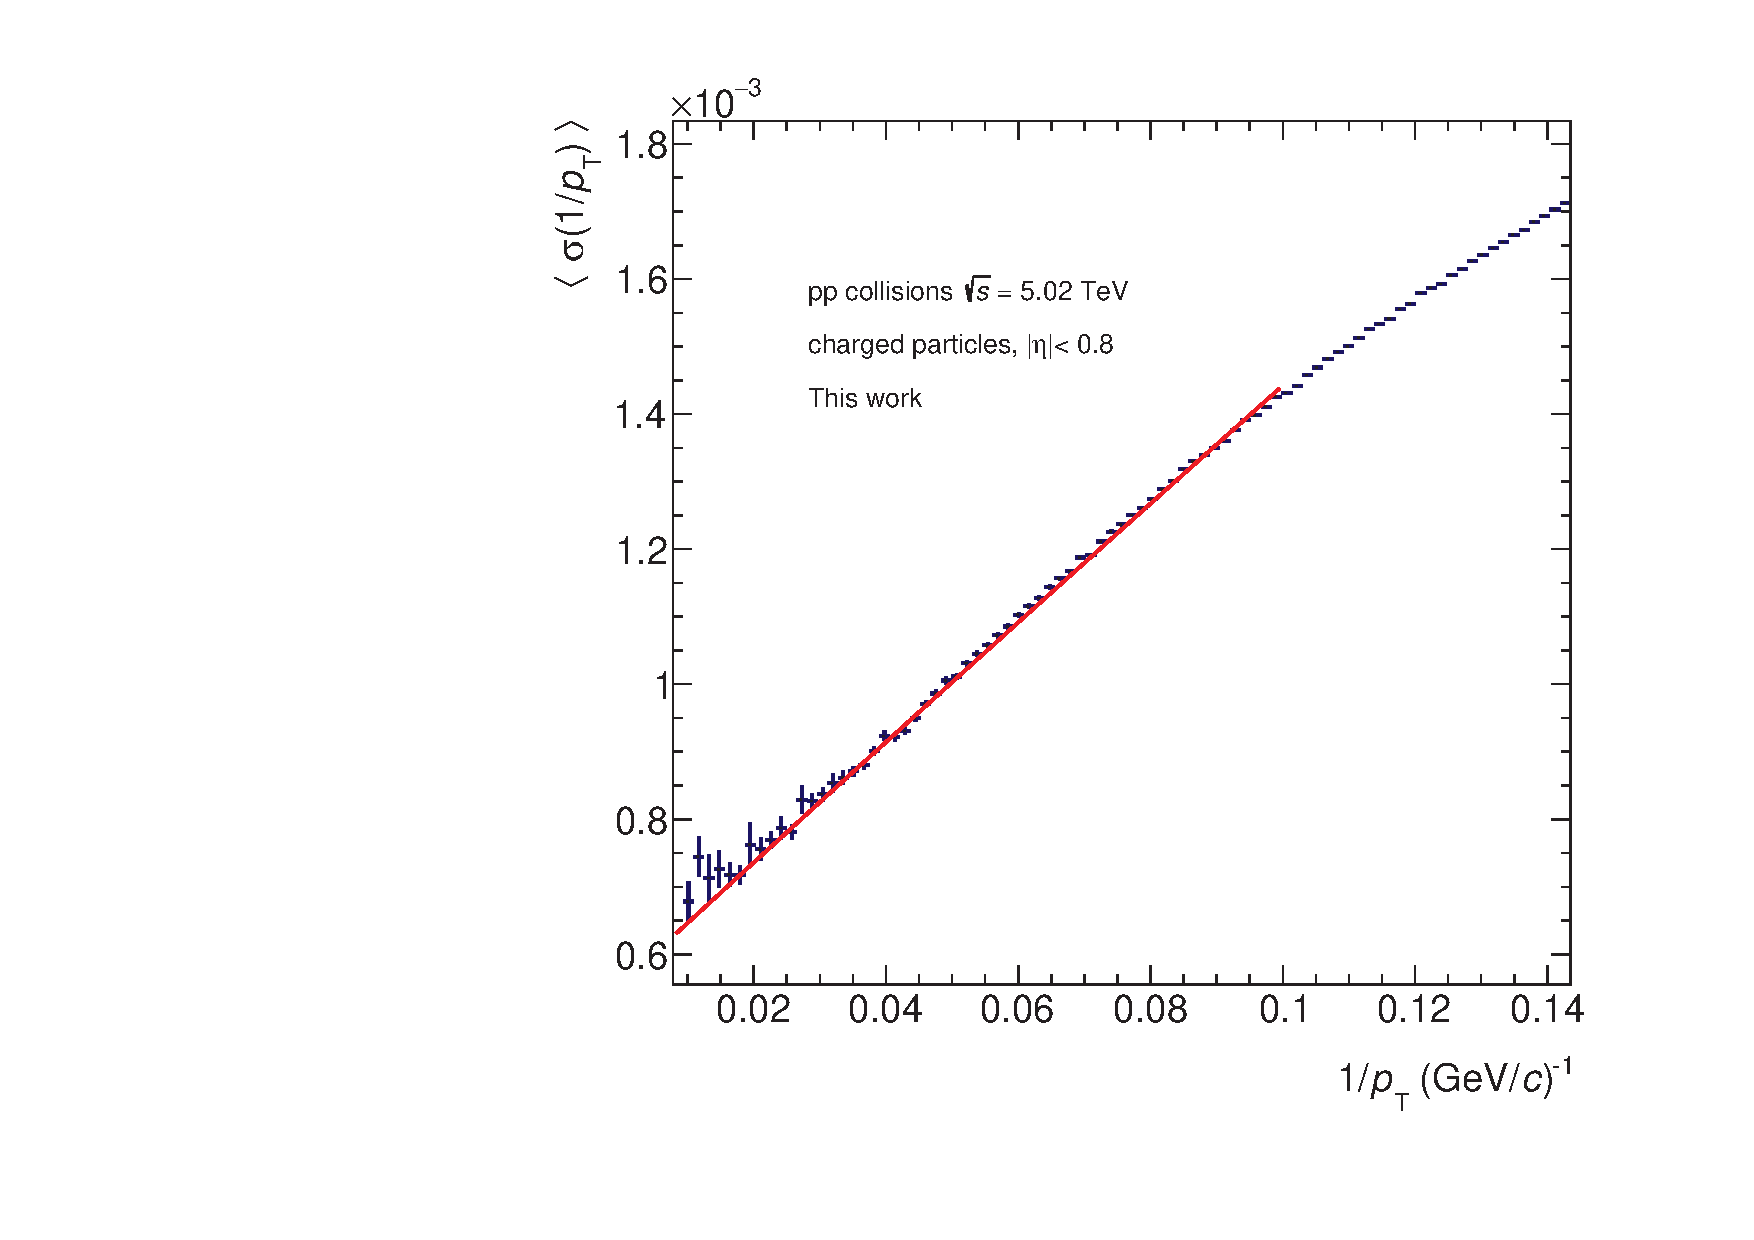
\includegraphics[width=0.495\textwidth]{Plots/fitfunc.pdf}  
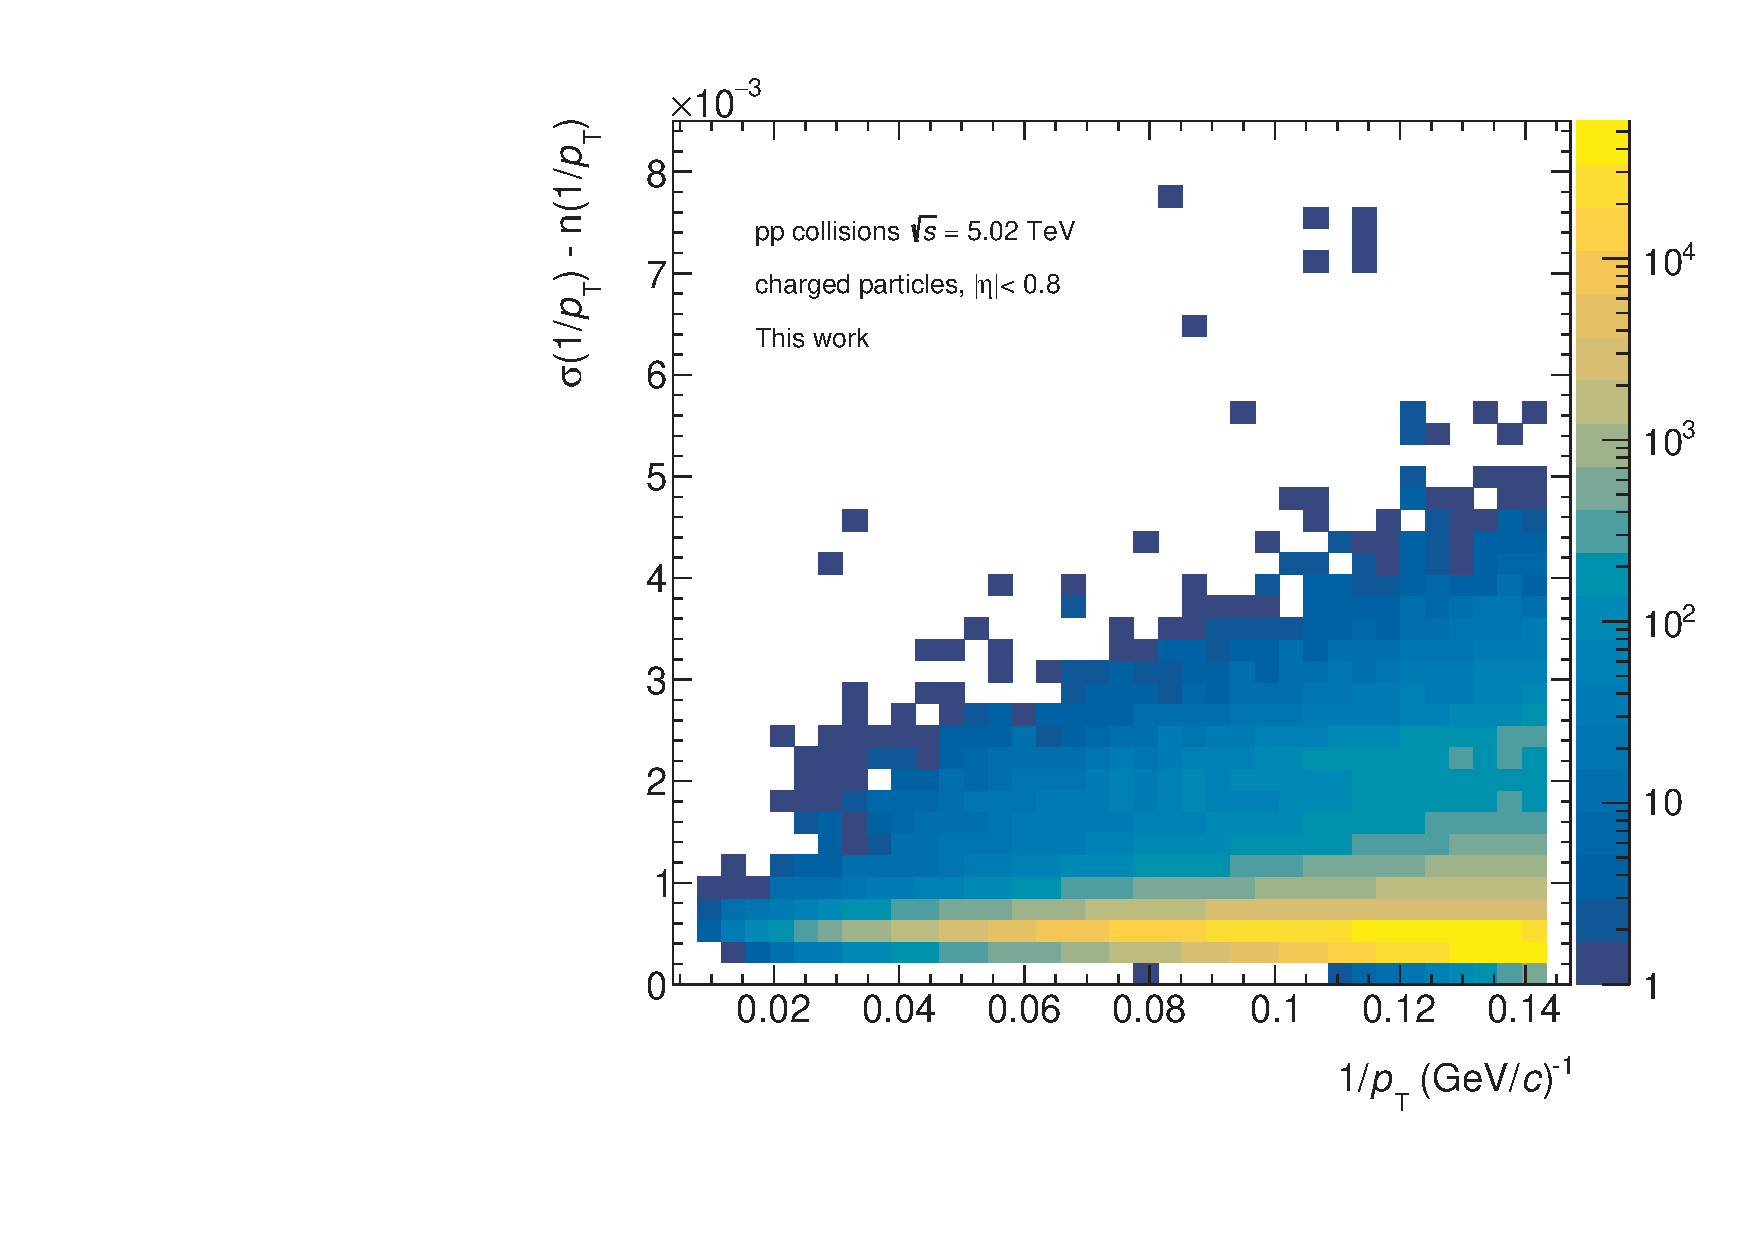
\includegraphics[width=0.495\textwidth]{Plots/scaledcov.pdf}  
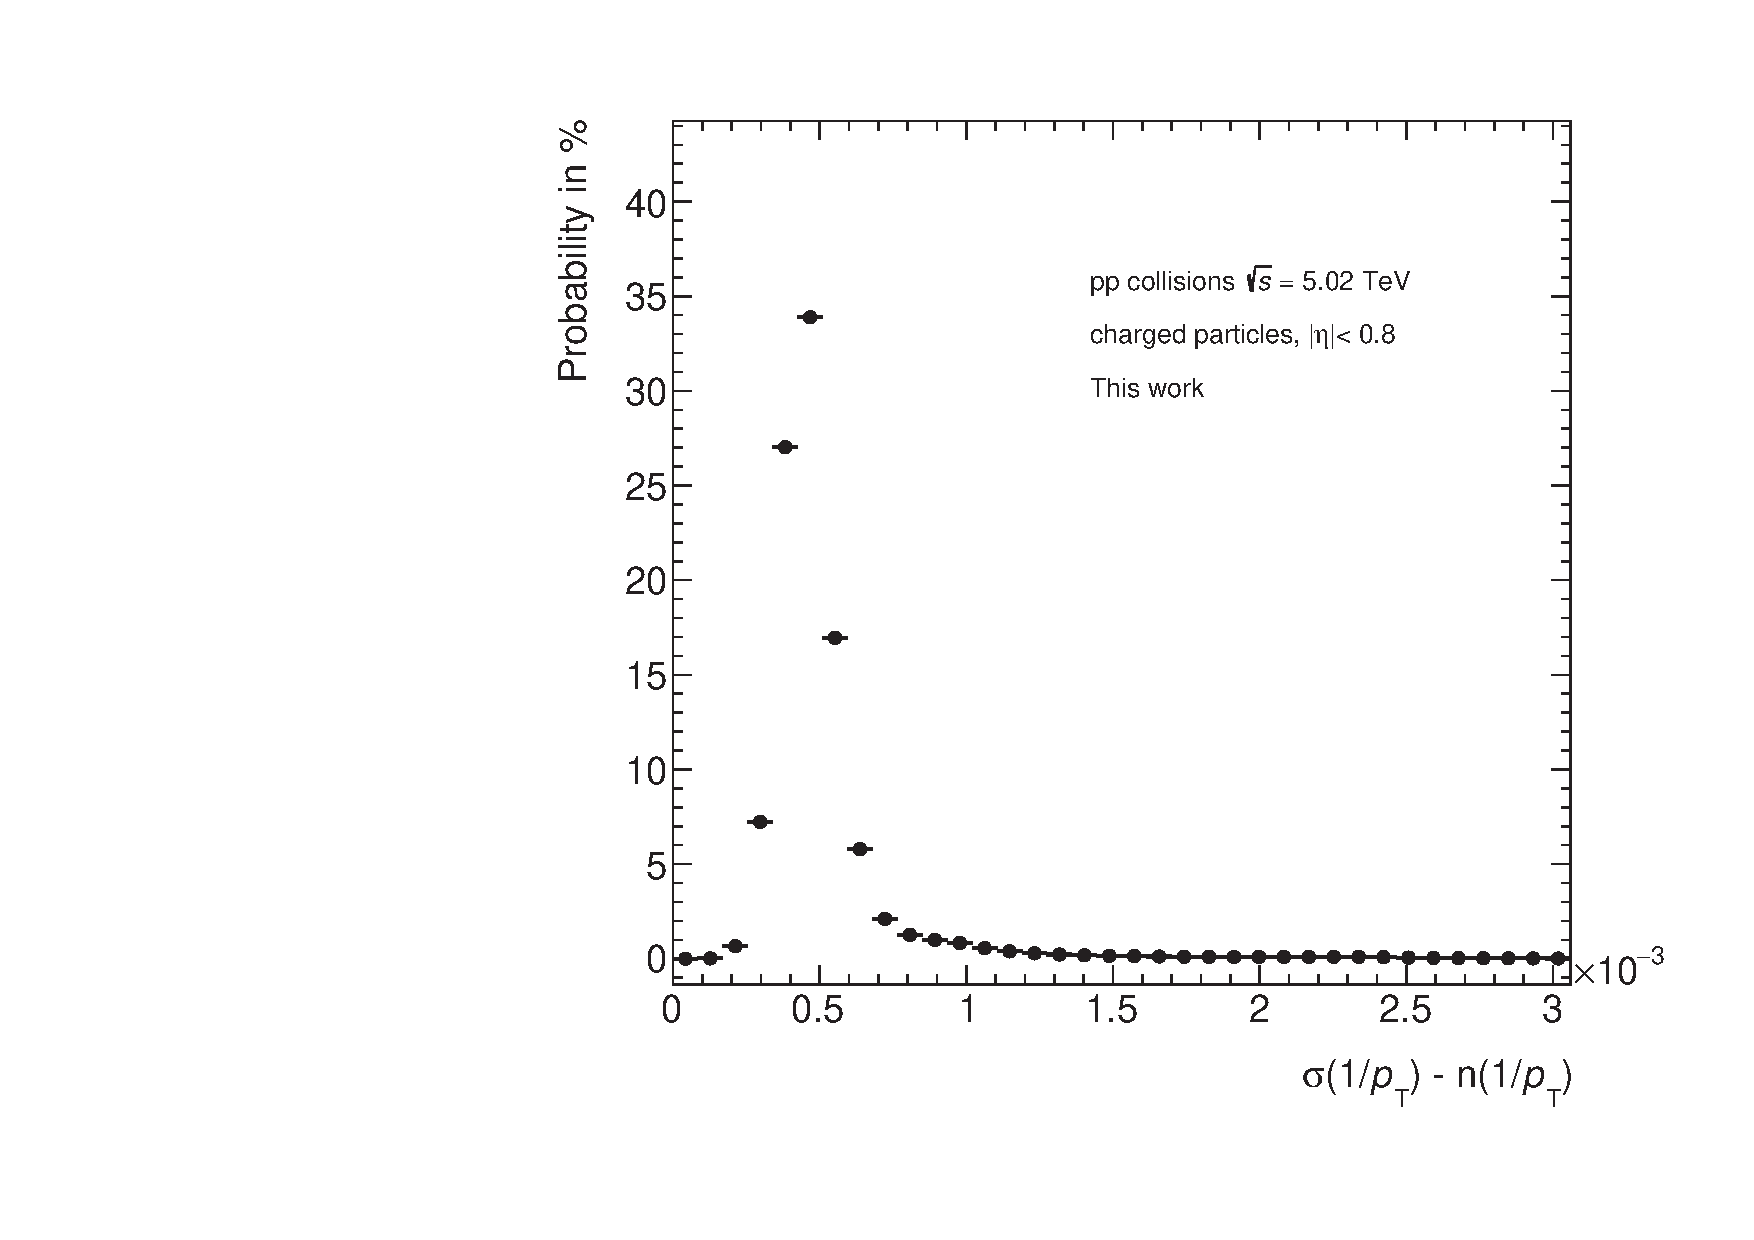
\includegraphics[width=0.495\textwidth]{Plots/probabilitydist.pdf}  
\caption{\textbf{Top.} Left: Two-dimensional distribution of the uncertainty on the inverse of the transverse momentum $\sigma(1/p_{\mathrm{T}})$ as function of $1/p_{\mathrm{T}}$. Right: 2nd order polynomial parametrization $n(1/p_{\mathrm{T}})$ of the mean uncertainty $\langle\sigma(1/p_\text{T})\rangle$ as function of $1/p_{\mathrm{T}}$. \textbf{Bottom.} Left: Two-dimensional distribution of the scaled uncertainty $\sigma(1/p_{\mathrm{T}})$ as function of $1/p_{\mathrm{T}}$. Right: Probability function of $\sigma(1/p_\text{T})$ obtained after projecting the scaled uncertainty into the $y$-axis.}
\label{4plots}
\end{figure}
\begin{figure}[tb!]
\centering
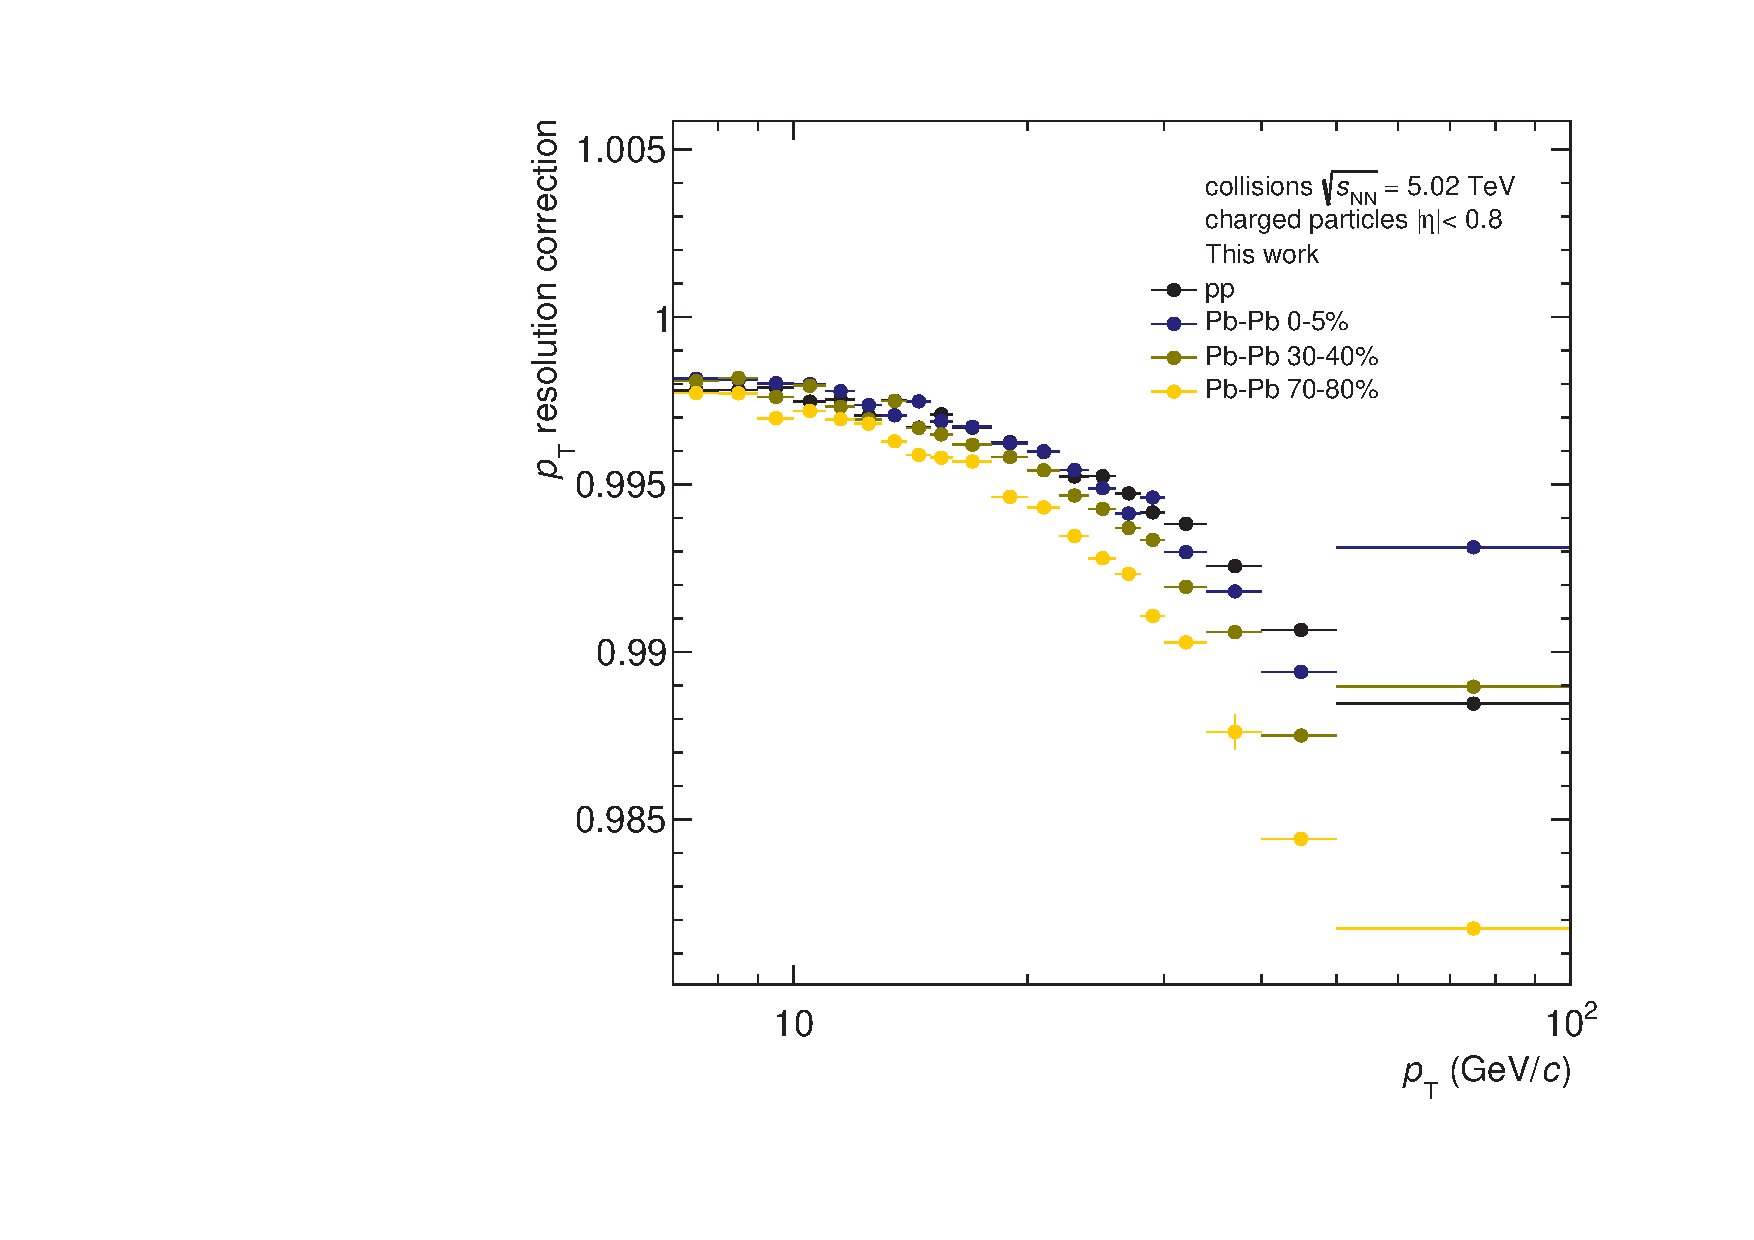
\includegraphics[width=12cm]{Plots/ptrescorrppPbPb.pdf}  
\caption{\pt resolution correction factor as function of $p_{\mathrm{T}}$ in pp and in three centrality classes of Pb-Pb collisions at $\sqrt{s} = 5.02$ TeV recorded in ALICE in 2017.}
\label{ptrescorrppPbPb}
\end{figure}
The smearing is carried out through a simulation that uses as input a sample of filtered high \pt tracks that underwent the same track requirements summarized in Table \ref{tab:Cuts}. The parameter $\sigma(1/p_\text{T})$ of these tracks is considered as function of $1/p_\text{T}$ as shown in the top-left panel of Figure \ref{4plots} for the case of pp collisions. This two-dimensional representation is converted to a distribution of the mean uncertainty $\langle\sigma(1/p_\text{T})\rangle$ as function of $1/p_\text{T}$. In addition, this distribution is parametrized with a 2nd order polynomial $n(1/p_\text{T})$ which is then subtracted from the original uncertainty $\sigma(1/p_\text{T})$ in order to reduce statistical fluctuations as seen in the top-right panel of Figure \ref{4plots}. The scaled $\sigma(1/p_\text{T})$ distribution (see bottom left panel of Figure \ref{4plots}) is subsequently projected into the $y$-axis obtaining thereby a distribution that reveals the probability function of $\sigma(1/p_\text{T})$ as shown in the bottom-right panel of Figure \ref{4plots}.\\
After determining the shape of $\sigma(1/p_\text{T})$, the smearing is performed. In this process, tracks are simulated and distributed according to a power-law fit of the true \pt distributions in the range $7 \leq p_\text{T} \leq 100$ GeV/$c$. These are then transformed in $1/p_\text{T}$ distributions. Moreover, each $1/p_\text{T}$ value is smeared according to a Gaussian with a standard deviation generated randomly in respect of the probability function of $\sigma(1/p_\text{T})$. This standard deviation is first adjusted with an additive factor extracted from an evaluation of the polynomial $n(1/p_\text{T})$ as re-correction for the above mentioned suppression of statistical fluctuations (see bottom-left panel of Figure \ref{4plots} ). Finally, the smeared $1/p_\text{T}$ distribution is re-converted in a \pt spectrum.\\
The \pt resolution correction factors are calculated by means of the quotient of the original simulated \pt spectrum and the smeared one. In Figure \ref{ptrescorrppPbPb}, the resulting correction factors for the analyzed pp and for central, semi-central and peripheral Pb-Pb collisions are respectively illustrated. The correction factor falls monotonically and the effect finds its maximum at the largest \pt interval with a percentage value of around 1.2\% (1\%) for pp (Pb-Pb) collisions. On the other hand, the Pb-Pb results behave similarly as in the pp data collection. Nevertheless, a centrality dependence of the correction factors is observed which originates from the different steepness of the true \pt spectra.
\section{Implementation of the corrections}
\label{secCorr}
The analysis strategies presented in the previous sections aim to mitigate the effects derived from the detector response that distorts the data sample. As already mentioned, the track-level corrections affect the shape of the primary track distribution $N(p_\text{T})$. The corrected primary track distribution $N_\text{corr}(p_\text{T})$ can be defined as follows:
\begin{equation}
\begin{split}
N_\text{corr}(p_\text{T}) = & N_\text{raw}(p_\text{T}) \times \dfrac{1}{\epsilon(p_\text{T}) \cdot c_\text{par comp}(p_\text{T})} \\
& \times (1 - c_\text{cont}(p_\text{T}) \cdot c_\text{sec sca}(p_\text{T})) \\
&\times \dfrac{1}{c_\text{reso}(p_\text{T})} \times \dfrac{1}{\chi_\text{sig loss}(p_\text{T})} 
\end{split}
\end{equation}
where $\epsilon(p_\text{T})$ is the tracking efficiency, $c_\text{par comp}(p_\text{T})$ the particle composition correction, $c_\text{cont}(p_\text{T})$ the secondary contamination correction, $c_\text{sec sca}(p_\text{T})$ the secondary scaling, $c_\text{reso}(p_\text{T})$ the \pt resolution correction and $\chi_\text{sig loss}(p_\text{T})$ the signal loss, which is only applied in pp collisions. Once the corrections are implemented, the \pt distributions can be calculated in respect of the definitions discussed in Section (cite theory section).
According to the definition of the nuclear modification factor, the results in pp collisions are expressed in form of a differential cross section: 
\begin{equation}
\label{EqdiffCross}
\dfrac{\text{d}^2 \sigma^\text{pp}_\text{ch} }{\text{d}\eta \text{d}p_\text{T}} = \sigma_\text{vis} \cdot \dfrac{1}{N_\text{INEL}} \cdot \dfrac{\text{d}^2 N^\text{pp}	_\text{corr}}{\text{d}\eta \text{d}p_\text{T}}
\end{equation}
where $N_\text{INEL}$ corresponds to the total number of inelastic events and $\sigma_\text{vis}$ the visible inelastic cross section as already explained in Section \ref{Norm}. 
In the case of Pb-Pb collisions, the physical quantity used for the determination of nuclear modification factors is the invariant yield and it is calculated as follows
\begin{equation}
\label{Eqinyield}
\dfrac{\text{d}^2 N^\text{Pb-Pb}_\text{ch}}{\text{d}\eta \text{d}p_\text{T}} = \dfrac{1}{N_\text{INEL}} \cdot \dfrac{\text{d}^2 N^\text{Pb-Pb}_\text{corr}}{\text{d}\eta \text{d}p_\text{T}}
\end{equation}
\section{Systematic uncertainties}
MC simulations aim to reproduce accurately the detector performance so that their information can be used to correct the data. However, the simulations are subject to uncertainties which affect the MC based corrections and therefore the \pt distributions as well as the nuclear modification factors. These are the so-called systematic uncertainties. In this thesis, the source of systematics considered arises from the track selection criteria. However, other sources of systematic uncertainties have been identified in previous measurements of nuclear modification factors (cite paper). In this chapter, these other sources will be described and its impact on the \pt distributions presented.
\subsection{Track selection} 
\label{systracksel}
As explained in Section \ref{TrackSelection}, the track selection has been developed in the course of years and validated through cross-checks. Nevertheless, the choice of the selection criteria, yet justified via these studies, is subjected to a systematic uncertainty. For the calculation of the contributions to the systematic uncertainties, it is assumed that each criterion contributes independently of the rest. For this reason, the total value of $\sigma^\text{sys}_\text{tot}$ is calculated via the root sum squared method:
\begin{equation}
\sigma^\text{sys}_\text{sel,tot} = \sqrt{\left(\sum_{\text{i}}\sigma^\text{sys}_\text{sel,i} \right)^2}
\end{equation} 
To determine the individual contributions, each nominal track requirement listed in Table \ref{tab:Cuts} is varied twice within a range in which it is believed to be physically meaningful. The variations, listed in Table \ref{tab:curVar}, correspond to the maximum and the minimum of this range. Next, the fully corrected \pt distributions are recalculated with each variation. These \pt distributions are compared to the nominal one by means of a ratio, obtaining as result two ratios for each track cut, with the exception of the required hit in the SPD. Finally, the two ratios are evaluated in each \pt interval and the largest deviation from the nominal \pt spectrum between the both of them is assumed as systematic uncertainty in the corresponding \pt interval. The resulting systematic uncertainties corresponding to each track cut can be then presented as function of the transverse momentum. The total systematic uncertainty is calculated subsequently applying a root sum squared in each \pt interval among the individual systematic uncertainties. In Figure \ref{SysUncSpec}, the individual and the combined contributions to the systematic uncertainty are given for pp as well as for central, semi-central and peripheral Pb-Pb collisions. \\
In the previous ALICE measurement of nuclear modification factors, the corresponding systematic uncertainties were calculated by propagating the systematic uncertainties on the \pt distributions in pp and Pb-Pb collisions. With the aim of obtaining a more accurate estimation of the systematic uncertainties on $R_\text{Pb-Pb}$, the same approach explained above is used. In Figure \ref{SysUncRaa}, the resulting contributions are shown for pp as well as for central, semi-central and peripheral Pb-Pb collisions.
\begin{table}[tb!]
\renewcommand{\arraystretch}{1.5}
%\rowcolor{bodyBlue}
\centering
\begin{tabular}{l c c c}
\toprule
\rowcolor{headerBlue}  \textbf{Track parameter} &  \textbf{Condition}  &  \multicolumn{2}{c}{\textbf{Variations}} \\
\midrule
\multicolumn{4}{c}{\textbf{Selection of primaries}} \\
\midrule
$\text{DCA}_{z}$ & $\leq 2 $ cm & $1$ cm & $5$ cm\\
$\text{DCA}_{xy}$ & $\leq 7\sigma$ & $4\sigma$ & $10\sigma$ \\
\midrule
\multicolumn{4}{c}{\textbf{ITS selection}} \\
\midrule
at least one hit in the SPD & required  & \multicolumn{2}{c}{not required}\\
$\chi^2$ per ITS cluster  & $\leq 36$ & $\leq 25$ & $\leq 49$ \\
\midrule
\multicolumn{4}{c}{\textbf{TPC selection}} \\
\midrule
$\chi^2$ per TPC cluster (pp collisions) & $\leq 4.0$  & $\leq 3.0$ & $\leq 5.0$\\
$\chi^2$ per TPC cluster (Pb-Pb collisions) & $\leq 2.5$ & $\leq 1.7$ & $\leq 3.4$\\
fraction of shared  TPC clusters&  $\leq 0.4$  & $\leq 0.2$ & $\leq 1.0$ \\
ratio of crossed rows over findable clusters  & $\geq 0.8$ & $\geq 0.7$ & $\geq 0.9$\\
geometric length (dead TPC area) & $3$ cm & $2$ cm & $4$ cm \\
geometric length (track length) & $130$ cm & $120$ cm & $140$ cm\\

\midrule
\multicolumn{4}{c}{\textbf{TPC-ITS selection}} \\
\midrule
$\chi^2$ TPC constrained track vs. global track  & $\leq 36$ & $\leq 25$ & $\leq 49$ \\
\bottomrule
\end{tabular}
\caption{Variations for the standard track selection criteria used for the calculation of the systematic uncertainties.}
\label{tab:curVar}
\end{table}
\begin{figure}[H]
\centering
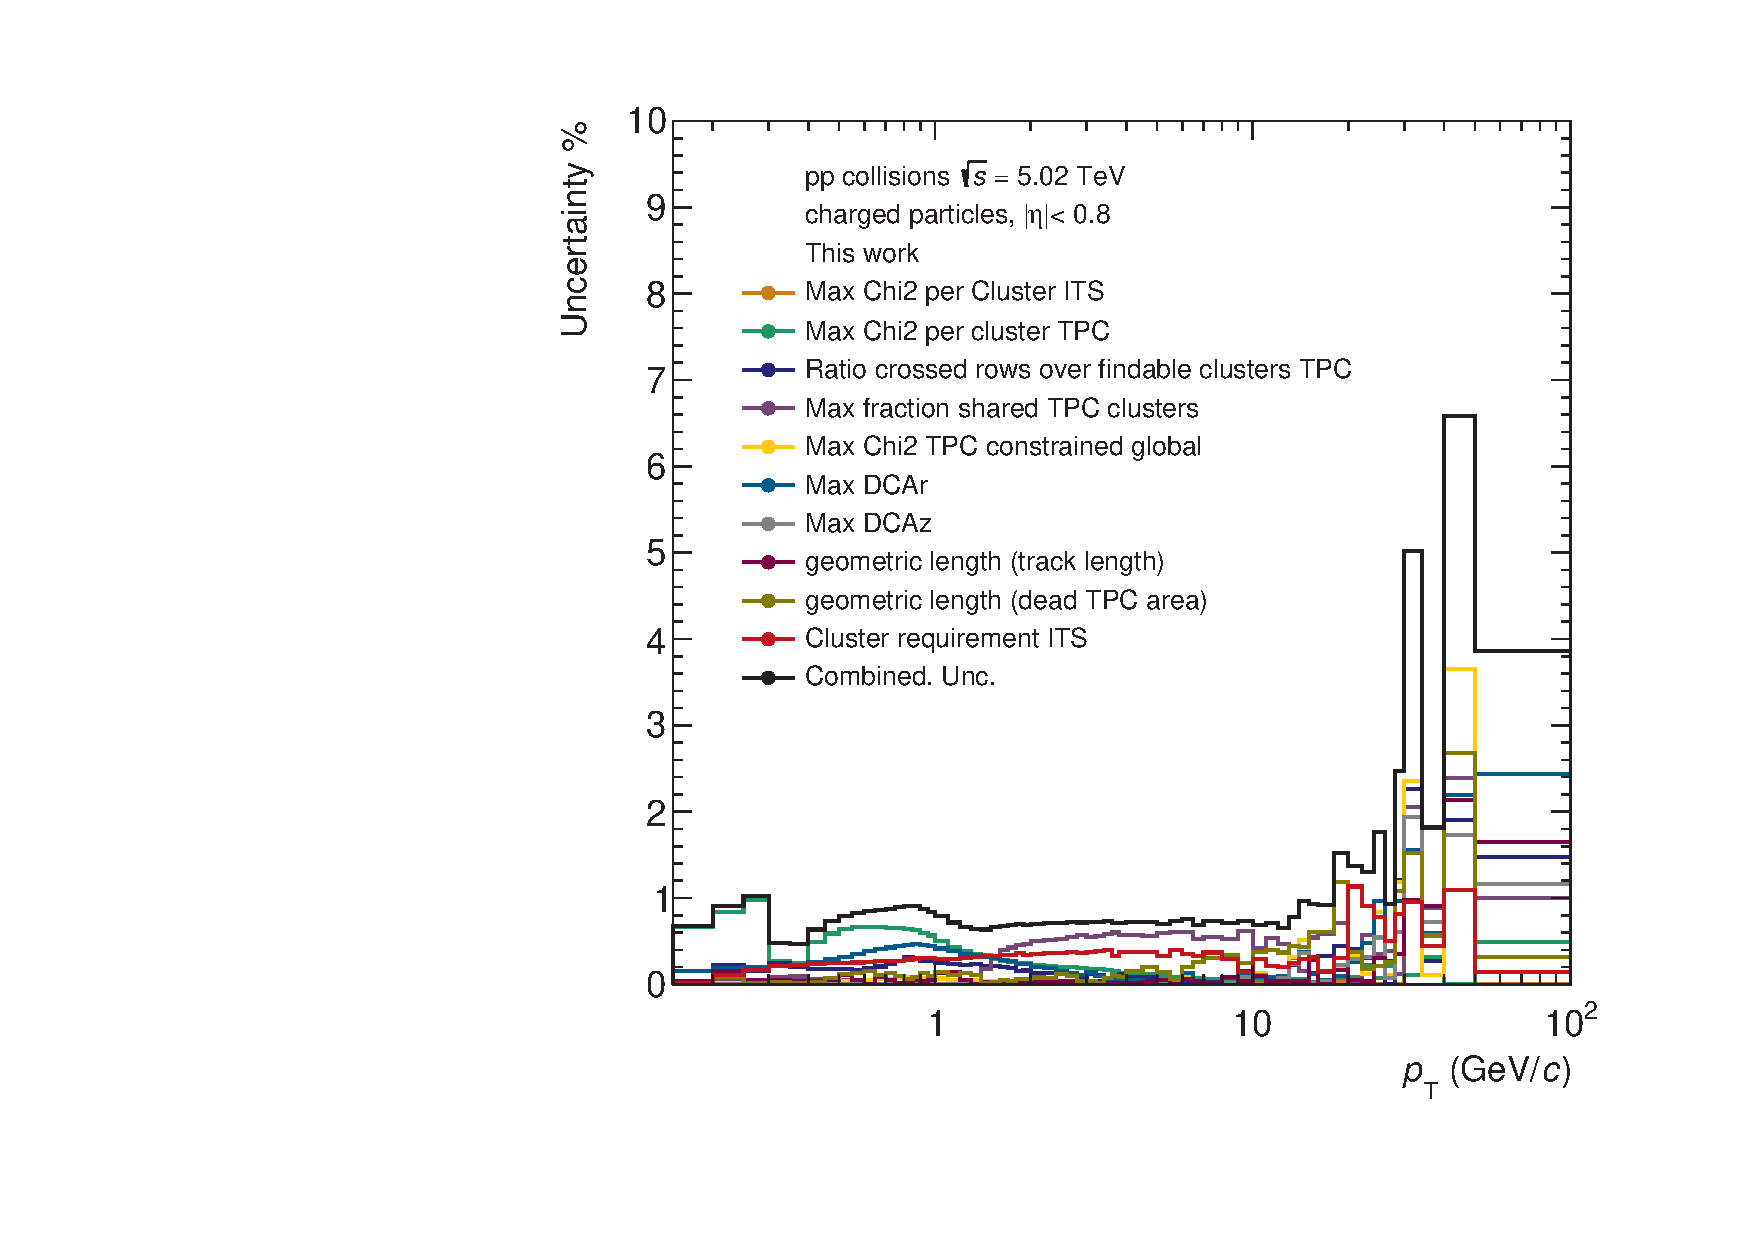
\includegraphics[width=0.495\textwidth]{Plots/SysUncpp.pdf}  
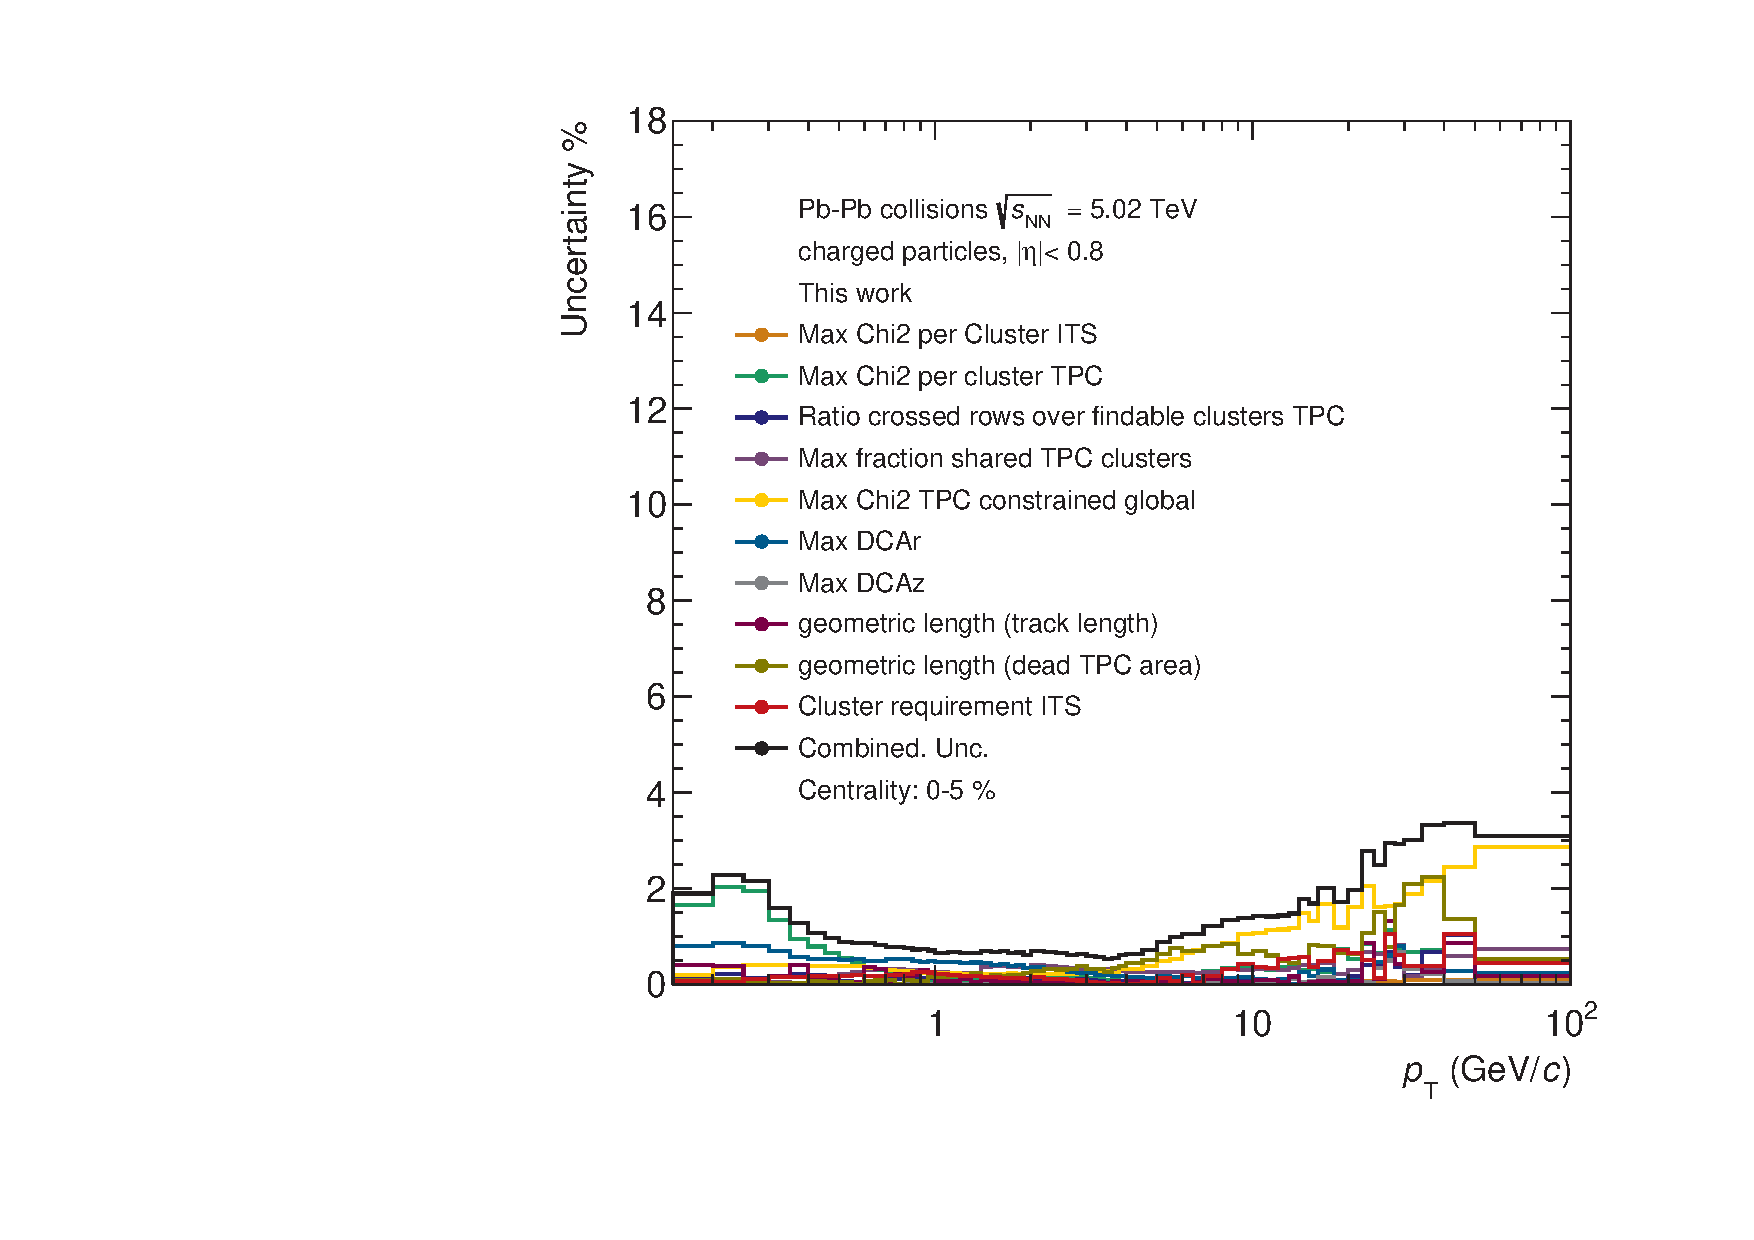
\includegraphics[width=0.495\textwidth]{Plots/SysUncPbPbcent.pdf}  
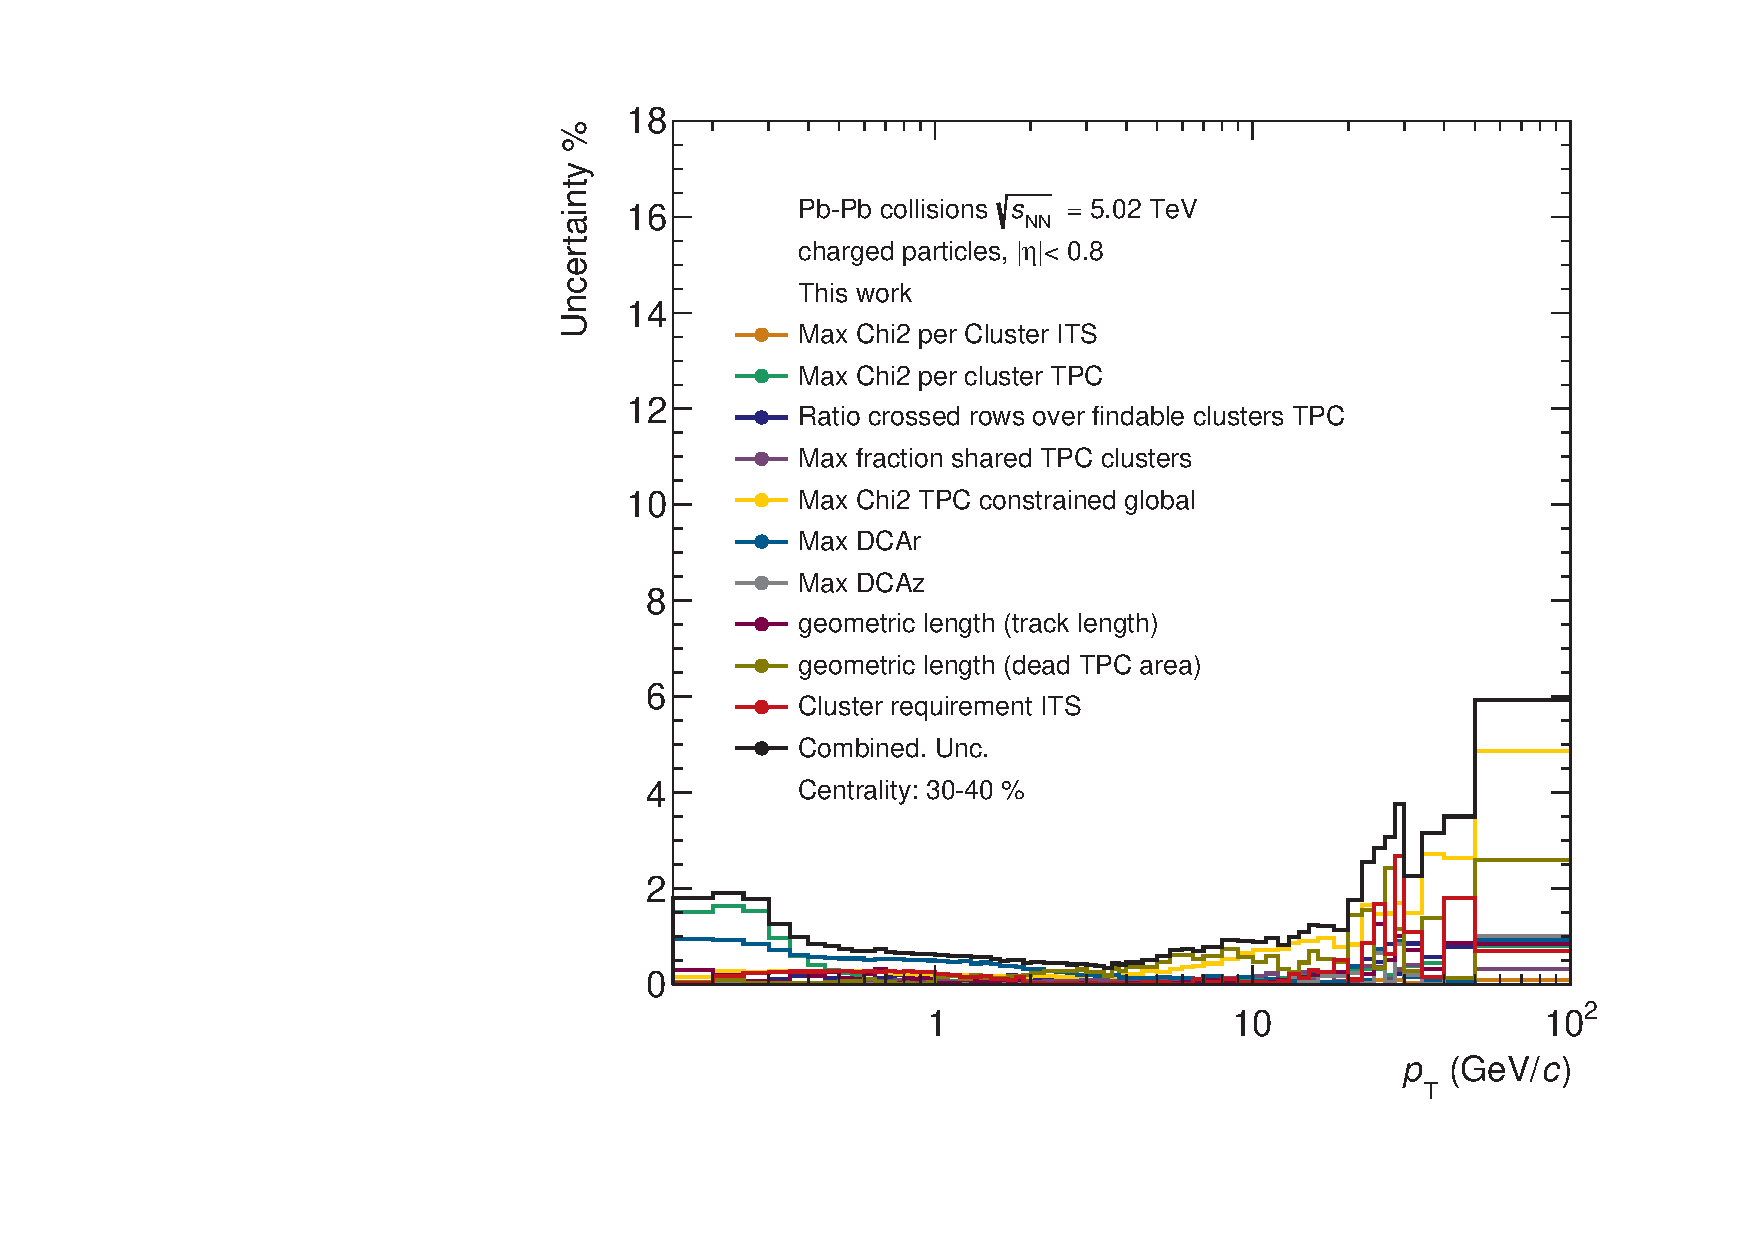
\includegraphics[width=0.495\textwidth]{Plots/SysUncPbPbsemi.pdf}  
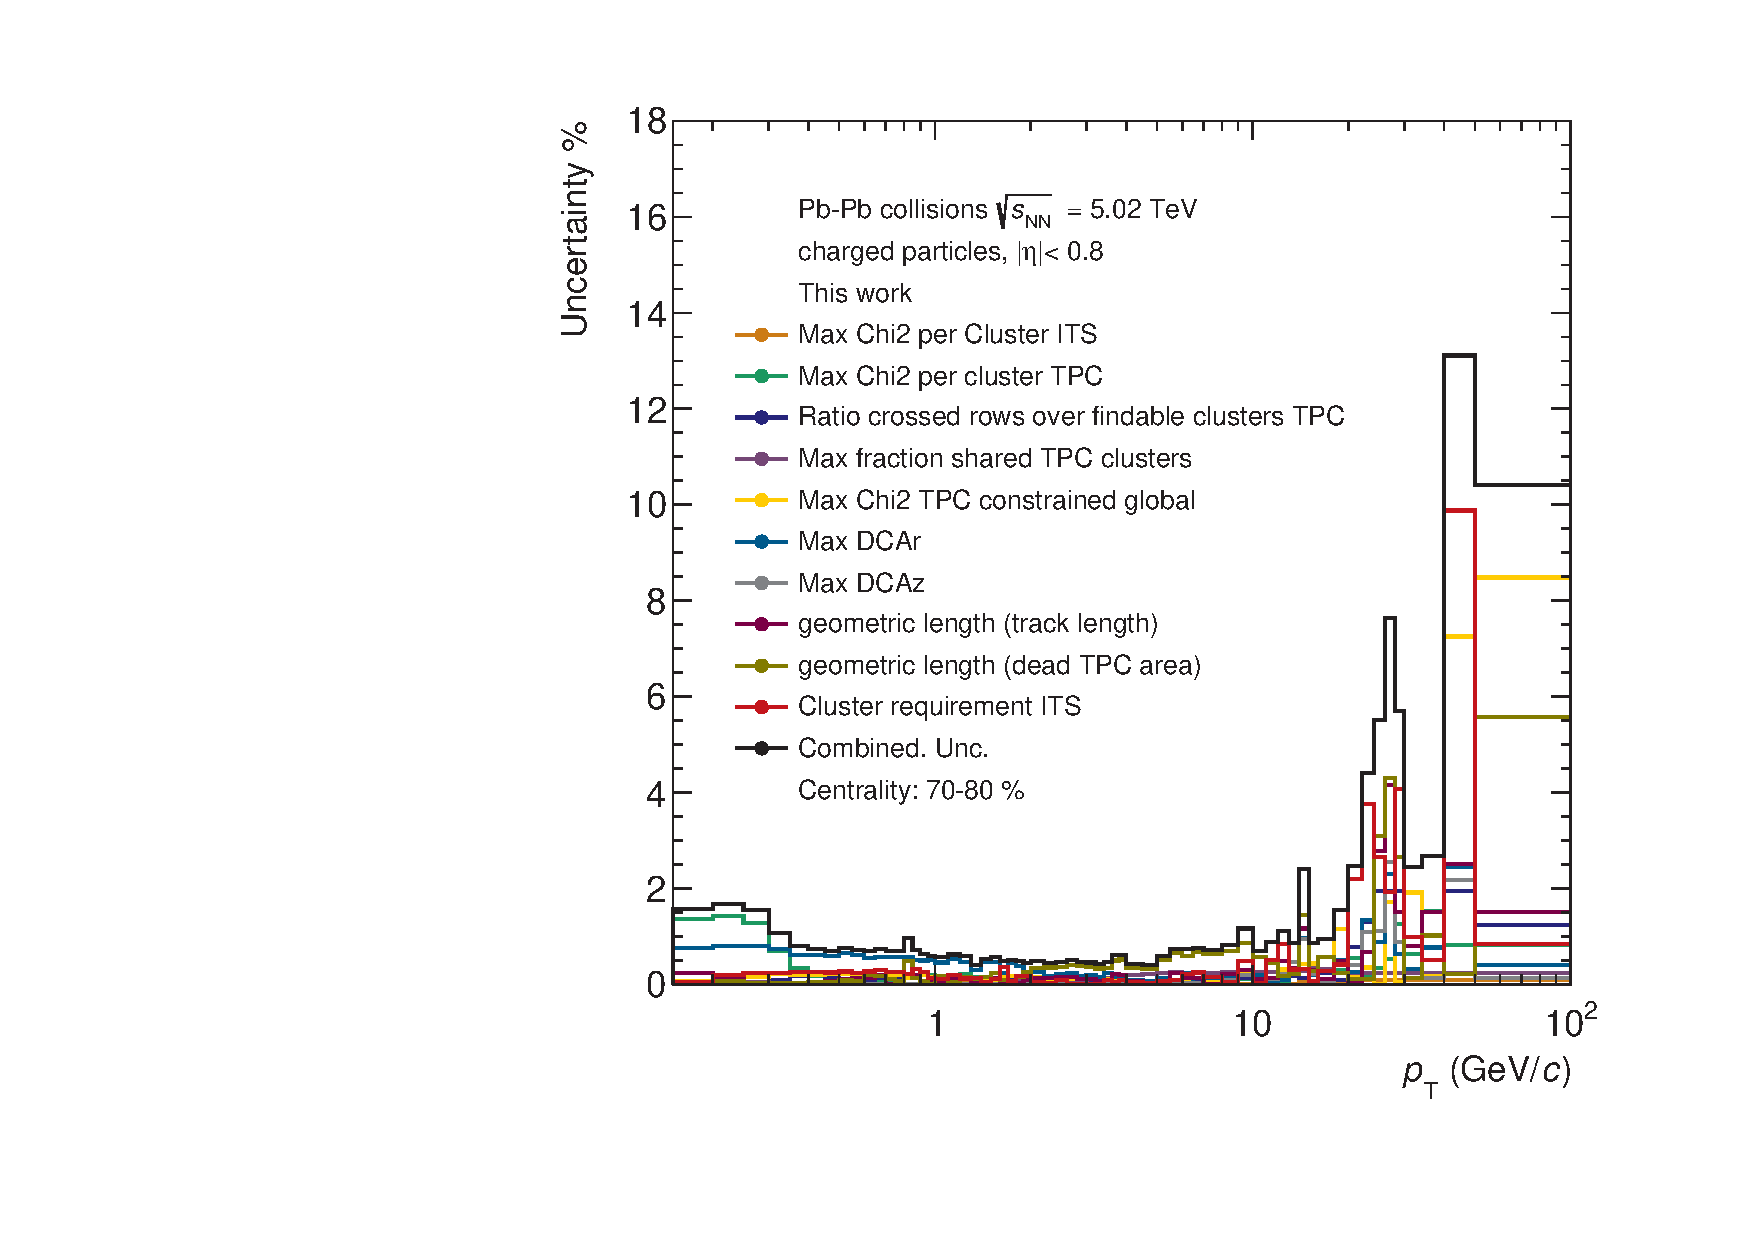
\includegraphics[width=0.495\textwidth]{Plots/SysUncPbPbperi.pdf}  
\caption{Relative systematic uncertainties of the \pt spectra from the track selection for pp as well as central, semi-central and peripheral Pb-Pb collisions.}
\label{SysUncSpec}
\end{figure}
\begin{figure}[H]
\centering
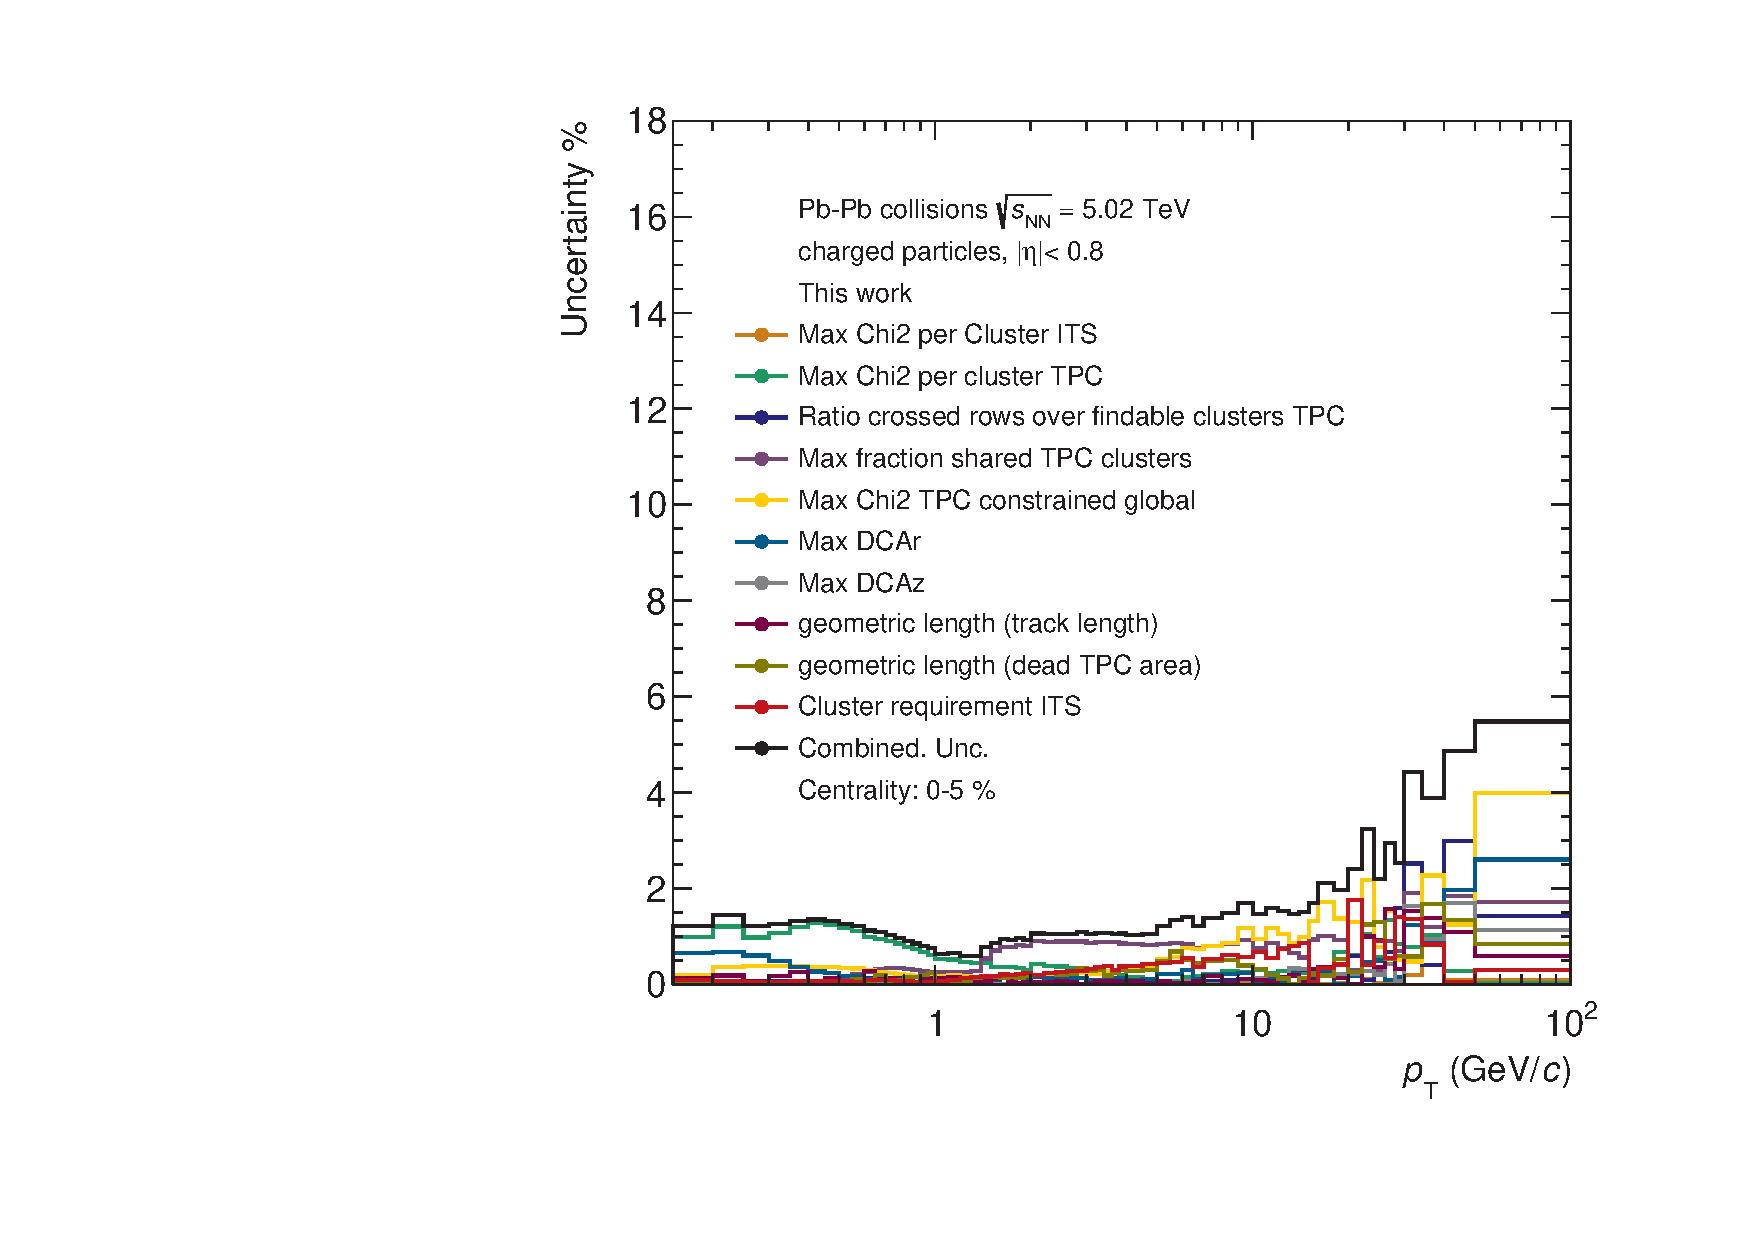
\includegraphics[width=0.495\textwidth]{Plots/SysUncRaacent.pdf}  
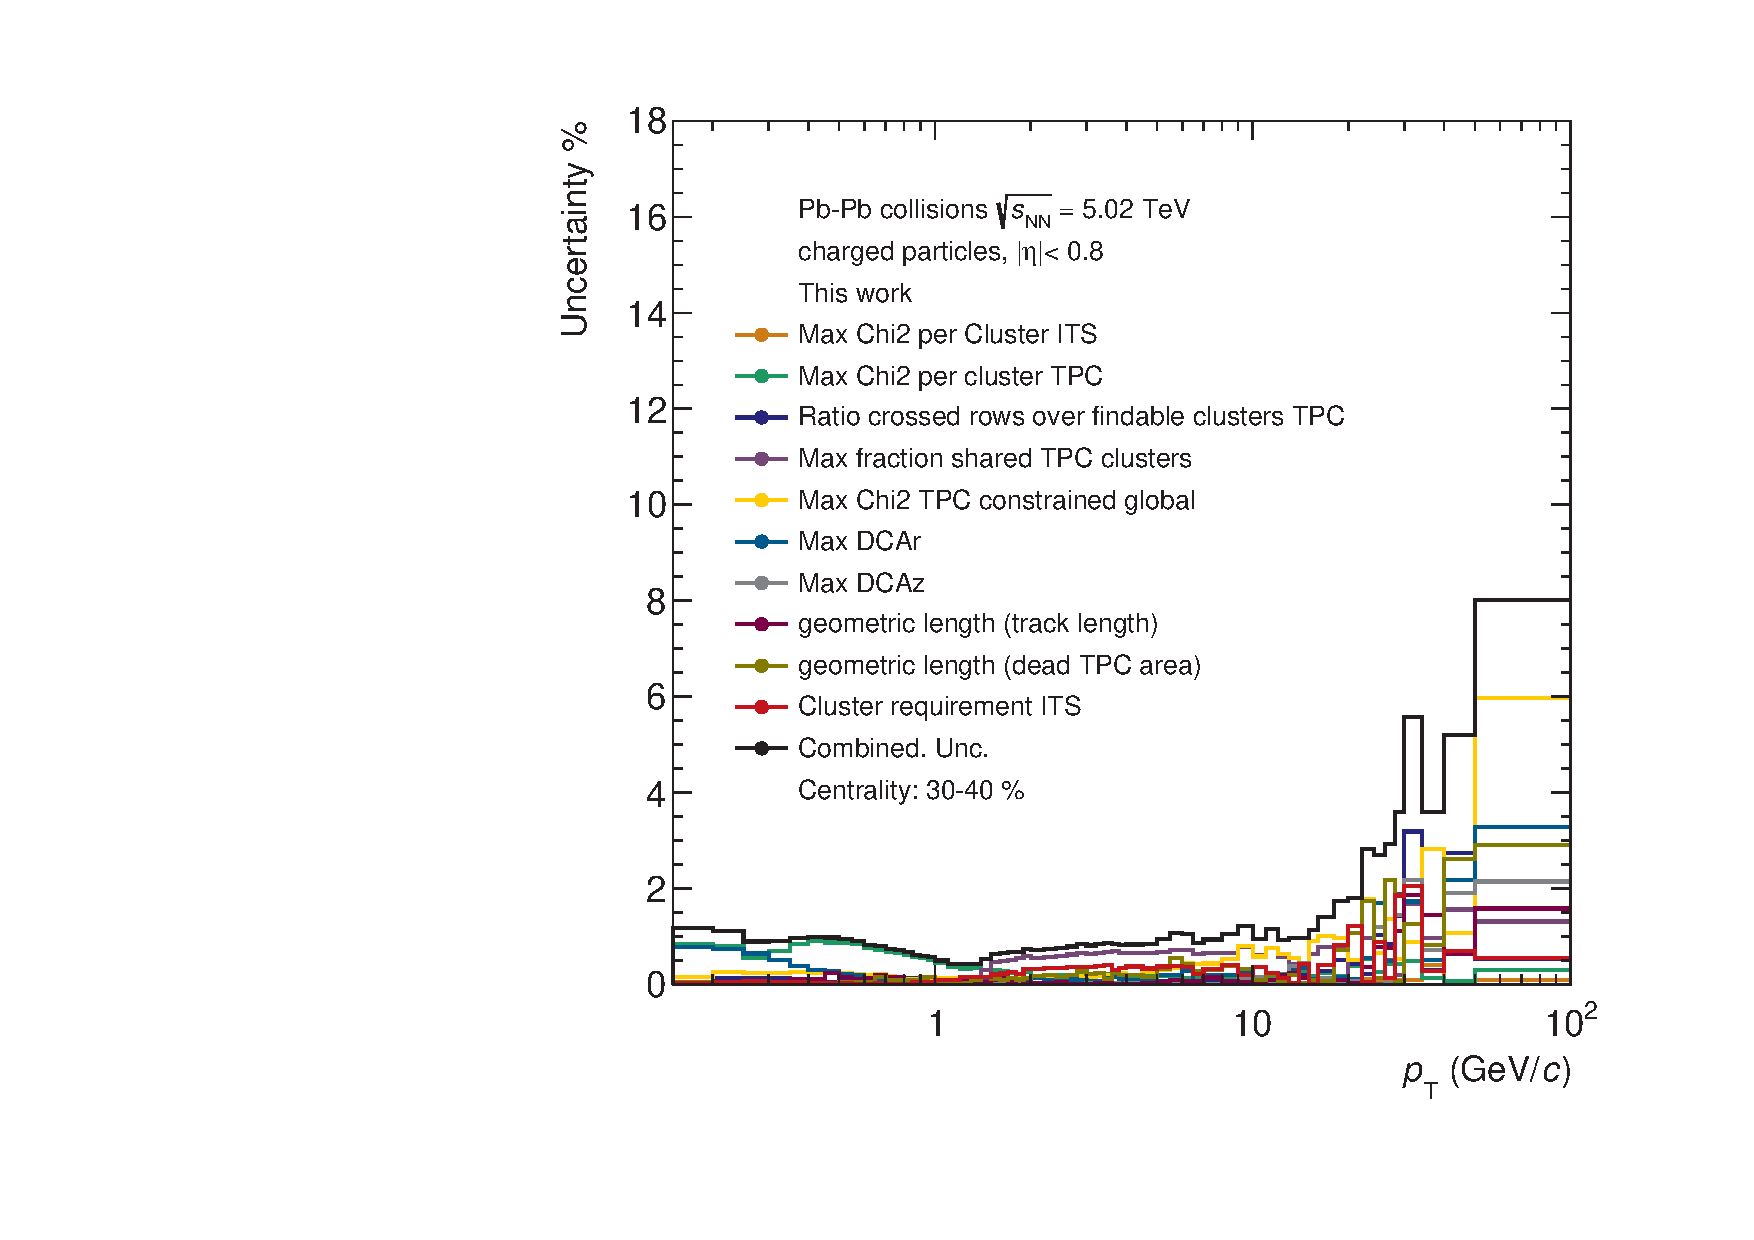
\includegraphics[width=0.495\textwidth]{Plots/SysUncRaasemi.pdf}  
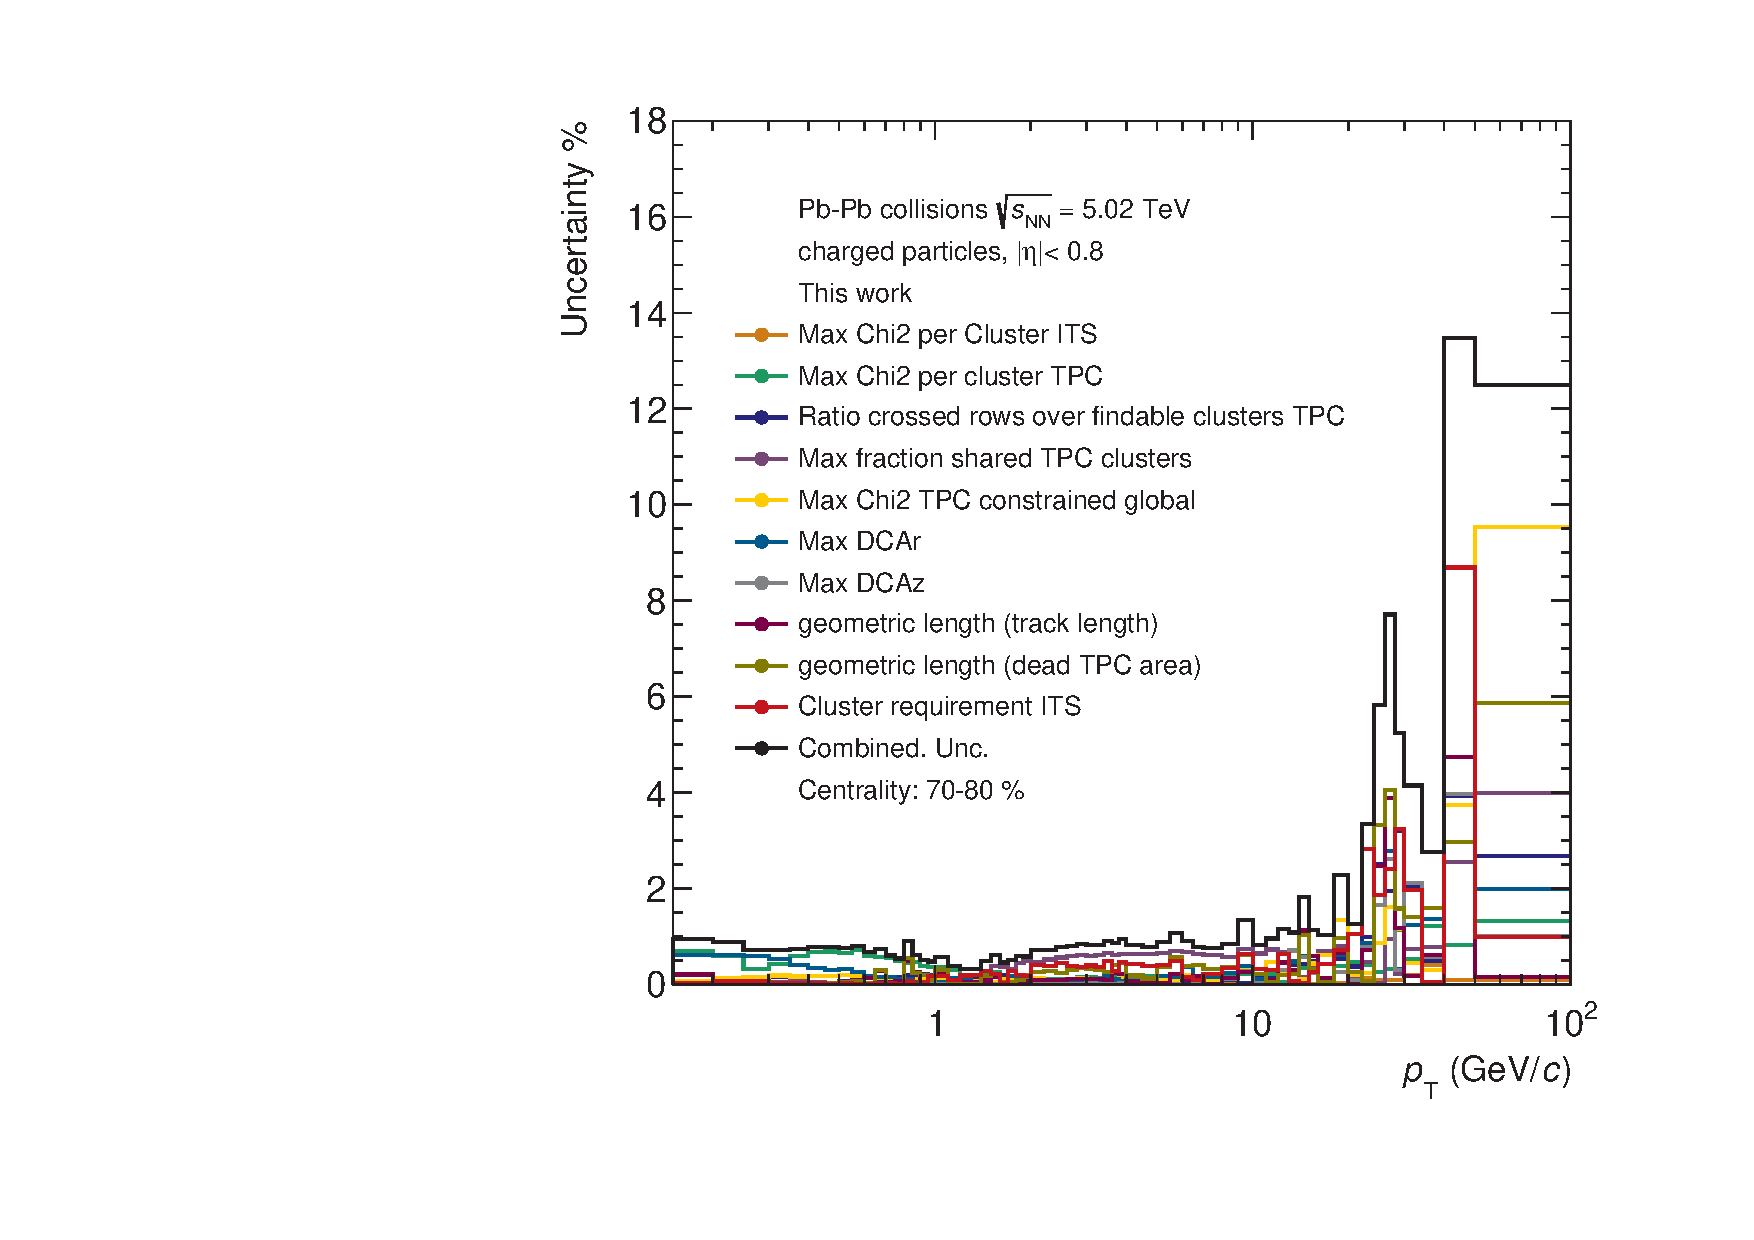
\includegraphics[width=0.495\textwidth]{Plots/SysUncRaaperi.pdf}  
\caption{Relative systematic uncertainties of $R_\text{PbPb}$ from the track selection for central, semi-central  and peripheral Pb-Pb collisions.}
\label{SysUncRaa}
\end{figure}
\subsection{Other sources} 
In previous measurements of inclusive charged particles (cite paper), other sources of systematic uncertainties on the \pt distributions besides the track selection have been identified. In this section, an overview about the corresponding sources as well as an approximation of their contributions to the total systematic uncertainties acquired from the cited publication will be given. In Table \ref{tab:othersources}, the relative systematic uncertainties for \pt spectra in pp and Pb-Pb collisions are shown. 
\begin{enumerate} 
\item The tracking efficiency is approximated using the MC information. Nevertheless, the simulations are not able  to reproduce fully the detector performance. The related systematic uncertainty is calculated by means of a quantity that compares global tracks with tracks reconstructed only with the TPC: the matching efficiency. The maximum deviation from unity of the ratio of the matching efficiency in MC to the one in data is used as uncertainty.
\begin{table}[tb!]
\renewcommand{\arraystretch}{1.5}
%\rowcolor{bodyBlue}
\centering
\begin{tabular}{l c c}
\toprule
\rowcolor{headerBlue}  \textbf{Source of uncertainty} &  \textbf{pp}  &   \textbf{Pb-Pb}  \\
\midrule
\midrule
Matching efficiency & $0.0$-$1.1\%$  & $0.2$-$1.2\%$\\
Particle composition & $0.2$-$2.4\%$ & $0.2$-$2.0\%$\\
Secondary scaling & $0.0$-$2.8\%$ & $0.0$-$4.5\%$ \\
Vertex and trigger efficiency & $0.0$-$1.2\%$ & - \\
Material budget & $0.1$-$0.9\%$ & $0.1$-$0.9\%$ \\
Anchor point & - & $0.06$-$3.5\%$ \\
\bottomrule
\end{tabular}
\caption{Contributions to the total systematic uncertainty on \pt distributions in pp and Pb-Pb collisions calculated in the previous ALICE measurements (cite paper).}
\label{tab:othersources}
\end{table}
\item There are three distinct contributions to the systematic uncertainty of the particle composition correction (cite Patrick). For their calculation, variations in specific parameters of the approach are performed and the maximal deviation between the nominal correction and the one resulting from each variation is assigned as systematic uncertainty. The total systematic uncertainty is determined by summing in quadrature the individual contributions:
\iffalse
\begin{itemize}
\item The first contribution is related to measured production rates of identified charged particles. The measured particle spectrum of each particle type are varied between the extreme values of the range of its systematic uncertainty.
\item Another contribution arises from the extrapolation of the \pt spectra at low \pt used in the correction. The contribution is determined by recalculating the correction using alternative parametrizations as well as different fit ranges.
\item The last contribution originates from the fact that the relative particle abundances are assumed to be flat for $p_\text{T} > 10$ GeV/$c$. For the calculation of the systematic uncertainty, this range is varied and the resulting corrections are compared to the nominal one.  
\end{itemize} 
\fi
\item The contribution to the systematic uncertainties of the data-driven scaling of the secondary contamination is determined by comparing the correction factors that result from a two and a three template fit. The deviation between both results is assigned as uncertainty.
\item In the published results, the vertex and trigger efficiency is combined and the half of this value was assigned as systematic uncertainty.
\item The simulation of the impact of the detector material on the data by the MC productions is subject to systematic uncertainties. Through an analysis of photon conversions, the related systematic uncertainty is found varying the material budged in the simulation by $\pm 4.5\%$.
\item For the centrality determination in Pb-Pb collisions, an anchor point is defined as the reference limit of the centrality below which the measurement is biased. This is used  the scale of the centrality. Its determination is subject to an uncertainty of $0.5\%$. After adjusting the centrality boundaries with this uncertainty, \pt spectra are recalculated and the maximum deviation from the nominal one is assigned as the corresponding contribution.
\end{enumerate} 

\section{Results}
\subsection{Differential cross section in pp collisions}
After implementing the corrections as described in Section \ref{secCorr}, the differential cross section (see Equation \ref{EqdiffCross}) for inclusive charged particles in inelastic pp collisions at $\sqrt{s}=5.02$ TeV measured by ALICE is presented in Figure \ref{diffCross}. The statistical uncertainties are shown in error bars, while the boxes represent the systematic uncertainties determined in Section \ref{systracksel}. In the figure, the previous ALICE measurement (cite note) is also shown. It can be observed that the presented work reaches a transverse momentum of $p_\text{T} = 100$ GeV/$c$ which extends the \pt reach of the previous measurement of $p_\text{T} = 50$ GeV/$c$. This development is explained by the higher statistics that the used data sets offer in comparison to the ones of 2015. Another feature of this result is the improved granularity of the \pt intervals which are finer in the mid and high \pt region than in the previous results. These two aspects facilitate a better precision of the nuclear modification factors as it will be seen in the following sections. 
\begin{figure}[tb!]
\centering
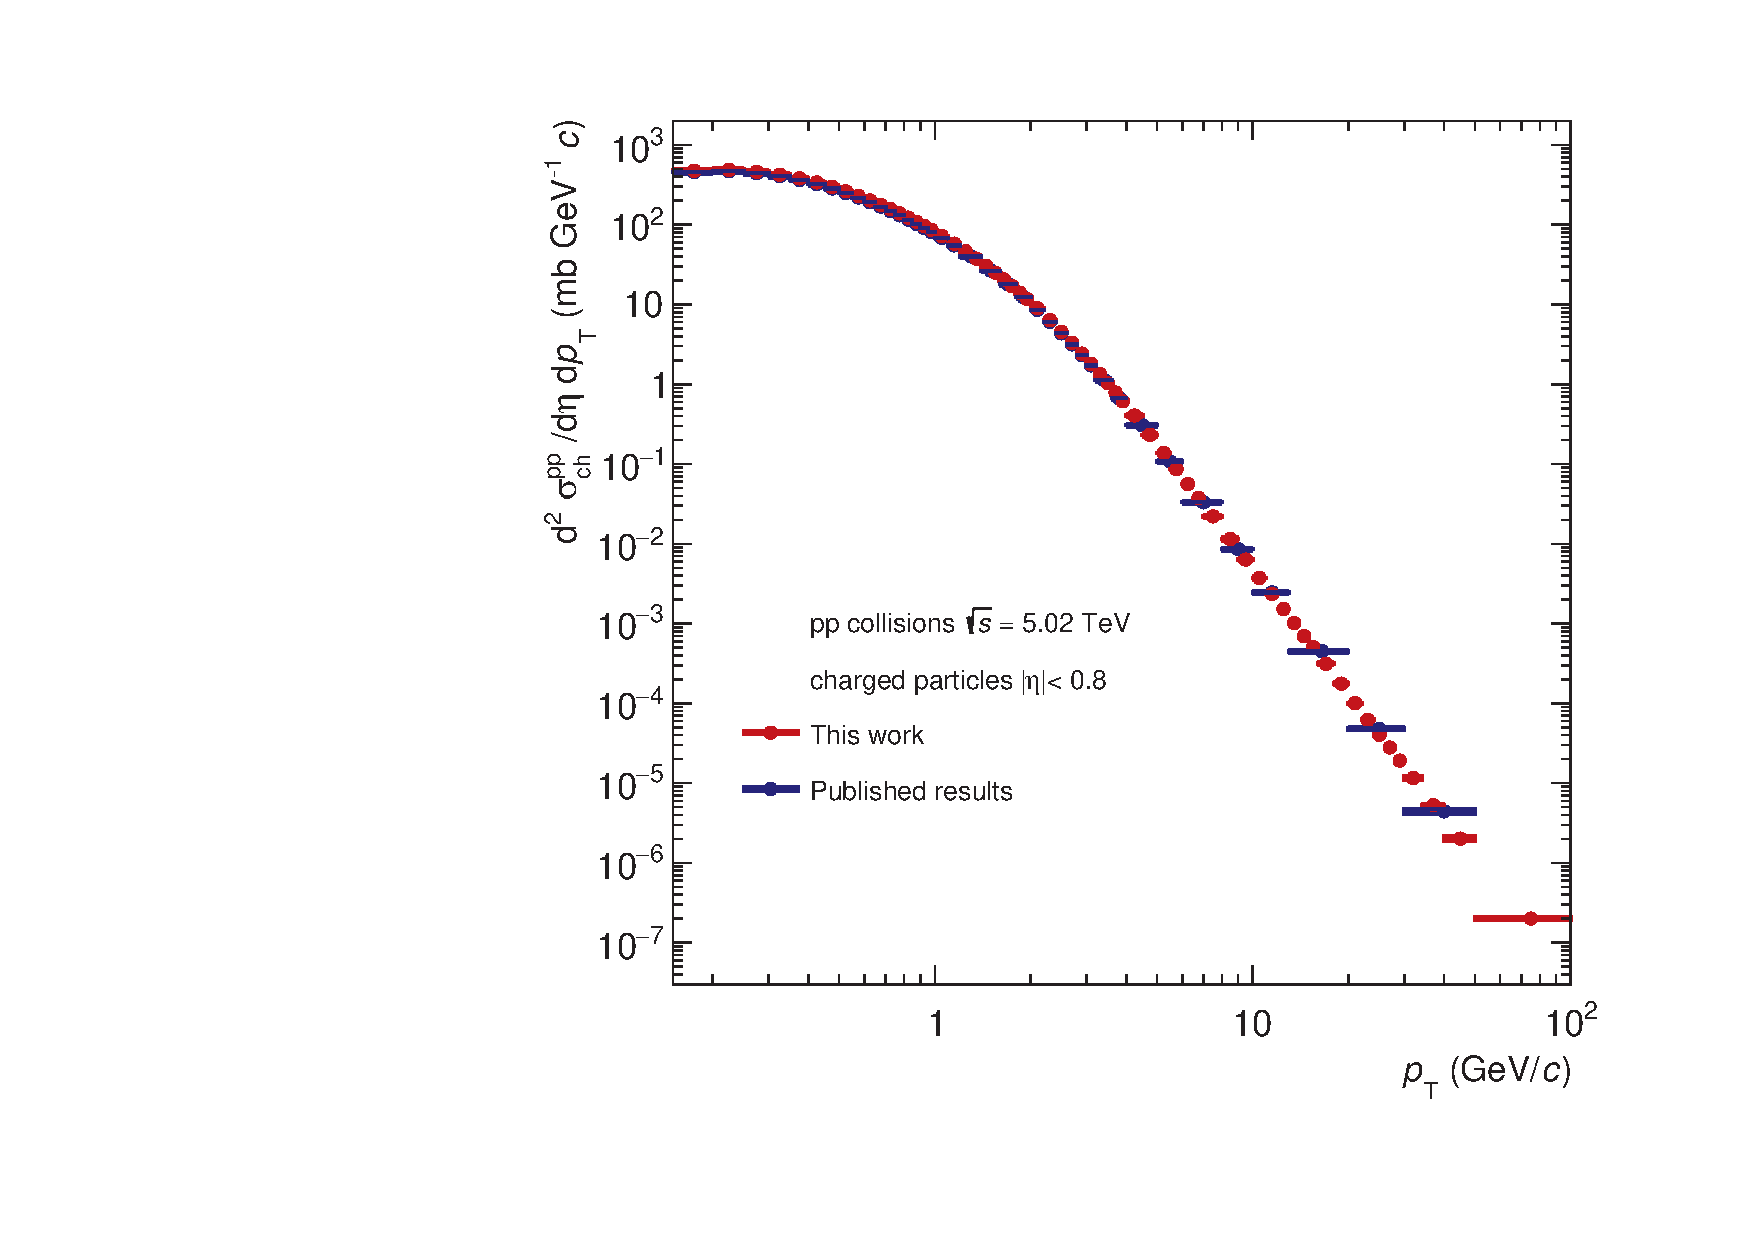
\includegraphics[width=12cm]{Plots/diffCrosspp.pdf}  
\caption{Differential cross section for inclusive charged-particle production in pp collisions at $\sqrt{s}=5.02$ TeV measured by ALICE.}
\label{diffCross}
\end{figure}
\subsection{Invariant yield in Pb-Pb collisions}
The invariant yields (see Equation \ref{Eqinyield}) for inclusive charged particles in nine centrality classes in inelastic Pb-Pb collisions measured by ALICE at $\sqrt{s}_\text{NN}=5.02$ TeV are given in Figure \ref{invYield}. Statistical and systematic uncertainties are represented with error bars and boxes, respectively. In the same figure, the results of the previous ALICE measurement are also shown. The shape of the \pt distributions present a dependency on the centrality. In central collisions, the invariant yields present a more pronounced slope for \pt > 3 GeV/$c$ than the one in peripheral collisions. With decreasing centrality the shape becomes more similar to the one in pp. Once determined the fully \pt distributions in pp and in Pb-Pb collisions, the calculation of nuclear modification factors is performed.
\begin{figure}[tb!]
\centering
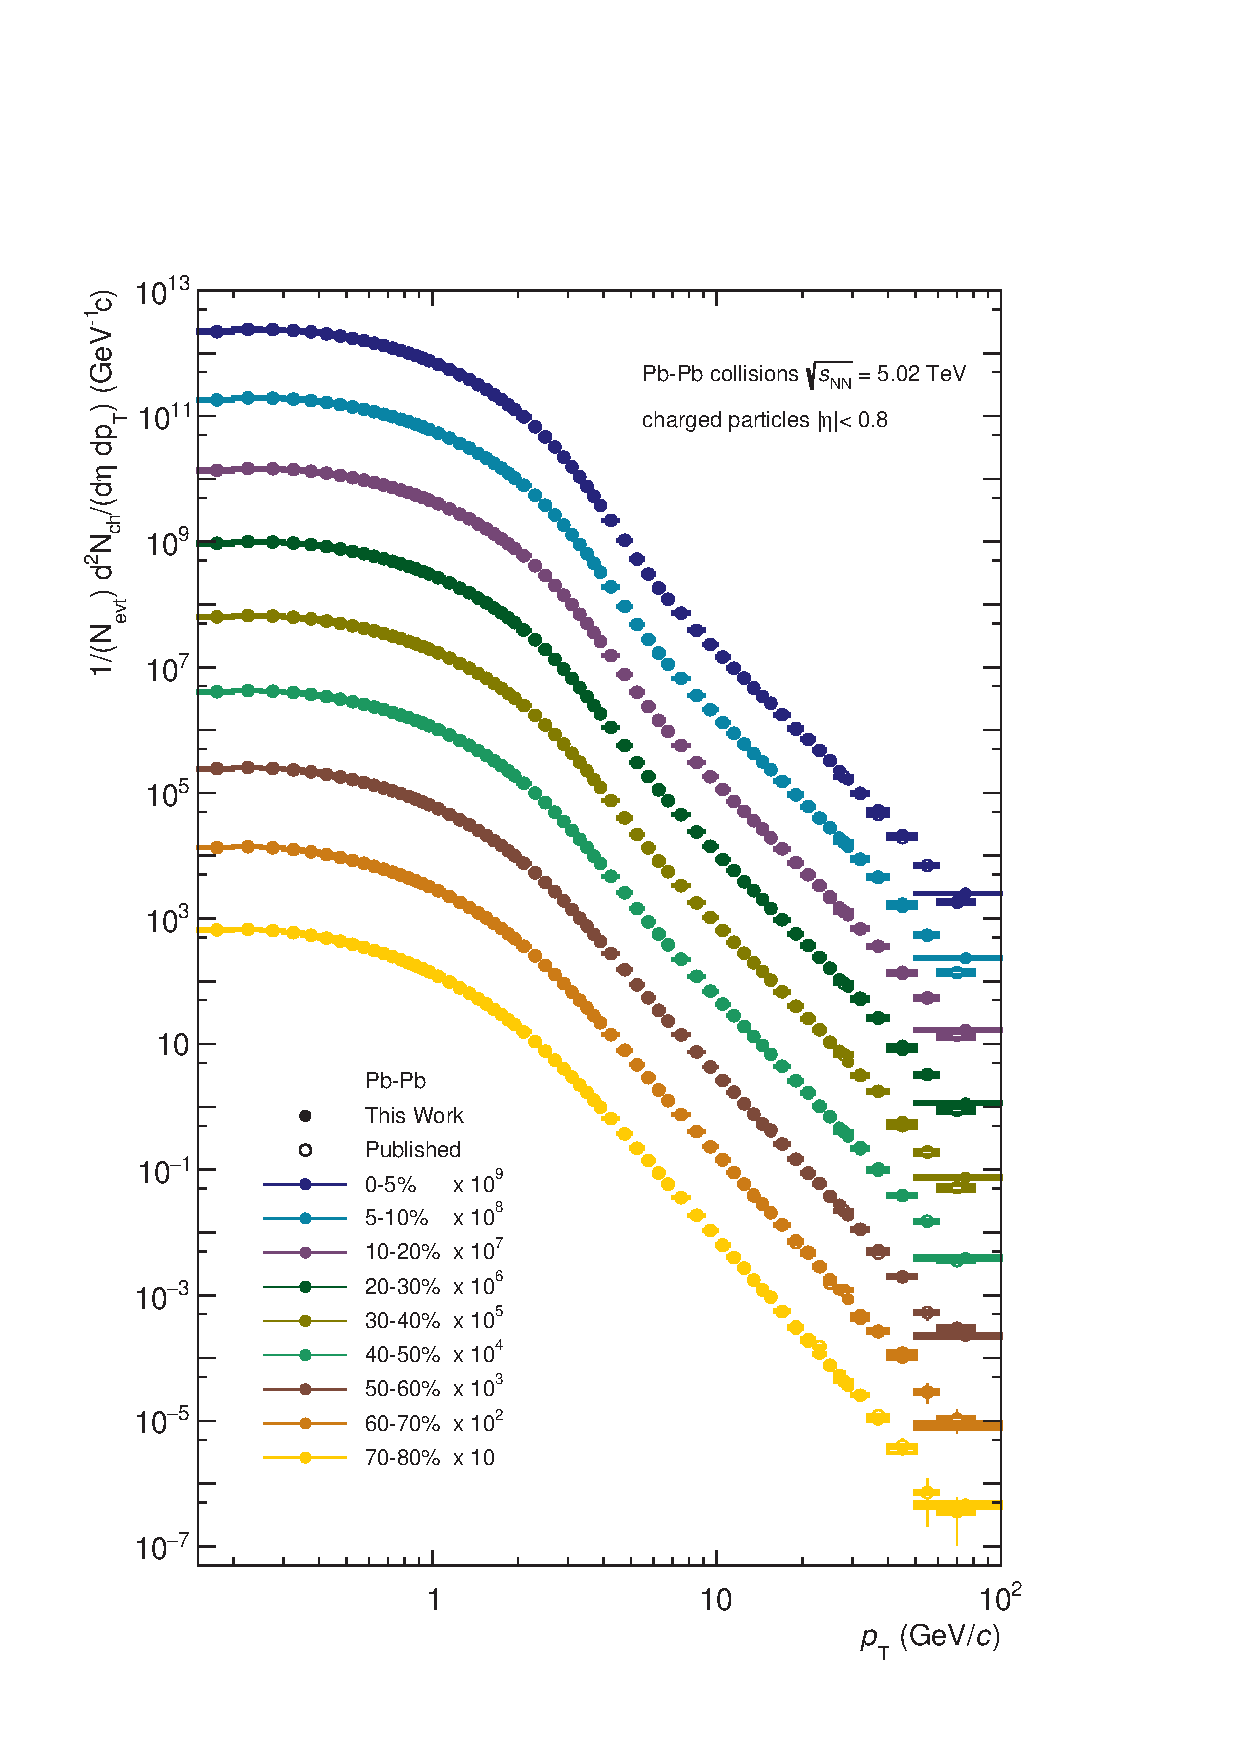
\includegraphics[width=12cm]{Plots/invYieldPbPb.pdf}  
\caption{Differential cross section for inclusive charged-particle production in pp collisions at $\sqrt{s}=5.02$ TeV measured by ALICE.}
\label{invYield}
\end{figure}
\subsection{Nuclear modification factors}
As introduced in Section (cite section), the energy density produced in ultra-relativistic heavy-ion collisions  allows the creation of a quark-gluon plasma, a deconfined state of strongly interacting matter. In this medium, high \pt partons experience an energy loss which leads to a suppression of the particle production as it was suggested by J.D. Bjorken. The study of this suppression can therefore provide insight on the properties of the quark-gluon plasma. In the presented work, the suppression is analyzed through a comparison of the charged-particle production in heavy-ion collisions with a reference measurement in pp collisions, where no quark-gluon plasma is expected to be created. The nuclear modification factor $R_\text{PbPb} $ offers the possibility to quantify the suppression via:
\begin{equation}
R_\text{PbPb} = \dfrac{1}{\langle T_\text{AA}\rangle} \dfrac{\text{d}^2 N^\text{Pb-Pb}_\text{ch} / \text{d}\eta \text{d}p_\text{T}}{\text{d}^2 \sigma^\text{pp}_\text{ch} / \text{d}\eta \text{d}p_\text{T}}
\end{equation}
where the numerator represents the invariant yield in Pb-Pb collisions and the denominator the differential cross section in pp collisions. Note that the differential cross section is scaled with the nuclear overlap function $\langle T_\text{PbPb} \rangle$. This quantity is calculated through a Glauber Monte Carlo simulation (cite ana note) and the values used in this work can be found in Table \ref{tab:taa}.\\
\begin{table}[tb!]
\renewcommand{\arraystretch}{1.5}
%\rowcolor{bodyBlue}
\centering
\begin{tabular}{l c c}
\toprule
\rowcolor{headerBlue}  \textbf{Centrality} &  \textbf{$\mathbf{\langle T_\text{PbPb} \rangle}$ ($\text{mb}^{-1}$)}  &   \textbf{sys. Unc. } ($\text{mb}^{-1}$) \\
\midrule
\midrule
0-5\% & $26.08$  & $0.176$\\
5-10\% & $20.44$ & $0.166$\\
10-20\% & $14.4$ & $0.126$ \\
20-30\% & $8.767$ & $0.101$ \\
30-40\% & $5.086$ & $0.0814$ \\
40-50\% & $2.747$ & $0.0486$\\
50-60\% & $1.352$ & $0.0309$\\
60-70\% & $0.5992$ & $0.0158$\\
70-80\% & $0.2385$ & $0.00552$ \\
\bottomrule
\end{tabular}
\caption{Nuclear overlap function with the corresponding systematic uncertainties for Pb-Pb collisions at $\sqrt{s}_\text{NN}=5.02$ TeV in the studied centrality classes obtained with a Glauber Monte Carlo simulation (cite ana note).}
\label{tab:taa}
\end{table}
In Figure \ref{Raa}, the nuclear modification factors for inclusive charged particles in inelastic Pb-Pb collisions measured by ALICE at $\sqrt{s}_\text{NN}=5.02$ TeV are presented in nine centrality classes. Here, the statistical uncertainties are denoted as error bars and the systematic uncertainties as boxes. As expected, the nuclear modification factors are characterized by a strong dependency on the centrality. In the same figure, the previous measurements of nuclear modification factors in ALICE are also shown with open markers. The results of this work are in good agreement with the ones of the previous measurement. There is an improvement of the \pt reach as well as of the granularity of the intervals for \pt > 3.2 GeV/$c$. This is result of the increased statistics in pp collisions which allows a better precision in the corresponding \pt distribution as described before.\\
A significant suppression of the charged-particle production is observed in most \pt intervals of the nine centrality classes. In the low \pt region, the suppression decreases slightly until the $R_\text{PbPb}$ reach values of around 0.45 in the most central collisions and around 0.8 in peripheral collisions. Following this peak, the maximal suppression occurs at around \pt = 6.5 GeV/$c$ for the first four centrality classes, before the nuclear modification factors rise gradually and reach values between around 0.5 and 0.6. Towards peripheral collisions, the fall after the peak is less pronounced, the factors grow more steeply and the values of $R_\text{PbPb}$ approach unity at high transverse momenta. 
\begin{figure}[tb!]
\centering
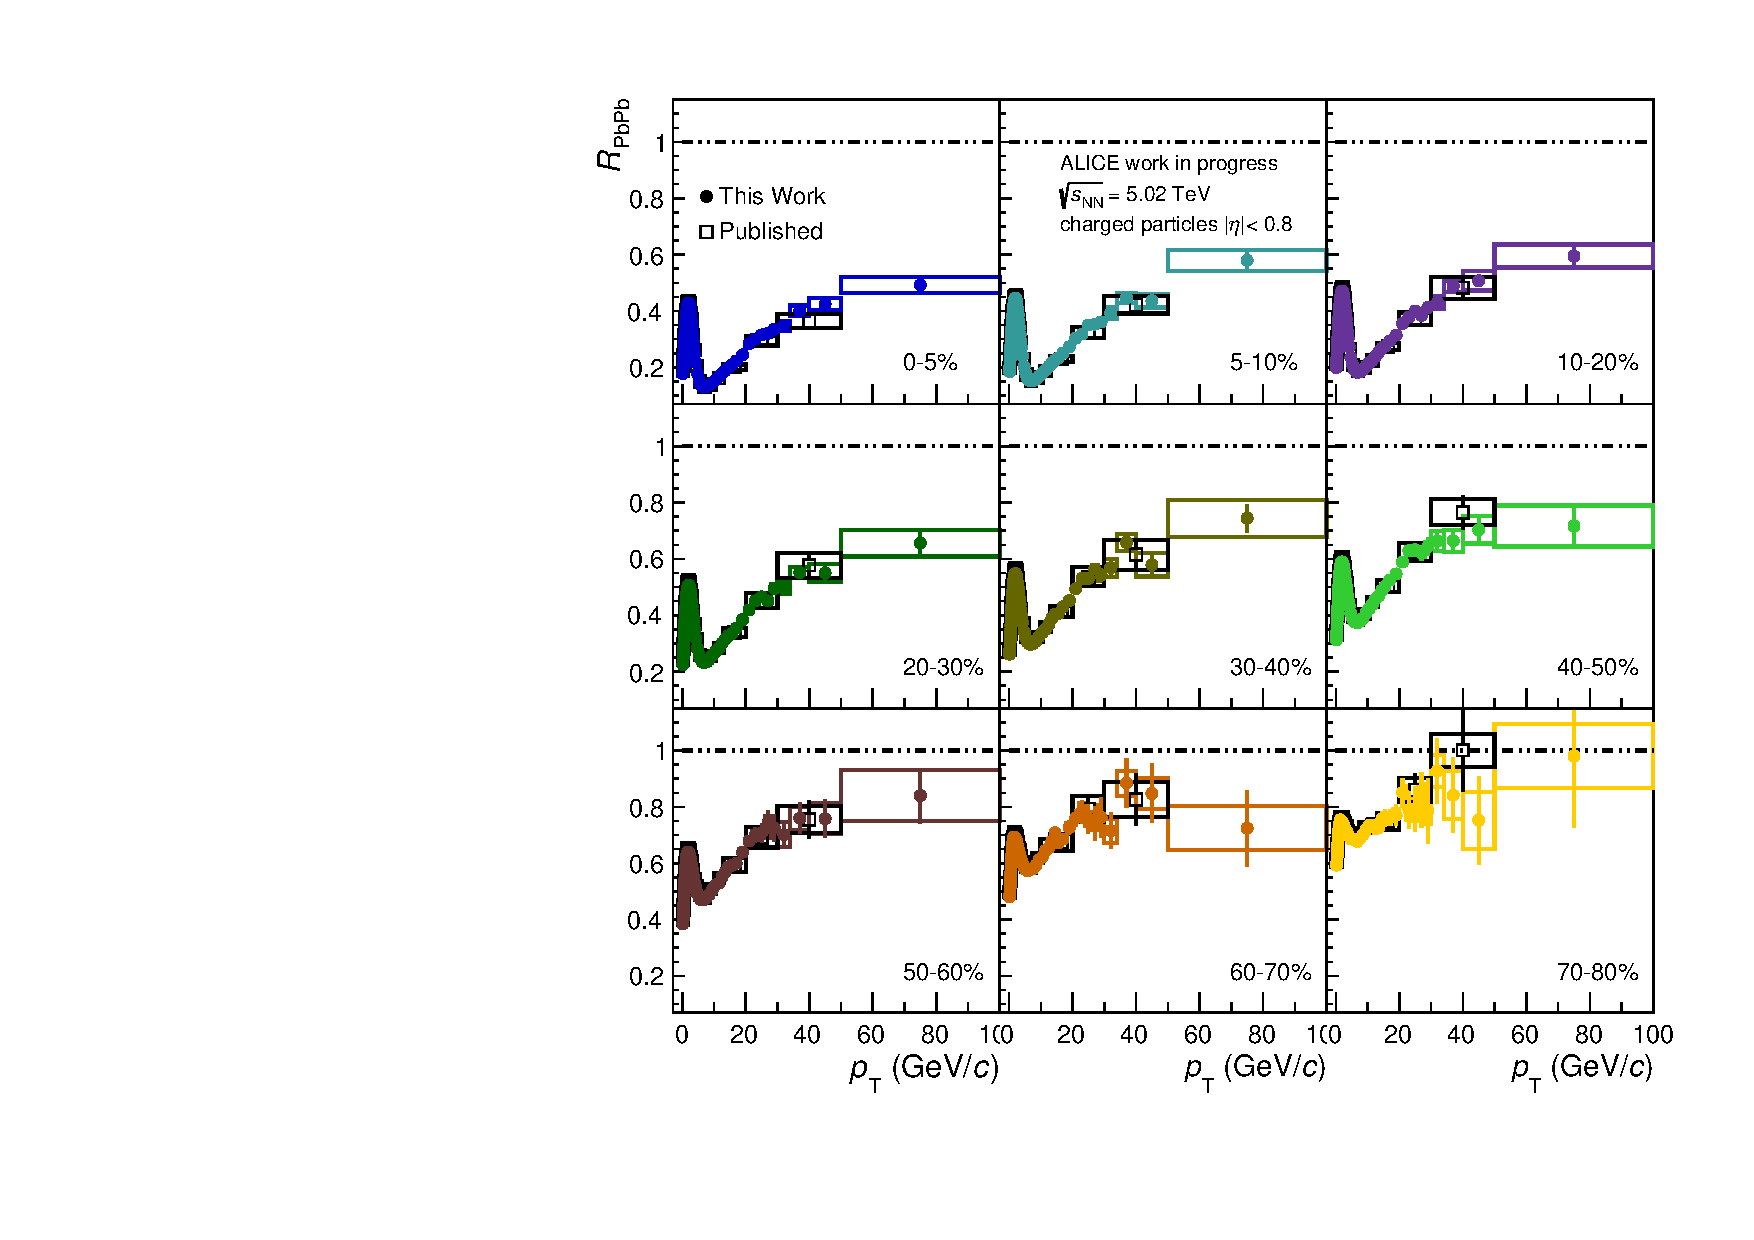
\includegraphics[width=12cm]{Plots/Raa.pdf}  
\caption{Nuclear modification factors for nine centrality classes in Pb-Pb collisions at $\sqrt{s}=5.02$ TeV measured by ALICE.}
\label{Raa}
\end{figure}
For a better understanding of the suppression in heavy-ion collisions, several theoretical models make predictions about the behavior of physical observables in the strong interacting medium at LHC energies. It is worth comparing the obtained results with the theoretical models in order to proof their validity in more detail. To this end, the nuclear modification factor for the most central collisions obtained in this work is compared to four different theoretical formalisms. The calculations of these models make use of the pQCD factorization of the cross section for hadron production. All of the following models implement different approaches which lead to parton energy loss. Therefore, a comparison of these measurements with the models will help to improve the fundamental understanding of parton energy loss mechanisms. The formalisms of each of the approaches are presented briefly in the following (cite paper):
\begin{figure}[tb!]
\centering
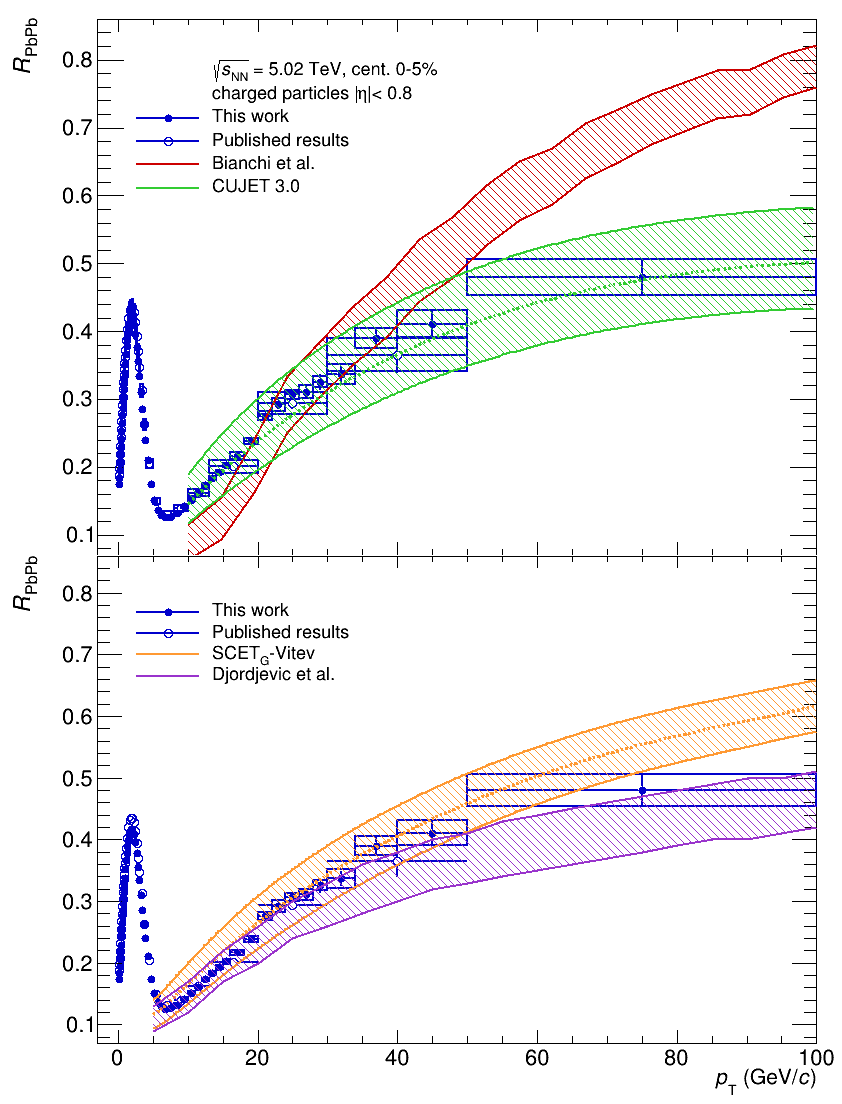
\includegraphics[width=10	cm]{Plots/Raatheo.png}  
\caption{Nuclear modification factors for the most central collisions in Pb-Pb collisions at $\sqrt{s}=5.02$ TeV compared to four theoretical prediction as well as to the previous ALICE publication.}
\label{raatheo}
\end{figure}

\begin{enumerate}
\item \textbf{Bianchi:} This model (cite here) describes the production of high \pt hadrons with the fragmentation of hard partons. Employing an approach based on the hydrodynamics, the energy loss of the parton is characterized by the medium transport coefficient $\hat q$ scaled with the temperature dependent entropy density and the energy scale of jets within the medium.
\item \textbf{CUJET 3.0:} Here (cite here), the pQCD formalism provided by its predecessor CUJET 2.0 is upgraded with a description of soft processes by means of a suppression of quark and gluon degrees of freedom and the emergence of chromomagnetic monopoles. In the framework, the model prediction is calculated by varying the QCD running coupling and the ratio of electric to magnetic screening scales.
\item $\mathbf{SCET}_\mathbf{G}$-\textbf{Vitev:} This description (cite here) of inclusive particle production and the suppression consists in the soft-collinear effective theory (SCET) extended with the coupling of Glauber gluons exchanges to the medium. In the calculations, cold nuclear matter effects and parton-to-hadron fragmentation functions are taken into account.
\item \textbf{Djordjevic:} The last approach predicts the energy loss with pQCD calculations in a dynamical QCD medium of finite spatial extent. In the framework of the $\text{SCET}_\text{G}$ model, the prediction discusses the radiative and the collisional energy loss of the partons integrating cold nuclear effects.
\end{enumerate}
In Figure \ref{raatheo}, the measured nuclear modification factor for a centrality of 0-5\% is compared to the four theoretical models as well as to the previous ALICE measurement. The upper and lower boundaries of the models represent the uncertainty which is calculated through variation of different parameters of the corresponding approaches. The measured nuclear modification factors are overall consistent with the theoretical models. Nevertheless, the Bianchi model overestimates the suppression in the \pt range 10 < \pt < 18 GeV/$c$, which can only be stated using this work due to its higher statistics in pp collisions.

\begin{appendices}
\chapter{Appendix}
\section{Tracking efficiency}
\label{TrkEffApp}
\end{appendices}

%, by virtue of its technical characteristics
%underlying
%drawbacks
%coined
%establishes
%is resolved
%streamlined
%resemble
%yields
%pronounced
%stand-alone
%exploting
%exhibit
%these outliers
%exemplify
%arises (from the fact)
%build upon
%notions
%conceive
%gathered data
%data collections
%procedure
%overall
%accounts for
% The way in which this is done
%  It is worth pointingout


%Quellen: https://home.cern/science/physics/standard-model
%An Introduction to Particle Physics and the Standard Model by Robert Mann
%An Introduction to Particle Physics and the Standard Model of Particle Physics by Cottingham and Greenwood
%Physics Of The Standard Model And Beyond, The Chong-sa Lim, Toshiyuki Morii,
%Data sample: https://twiki.cern.ch/twiki/bin/view/ALICE/AliDPGReconstructedDataTakingPeriodsSummarypp5

\end{document}
